\documentclass[11pt,a4paper,draft,oneside,openany]{memoir}

\usepackage[english]{babel}
\usepackage[utf8]{inputenc}
\usepackage[T1]{fontenc}
\usepackage[british]{isodate}

% Layout Fixes
\usepackage{booktabs} % nicer spacing between table rulers
\usepackage{microtype}
\usepackage{fixltx2e} % To prevent the figures from being placed
                      % out-of-order with respect to their
                      % "non-starred" counterparts


\usepackage{amsmath,amssymb, amsbsy}
\usepackage[amsmath,amsthm,thmmarks]{ntheorem}
\usepackage[final]{graphicx}
\usepackage[export]{adjustbox}
\usepackage{float}
\usepackage{pdfpages}
\usepackage{color}
\usepackage{fancyvrb}
\usepackage{semantic}
\usepackage{etoolbox}
\usepackage{environ}
\usepackage{newtxtext}
\usepackage{newtxmath}

\usepackage[final]{listings}
% Fix dashes in listings (from
% https://tex.stackexchange.com/questions/33185/listings-package-changes-hyphens-to-minus-signs
% )
\makeatletter
\lst@CCPutMacro\lst@ProcessOther {"2D}{\lst@ttfamily{-{}}{-{}}}
\@empty\z@\@empty
\makeatother

% Avoid breaking lstlistings environments across pages.
\BeforeBeginEnvironment{lstlisting}{\vspace{\topskip}\par\noindent\begin{minipage}{\linewidth}}
\AfterEndEnvironment{lstlisting}{\end{minipage}\par}
\newenvironment{wrap}{\vspace{\topskip}\par\noindent\begin{minipage}{\linewidth}}{\end{minipage}\par}

\renewcommand{\ttdefault}{pcr} % Courier instead of Computer Modern

\usepackage{enumitem} % Allows \begin{description}[style=nextline]

\usepackage{fixme}
\fxsetup{
    author=,
    layout=margin,
    theme=color
}

\makeatletter
\newcommand*\idstyle{%
        \expandafter\id@style\the\lst@token\relax
}
\def\id@style#1#2\relax{%
        \ifcat#1\relax\else
                \ifnum`#1=\uccode`#1%
                        \color{blue}
                \fi
        \fi
}
\makeatother

% Bibliography
%\usepackage[style=alphabetic,natbib=true]{biblatex}
\usepackage[
hyperref=auto,
backend=biber,
style=alphabetic,
citestyle=alphabetic,
defernumbers=true
]{biblatex}

\usepackage[hyperindex,hidelinks]{hyperref}
\usepackage[capitalise,noabbrev]{cleveref}

% Fonts
\usepackage{fontspec}
\usepackage{palatino}
\linespread{1.05}
\setmonofont[Scale=MatchLowercase]{DejaVu Sans Mono}

% customize chapter pages
\makepagestyle{myheadings}
\makepagestyle{myheadingschapterpage}
\makeevenfoot{myheadingschapterpage}{}{\thepage}{}
\makeoddfoot{myheadingschapterpage}{}{\thepage}{}
\aliaspagestyle{chapter}{myheadingschapterpage}
\aliaspagestyle{title}{myheadingschapterpage}
\makeevenhead{myheadings}{\hskip.5cm\leftmark}{}{}
\makeoddhead{myheadings}{}{}{\rightmark\hskip.5cm}
\makeevenfoot{myheadings}{}{\thepage}{}
\makeoddfoot{myheadings}{}{\thepage}{}
\pagestyle{myheadings}

\def\thefigure{\arabic{figure}}
\setcounter{tocdepth}{0}


\setsecnumdepth{subsection}
\setcounter{chapter}{0}
\setsecheadstyle{\large\bfseries\raggedright}
\setsubsecheadstyle{\bfseries}

% BIBLIOGRAPHY styling
% Print the DOI url out

\DeclareFieldFormat{doi}{\textsc{doi}: \url{http://dx.doi.org/#1}}
\DeclareNameAlias{default}{last-first/first-last}
%\DeclareFieldFormat{title}{\emph{#1}}
\renewcommand\mkbibnamefirst[1]{\textsc{#1}}
\renewcommand\mkbibnamelast[1]{\textsc{#1}}
\renewcommand*{\bibfont}{\footnotesize}

% No page numbers for parts in TOC
\cftpagenumbersoff{part}

% Figures

\usepackage{sidecap}
\usepackage{caption}
\captionsetup{margin=0pt, font=small, labelfont=bf, format=hang}
% \setlength{\abovecaptionskip}{0pt}
% \setlength{\belowcaptionskip}{0pt}
\captionsetup[subfigure]{skip=1em}
\usepackage{subcaption}

% Default commands
\newcommand{\subimgwidth}{.48\textwidth}
\newcommand{\imgwidth}{.85\textwidth}


\newtheorem{example}{Example}
%
\theoremstyle{plain}
\theoremsymbol{\tiny $\Box$}
\newtheorem{definition}[equation]{Definition}


% Bitwise and and or operators
% http://tex.stackexchange.com/questions/39313/double-nested-logical-and-and-logical-or-symbols
\DeclareFontFamily{U}{matha}{\hyphenchar\font45}
\DeclareFontShape{U}{matha}{m}{n}{
      <5> <6> <7> <8> <9> <10> gen * matha
      <10.95> matha10 <12> <14.4> <17.28> <20.74> <24.88> matha12
      }{}

\newcommand{\bland}{\mathbin{
  \raisebox{.1ex}{%
    \rotatebox[origin=c]{-90}{\usefont{U}{matha}{m}{n}\symbol{\string"CE}}}}}
\newcommand{\blor}{\mathbin{
  \raisebox{.1ex}{%
    \rotatebox[origin=c]{90}{\usefont{U}{matha}{m}{n}\symbol{\string"CE}}}}}

% Visually Separate figures from text using a line.
\def\topfigrule{\vskip1ex\noindent\dotfill}
\def\botfigrule{\noindent\dotfill\vskip1ex}

% Useful macros.
\newcommand{\tagsc}[1]{\tag{\textsc{#1}}} % Fake Small Caps tagging
\newcommand*{\bfrac}[2]{\genfrac{}{}{0pt}{}{#1}{#2}}


%%% Local Variables: 
%%% mode: latex
%%% TeX-master: "thesis.tex"
%%% End: 

% Define Language
\lstdefinelanguage{futhark}
{
  % list of keywords
  morekeywords={
    do,
    else,
    for,
    fun,
    if,
    in,
    include,
    let,
    loop,
    struct,
    then,
    type,
    val,
    while,
    with,
    module,
    where,
  },
  sensitive=true, % keywords are not case-sensitive
  morecomment=[l]{--}, % l is for line comment
  morecomment=[s]{\{-}{-\}}, % s is for start and end delimiter
%  otherkeywords={>,<,=,<=,>=,!,*,/,-,+,|,&,||,&&,==,=>},
  morestring=[b]" % defines that strings are enclosed in double quotes
}

% Define Colors
\usepackage{xcolor}
\definecolor{eclipseBlue}{RGB}{42,0.0,255}
\definecolor{eclipseGreen}{RGB}{63,127,95}
\definecolor{eclipsePurple}{RGB}{127,0,85}

\newcommand{\fop}[1]{\mbox{\ttfamily\color{eclipseBlue}#1}}
\newcommand{\fw}[1]{\mbox{\ttfamily\bfseries\color{eclipsePurple}#1}}

% Set Language
\lstset{
  language={futhark},
  basicstyle=\ttfamily, % Global Code Style
  captionpos=b, % Position of the Caption (t for top, b for bottom)
  extendedchars=true, % Allows 256 instead of 128 ASCII characters
  tabsize=2, % number of spaces indented when discovering a tab
  columns=fixed, % make all characters equal width
  keepspaces=true, % does not ignore spaces to fit width, convert tabs to spaces
  showstringspaces=false, % lets spaces in strings appear as real spaces
  breaklines=true, % wrap lines if they don't fit
  frame=trbl, % draw a frame at the top, right, left and bottom of the listing
  frameround=tttt, % make the frame round at all four corners
  framesep=4pt, % quarter circle size of the round corners
  numbers=left, % show line numbers at the left
  numberstyle=\small\ttfamily, % style of the line numbers
  commentstyle=\slshape\bfseries\color{eclipseGreen}, % style of comments
  keywordstyle=\bfseries, % style of keywords
  stringstyle=\color{eclipseBlue}, % style of strings
  emph=[1] {
    false,
    filter,
    iota,
    map,
    partition,
    rearrange,
    reduce,
    reduce_comm,
    replicate,
    reshape,
    rotate,
    shape,
    scan,
    split,
    true,
    unzip,
    write,
    zip,
    stream_seq,
    stream_red,
    stream_map,
    size,
  },
  emphstyle=\ttfamily\bfseries,
  moredelim=**[is][\color{red}]{@}{@}
}

\newcommand{\kt}[1]{\textsf{#1}}
\newcommand{\kw}[1]{\mbox{\texttt{\bfseries{#1}}}}
\newcommand{\id}[1]{\mbox{\it{#1}}}
\def\M{\kw{M}}
\newcommand{\Mv}[2]{\M~\overline{#1}~\overline{#2}}
\newcommand{\Loop}{\kw{loop}}
\newcommand{\Do}{\kw{do}}
\newcommand{\For}{\kw{for}}
\newcommand{\Map}{\kw{map}}
\newcommand{\Reduce}{\kw{reduce}}
\newcommand{\Scan}{\kw{scan}}
\newcommand{\Transpose}{\kw{transpose}}
\newcommand{\Let}[3]{\kw{let}~#1~\mbox{\texttt{=~}}#2~\kw{in}~#3}
\newcommand{\If}[3]{\kw{if}~#1~\kw{then}~#2~\kw{else}~#3}
\newcommand{\vd}{\vdash}
\newcommand{\Rearrange}{\kw{rearrange}}
\newcommand{\Replicate}{\kw{replicate}}
\newcommand{\Par}[1]{\mathtt{(}#1\mathtt{)}}
\newcommand{\StreamMap}{\kw{stream\_map}}
\newcommand{\StreamRed}{\kw{stream\_red}}
\newcommand{\StreamSeq}{\kw{stream\_seq}}
\newcommand{\ov}[1]{\overline{#1}}
\newcommand{\nseq}[2]{\overline{#1}^{(#2)}}

%%% Local Variables:
%%% mode: latex
%%% TeX-master: "thesis"
%%% End:


\lstset{
  language=Futhark,
  basicstyle=\ttfamily\small,
  keywordstyle=\bfseries,
  showlines=true,
  columns=fullflexible,
  keepspaces=true,
  numbers=left,
  stepnumber=1,
}

\usepackage[titelside, en, nat]{ku-forside}

\titel{My Thesis}
\undertitel{And its Subtitle}
\forfatter{Troels Henriksen -- \texttt{athas@sigkill.dk}}
\forfatterET{}
\forfatterTO{}
\opgave{PhD thesis} % Findes kun under 'titelside'
\dato{2017}
\vejleder{Supervisors: Cosmin Eugen Oancea and Fritz Henglein}

% Write "Part II" etc. in TOC instead of just "II"
\renewcommand*{\cftpartname}{Part\space}

\bibliography{thesis}

\begin{document}
\frontmatter

 \clearpage

\maketitle
~
\vspace{3cm}
  \begin{abstract}
\begin{abstract}

In this thesis we describe the design and implementation of Futhark, a
small data-parallel purely functional array language that offers a
machine-neutral programming model, and an optimising compiler that
generates efficient OpenCL code for GPUs.  The overall philosophy is
based on seeking a middle ground between functional and imperative
approaches.  The specific contributions are as follows:

First, we present a moderate flattening transformation aimed at
enhancing the degree of parallelism, which is capable of exploiting
easily accessible parallelism.  Excess parallelism is efficiently
sequentialised, while keeping access patterns intact, which then
permits further locality-of-reference optimisations.  We demonstrate
this capability by showing instances of automatic loop tiling, as well
as optimising memory access patterns.

Second, to support the flattening transformation, we present a
lightweight system of size-dependent types that enables the compiler
to reason symbolically about the size of arrays in the program, and
that reuses general-purpose compiler optimisations to infer
relationships between sizes.

Third, we furnish Futhark with novel parallel combinators capable of
expressing efficient sequentialisation of excess parallelism, as well
as their fusion rules.

Fourth, in order to express efficient programmer-written sequential
code inside parallel constructs, we introduce support for safe
in-place updates, with type system support to ensure referential
transparency and equational reasoning.

Fifth, we perform an evaluation on 21 benchmarks that demonstrates the
impact of the language and compiler features, and shows
application-level performance that is in many cases competitive with
hand-written GPU code.

Sixth, we make the Futhark compiler freely available with full source
code and extensive documentation, to serve both as a basis for further
research into functional array programming, and as a useful tool
for parallel programming in practise.

\end{abstract}

\newpage

\renewcommand{\abstractname}{Resum\'e}

\begin{abstract}

  Denne afhandling beskriver designet og implementeringen af Futhark,
  et enkelt data-parallelt, sideeffekt-fri, og funktionsorienteret
  geledsprog, der frembyder en maskinneutral programmeringsmodel.  Vi
  beskriver ligeledes en optimerende Futhark-oversætter der producerer
  effektiv OpenCL-kode målrettet afvikling på GPUer.  Den overordnede
  designfilosofi er at søge en balance mellem functionsorienterede og
  imperative fremgangsmåder.  Vores konkrete bidrag er som følger:

  For det første præsenterer vi en moderat fladningstransformering,
  der er i stand til at udnytte blot den nødvendige grad af
  parallelisme, og omdanne den overskydende parallelisme til effektiv
  sekventiel kode.  Denne sekventielle kode bibeholder den oprindelige
  lageradgangsmønsterinformation, hvilket tillader yderligere
  lagertilgangsforbedringer.  Vi demonstrerer denne styrke ved at give
  eksempler på automatisk blokafvikling af løkker, samt forbedring af
  lageradgangsmønstre.

  For det andet beskriver vi, med henblik på understøttelse af
  fladningstransformeringen, et enkelt typesystem med
  størrelses-afhængige typer, der tillader oversætteren at ræsonnere
  symbolsk om størrelsen på geledder i programmet under oversættelse.
  Vores fremgangsmåde tillader genbrug af det almene repertoire af
  oversætteroptimeringer i spørgsmål om ligheder mellem størrelser.

  For det tredje udstyrer vi Futhark med en række nyskabedne
  parallelle kombinatorer der tillader effektiv sekventialisering af
  unødig parallelisme, samt disses fusionsregler.

  For det fjerde indfører vi, med henblik på at understøtte effektiv
  sekventiel kode indlejret i de parallelle sprogkonstruktioner,
  understøttelse for direkte ændringer i geledværdier, med et
  typesystem der sikrer at effekten ikke kan observeres, og at
  lighedsbaseret ræsonnering stadigvæk er muligt.

  For det femte foretager vi en ydelsessammenlining indeholdende 21
  programmer, med henblik på at demonstrere sprogets design og
  oversætteroptimeringernes indvirkning, som viser at Futhark's
  overordnede ydelse i mange tilfælde er konkurrencedygtig med
  håndskreven GPU-kode.

  For det sjette gør vi Futhark-oversætteren frit tilgængelig,
  indeholdende al kildetekst og omfattende dokumentation, således at
  den kan tjene både som et udgangspunkt for yderligere forskning i
  funktionsorienteret geledprogrammering, samt som et nyttigt værktøj
  til anvendt parallelprogrammering.

\end{abstract}

%%% Local Variables:
%%% mode: latex
%%% TeX-master: "thesis"
%%% End:

  \end{abstract}

\setlength{\cftpartnumwidth}{4em}

% \clearpage
%  ~\thispagestyle{empty}
\clearpage
\tableofcontents*
%\openany
\newpage
\phantomsection
\addcontentsline{toc}{chapter}{Preface}
\chapter*{Preface}

This dissertation is submitted in fulfillment of the PhD programme in
computer science (\textit{Datalogi}) at the University of Copenhagen,
for Troels Henriksen, under the supervision of Cosmin Eugen Oancea and
Fritz Henglein.

\section{Publications}

Of the peer-reviewed papers I published during my studies, the
following contribute to this thesis:

\begin{quote}
  \fullcite{henriksen2014size}
\end{quote}
\begin{quote}
  \fullcite{Futhark:redomap}
\end{quote}
\begin{quote}
  \fullcite{henriksen2017futhark}
\end{quote}

\noindent While the following do not:

\begin{quote}
  \fullcite{henriksen2014bounds}
\end{quote}
\begin{quote}
  \fullcite{Henriksen:2016:AGT:2975991.2975997}
\end{quote}
\begin{quote}
  \fullcite{Futhark:segredomap}
\end{quote}

\section{Acknowledgements}

%%% Local Variables:
%%% mode: latex
%%% TeX-master: "thesis"
%%% End:

%\openright
\mainmatter
\counterwithout{table}{chapter}
\counterwithout{figure}{chapter}
\chapter{Introduction}

TODO:

\begin{itemize}
\item scope and philosophical level of how our approach is placed compared to imperative approaches

\item show the vision

\item futhark source language examples and introduction

\item show how techniques from imperative compilers become easier in a functional setting

\item talk about all kinds of promising techniques, followed by a compiler that can actually do some of them.
\end{itemize}

This thesis describes the design and implementation of
\textit{Futhark}, a data parallel functional programming language.
Futhark is a small programming language that is superficially similar
to known functional languages such as OCaml and Haskell, but with
restrictions and extensions meant to permit compilation into efficient
parallel code.  While my research has produced techniques that could
be applied in other settings, Futhark has been the overarching context
for my work.  Apart from serving as a vehicle for compiler research,
Futhark is also a programming language that is useful in practice for
high-performance parallel programming.

The remainder of this introductory chapter introduces the challenges
posed by modern high-performance parallel computers.  I will discuss
that while conventional imperative languages once benefited greatly
from their relatively close similarity to the hardware, the divide
behind their conceptual model and the realities of hardware is now
ever widening.  I will show the advantages of a high-level explicitly
parallel programming model, both for expressing parallel algorithms,
as well as for compilation to efficient low-level code.  I will
discuss how techniques considered \textit{heroic effort} in a compiler
for an imperative language become tractable when applied in the
functional setting.

Chapter~\ref{chap:calculus} introduces a formal array calculus that
serves as inspiration for Futhark.  Various rewrite rules are shown
and justified.  Chapter~\ref{chap:hardware} discusses a simplified but
performance-faithful design of contemporary GPU hardware, and shows
how the primitive combinators of the previous chapter can be mapped
efficiently to low-level code.

The second part of the thesis discusses various analyses,
transformations, and optimisations carried out by the Futhark
compiler.  These constitute my main contributions.
Chapter~\ref{chap:size-analysis} shows a technique for array shape
analysis based on slicing and existential types (previously published
at FHPC 2014~\cite{henriksen2014size}).  Chapter~\ref{chap:fusion}
presents the fusion algorithm employed by the fusion compiler ---
parts have been published in FHPC 2013~\cite{henriksen2013t2}, my
master's thesis~\cite{henriksen2014exploiting}, FHPC
2016~\cite{Futhark:redomap}, and PLDI
2017~\cite{henriksen2017futhark}.
Chapter~\ref{chap:kernel-extraction} shows an algorithm that uses
primarily loop distribution to transforming regular nested parallelism
into flat parallelism.  The main novelty is that information (such as
access patterns) is not destroyed to the degree seen in previous
techniques.  Chapter~\ref{chap:tiling} shows an implementation of
automatic \textit{loop tiling} that exploits just this information.
These two chapters are based on work previously published at PLDI
2017~\cite{henriksen2017futhark}.
Chapter~\ref{chap:empirical-validation} contains a performance
analysis of Futhark on more than a dozen established benchmarks.
Finally, Chapter~\ref{chap:interoperability} discusses how to call
Futhark code from programs written in other languages, with Python
used as the case study.

\section{Physical Challenges to Improving CPU Performance}

In physics, the speed of light, denoted $c$, is the ultimate speed
limit of the universe.  Likewise in programming, ``as fast as C'' is
often been used as an indication that some programming language is as
fast as it can possibly be.  In theory it makes no sense to say that a
given programming language is ``slow'' or ``fast'', as these are
merely properties of a particular implementation of the programming
language running on a specific computer.  But in practise, it is clear
that the design of a programming language has an overwhelming
influence on the ease with which a performant implementation can be
constructed.

For decades, the design of languages such as C has permitted the
implementation of compilers that generate efficient code.  One
important reason is that the abstract machine model underlying C, a
sequential random-access register machine, can be mapped easily to
mainstream computers with little overhead.  This means that a
programmer can write code in C and have a reasonable idea of the
performance of the resulting code.  It also means that even a naive
non-optimising C compiler can generate code with good performance,
although it may require somewhat more care from the C programmer.
Indeed, C has often been described as ``portable assembly
code''.\footnote{I will using C as the main point of reference in the
  following sections, but the problems I point out are common to any
  sequential language.}

In contrast, languages whose abstract model is more different from
physical machines, so-called ``high-level languages'', cannot be as
easily mapped to real machines.  Compilers must invest considerable
effort in mapping e.g. the call-by-need lambda calculus of Haskell to
the sequential register machine~\cite{jones1992implementing}.  Even
after decades of work, high-level languages struggle to catch up to
the performance of C on the sequential random-accesss register
machine.

Of course, a cursory study of modern hardware designs show that the
sequential random-access register machine is a lie.  The abstract
model of C may match a 70s minicomputer reasonably well, but it is
increasingly diverging from how modern computers are constructed.
This is not despite lack of effort on behalf of the hardware
designers: due to the massive popularity (and therefore economic
significance) of C-like languages, manufacturers have attempted to
prolong the lie of the sequential random-access machine for as long as
possible.

Unfortunately, while C may be exceeded (as I hope to show in this
thesis), $c$ is a harder nut to crack.  The machine on which I am
typing contains a CPU with a clock frequency of $2.3GHz$,
corresponding to a clock cycle taking $0.43ns$.  Given that $c$ is
approximately $3\cdot10^{8}m/s$, light moves approximately $13cm$ in
the the time the CPU takes to perform a clock cycle, thus physically
limiting the distance a single piece of information can travel in a
single cycle.

Another physical limitation is power dissipation: roughly, the power
usage of the transistors in a processor is roughly proportional to the
square of its clock frequency.  This prevents an increase in clock
frequency unless we can compensate with an increase in the efficiency
of the transistors.  For a sequential machine that executes
instructions in exactly the order they are given, the only way to
speed up execution of a program is to increase the rate at which
instructions are executed.  If we can double the rate at which
instructions are processed, we in effect halve the time it takes to
execute some program (assuming no memory bottlenecks, which I will
discuss later).

In the popular vernacular, \textit{Moore's Law} is typically rendered
as ``computers double in speed every two years''.  But actually, the
law states that \textit{transistor density} doubles every two years
(implying that transistors become smaller).  Moore's Law does not
state that the enlargened transistor budget translates
straightforwardly to improved performance, although that was indeed
the case for several decades.  This is due to another law,
\textit{Dennard scaling}, which roughly states that as transistors get
smaller, their power density stays constant.  Taken together, Moore's
Law and Dennard scaling rougly say that we can put ever more
transistors into the same physical size, and with the same power usage
(and thus heat generation).

The reduction in power usage per transistor granted by Dennard scaling
permitted a straightforward increase in CPU clock frequency.  Roughly,
every time we cut the power consumption of a transistor in half via
shrinkage, we can increase the clock frequency by 50\%.  For a
sequential computer, this translates into a 50\% performance increase.
We can partially circumvent the limits of $c$ by using techniques such
as \textit{pipelining}.  While it is clear that Moore's Law will
eventually stop, or else transistors would eventually be smaller than
a single atom, this is not the issue that has hindered the lie of the
sequential machine.

The problem is that Dennard scaling began to break down around 2006.
Physical properties of the circuit material leads to increased current
leakage at small sizes, causing the chip to heat up.  Simply pushing
up the clock frequency is no longer viable.  Instead, chip
manufacturers use the transistor budget on increasing the amount of
work that can be done in a clock cycle through various means:

\begin{description}
\item[Increasing the size of caches.] One significant problem with
  modern computer designs is that processors are significantly faster
  than the memory from which they get their data.  As a rule of thumb,
  accessing main memory incurs a latency of $100ns$ - likely hundreds
  of clock cycles on a current CPU.  This so-called \textit{memory
    wall} can be circumvented by the addition of caches that store
  small subsets of the larger memory.  Heuristics, usually based on
  temporal locality, are useed to determine which parts of the larger
  memory are stored in the caches.  High-performance CPUs can use
  several layers caches, each layer being larger and slower than the
  former.
\item[Inferring instruction-level parallelism.]  While the semantics
  of a sequential CPU is that instructions are executed one after
  another, it is often the case that two instructions to not have
  dependencies on one another, and thus can be executed in parallel.
  CPUs even perform \textit{out-of-order} execution where later
  instructions are executed before earlier ones, if the latter
  instruction has no dependence on the latter.
\item[Explicit parallelism at the hardware level.]  The two former
  techniques try to masquerade the fact that the sequential machine
  model is increasingly physically untenable.  Another approach is to
  explicitly provide programmers with hardware support for parallel
  execution.  This most famously takes the form of adding additional
  CPU cores, each of which processes a sequential stream of
  instructions, but an equally important technique is to add
  \textit{vector instructions} that operate on entire vectors of data,
  rather than single values.  As an example, the newest Intel AVX-512
  vector instruction set provides instructions that operate on entire
  512-bit vectors (for example, 16 single precision floating point
  values).  Such instructions dramatically increase the amount of work
  that is done in a single clock cycle.
\end{description}

These techniques are all based on merely extending and improving the
classic CPU design.  While code may have to be re-written to take
advantage of certain new hardware features (such as multiple cores or
vector instructions), the programming experience is not too dissimilar
from programming sequential machines.  This is not necessarily a bad
thing: sequential machines are easy to reason about, generous in their
support of complex control flow, and have a significant existing base
of programmer experience.

However, the notion that C is ``portable assembly'' begins to crack
noticeably even at this point.  C itself has no built-in notion of
multi-threaded programming, nor of vector operations, and thus vendors
have to provide new programming APIs (or language extensions) for
programmers to take advantage of the new (performance-critical)
machine features.  Alternatively, C compilers must perform significant
static analysis of the sequential C code to find opportunities for
vectorisation or multithreading.  In essence, the compiler must
reverse engineer the sequential statements written by the programmer
to reconstruct whatever parallelism may be present in the original
algorithm.

The problem is that C was carefully designed for a particularly class
of machines; a machine no longer resembled by modern high-performance
computers.  Thus, the impedance mismatch between C and hardware
continues to grow, with little sign of stopping.  This mismatch
becomes acute when we move away from the comparatively benign world of
multicore CPUs and into the realm of massively parallel processors.

\section{Massively Parallel Machines}

To a large extent, mainstream CPUs favour programming convenience,
familiarity, and backwards compatibility over raw performance.  We
must look elsewhere for examples of the kind of hardware that could be
built if we were willing to sacrifice traditional sequential notions
of sequential programming.

For as long as there has been computers, there have been parallel
computers.  Indeed, if we think back to the very earliest computers,
the human ones made of flesh and blood, parallelism was the
\textit{only} way to speed up a computation.  You were unlikely to
make a single human computer much faster through training, but you
could always pack more of them into a room.  However, with the rise of
electrical computers, and in particular the speed with which
sequential performance improved, parallelism dwindled into the
background.  Certainly, you could have two computers cooperate on
solving some problem, but the programming difficulties involved made
it more palatable to simply wait for a faster computer to enter the
market.  Only the largest computational problems were worth the pain
of parallel programming.\footnote{\textit{Concurrency} was alive and
  well, however, due to its significant importance in operating
  systems and multiprocessing.  But most concurrent programs were
  executed on sequential machines, with the illusion of concurrency
  formed through multiplexing.  Many of the techniques developed for
  concurrent programming are also applicable to parallel programming,
  although concurrency tends to implicitly focus on correctness over
  performance on some specific machine.}

Several interesting parallel computers were designed for
\textit{high-performance computing} (HPC) applications.  One of the
earliest and most influential was the Cray-1 from 1976, which was the
first vector processor.  Only about 100 were sold, but this is a large
number for a high-end supercomputer.  A different design was the CM-1
from 1985, which was based on a computer containing a large number of
simple 1-bit microprocessors.  The CM-1 proved difficult to program
and was not a success in the market, but was the first example of a
\textit{massively parallel machine}.

In the 90s, consumer demand for increasing visual fidelity in video
games led to the rise of the \textit{graphics processing unit} (GPU),
for accelerating graphical operations that would be too slow if
executed on the CPU.  Initially, GPUs were special-purpose
non-programmable processors that could only perform fixed graphical
operations.  Over time, the need for more flexibility in graphical
effects lead to the development of programmable \textit{pixel
  shaders}, first seen in the NVIDIA GeForce 3 in 2000.  Roughly,
pixel shaders allowed an effect to be applied to every pixel of an
image - for example, looking at every pixel and add a reflection
effect to those that represent water.  Graphical operations such as
these tend to be inherently parallel, and as a result, GPU hardware
evolved to support efficient execution of programs with very simple
control flow, but a massive amount of fine-grained parallelism.
Eventually, GPU manufacturers started providing APIs that allowed
programmers to exploit the parallel computational power of the
now-mainstream GPUs even for non-graphics workloads, so-called
\textit{general-purpose GPU programming} (GPGPU).  The most popular
such APIs are CUDA~\cite{cuda} from NVIDIA, and
OpenCL~\cite{Stone:2010:OPP:622179.1803953}.

GPUs are not the only massively parallel machines in use.  However,
their great success, their availability, the difficulty in programming
them, and their potential compute power makes them excellent objects
of study for researchers of parallel programming models.  In this
work, I focus on the details of GPUs over other parallel machines.
However, a central thesis of the work is that modern hardware is too
complicated and too diverse for low-level programming by hand to be
viable.  I will introduce a high-level hardware-agnostic programming
model, and describe its efficient mapping to GPUs.  The implication is
that if the model can be mapped efficiently to a platform as
restricted as GPUs, it can probably also be mapped to other parallel
platforms, such as multicore CPUs or FPGAs.

\subsection{Basic Properties of GPUs}

The performance characterictics and programming model of modern GPUs
is covered in greater detail on~\ref{chap:hardware}, but a basic
introduction is given here, in order to give an idea of the
difficulties involved in retrofitting sequential languages for GPU
execution.

GPUs derive their performance from an execution model called
\textit{single instruction multiple thread} (SIMT), which is very
similar to the \textit{single instruction multiple data} model.
Roughly, threads are not fully independent, but grouped into bundles
that all execute the same operations on different parts of a large
data set.  For example, on an NVIDIA GPU, threads are bundled into
\textit{warps}, of 32 threads each, that execute in lockstep, and
which form the unit of scheduling.  This execution is highly suited
for dense and regular computations, such as the ones found in linear
algebra, but less so for irregular and branch-heavy computations such
as graph algorithms.

A GPU is still subject to the laws of physics, and there is therefore
a significant latency between issuing a memory read, and actually
receiving the requested data (the memory wall).  On a CPU, a hierarchy
of caches is used to decrease the latency, but a GPU uses aggressive
\textit{simultaneous multithreading}, where a thread that is waiting
for a memory operation to complete is de-scheduled and another thread
run in its place.  This scheduling is done entirely in hardware, and
thus does not carry the usual overhead of context switches.  This
scheduling is not done on each thread in isolation, but on entire
32-thread warps.  Thus, while a GPU may be only have enough
computational units (such as ALUs) to execute a few thousand parallel
instructions per clock cycle, tens of thousands of threads may be
necessary to avoid the computational units being idle while waiting
for memory operations to finish.  As a result of this design, memory
can also be optimised for very high bandwidth at the expense of
latency, and it is not unusual for GPU memory buses to support
bandwidth in excess of $300GiB/s$ (although as we shall discuss in
Chapter~\ref{chap:hardware}, specific access patterns must be followed
to reach this performance).

GPUs have many limitations that hinder traditional programming
techniques and languages:

\begin{itemize}
\item GPUs function as \textit{co-processors}, where code is
  explicitly uploaded and invoked.  A GPU program is typically called
  a \textit{GPU kernel}, or just \textit{kernel}.
\item The amount of threads necessary implies that each thread can use
  only relatively few registers and little memory (including stack
  space).
\item The lockstep execution of warps, as well as the very small
  per-thread stack size, prevents function pointers and recursion.
\item GPUs cannot directly access CPU memory.\footnote{This is changing with the newer generation of GPUs.}
\item Memory allocation is typically not possible while executing a
  GPU program.  All necessary memory must be pre-computed before
  starting GPU execution.
\item Generally no support for interrupts or signals.
\end{itemize}

The mismatch between the abstract machine model of C and GPU
architectures is clear.  While current GPU programming APIs do in fact
use a restricted subset of C (or C++ in the case of CUDA) for
expressing the per-thread code, it is the programmmer's responsibility
to orchestrate their execution.  This involves organising
communication between the tens of thousands of threads that are needed
to saturate the hardware---a tall order, and the compiler cannot help.

\section{A Parallel Programming Language}

We need a better programming model; one that does not have as
fundamental a mismatch between its execution model and parallel
hardware.  This does not mean we need a low-level language, or a
specialised GPU language.  Rather, we should \textit{increase} the
level of abstraction, and stop overspecifying details like iteration
order and sequencing, unless we really \textit{need} something to
execute in some specific order.  In a C program, everything is
required to execute in exactly the order written by the programmer,
and the C compiler must perform significant work to figure out which
of the sequencing restrictions are essential, and which are
accidental.  In the following, I will introduce the \textit{Futhark
  programming language}, a purely functional array language that has
been developed as part of my PhD work\footnote{Futhark has its roots
  in an earlier language, $\mathcal{L}_0$, which I helped develop
  during my master's studies.}.

A reasonable high-level programming model for modern computers is one
based on \textit{bulk operations}, where we program in terms of
large-scale transformations of collections of data.  Suppose we wish
to increment every element in a vector by $2$.  The functional
programming tradition comes with an established vocabulary of such
bulk operations which we can use as inspiration.  For this task, we
can use the \lstinline{map} construct, which takes a function
$\alpha~\rightarrow~\beta$ and an array of values of type $\alpha$,
and produces a collection of values of type $\beta$:

\begin{lstlisting}
map (\x -> x + 2) xs
\end{lstlisting}

The above is a valid expression in the Futhark programming language.
We use the notation \lstinline{(\x -> ...)}, taken from Haskell, to
express an anonymous function with a parameter \lstinline{x}.  This
expression does not specify \textit{how} the computation is to be
carried out, and it does not imply any accidental ordering
constraints.  Indeed, the only restriction is that this expression can
only be evaluated after the expression that produces \lstinline{xs}.

In this section, and those that follow, Futhark will be used to
demonstrate the qualities of parallel programming models.  Futhark is
by no means the first parallel programming language, nor even the
first parallel functional language.  That title likely belongs to the
venerable APL, which was first described in 1962~\cite{iversonbook}.
Futhark is not even the first parallel language in a
$\lambda$-calculus style, as it is predated by
NESL~\cite{BlellochCACM96NESL} by some twenty years.  Indeed, as we
shall see, Futhark is not even the most expressive such language.
Futhark has more similarities than differences from other parallel
functional languages.  The main contributions of this thesis are the
\textit{implementation techniques} that have been developed for
Futhark---its efficient mapping to GPU hardware---as well as those
bits of its language design that enable said implementation.  It seems
likely that the implementation techniques could be applied to other
functional languages of roughly the same design.  For more on why I
chose to construct a new programming language rather than use an
existing design, see Section~\ref{sec:new-language}.

Let us return to the \lstinline{map} expression:

\begin{lstlisting}
map (\x -> x + 2) xs
\end{lstlisting}

The style of parallelism used by Futhark is termed \textit{explicit
  data parallelism}.  It is \textit{explicit} because the user is
required to use special constructs (here, \lstinline{map}) to inform
the compiler of where the parallelism is located, and it is
\textit{data parallel} because the same operation is applied to
different pieces of data.  In contrast, thread-based programming is
based on \textit{task parallelism}, where different threads perform
different operations on different pieces of data (or a shared piece of
data, if one enjoys debugging race conditions).  Task parallelism does
necessarily imply low-level and racy code with manual synchronisation
and message passing, but can be given safe structure through
e.g. futures or fork/join patterns.

One important property of functional data parallelism is that the
semantics are sequential.  The program can be understood entirely as a
serial sequence of expressions evaluating to values, with parallel
execution (if any) not affecting the result in any way.  This
decoupling of semantics and operations is typical of functional
languages, and is key to enabling aggressive automatic transformation
by a compiler.  It is also easier for programmers to reason
sequentially than in parallel.  It is still important to the
programmer that an operation such as \lstinline{map} is, however,
operationally parallel can be described through parallel cost models.
One such cost model was described and subsequently proven
implementable for the data parallel language
NESL~\cite{Blelloch:1996:PTS:232627.232650}.  While a formal cost
model for Futhark is outside the scope of this thesis, the similarity
of Futhark to NESL suggests that a similar approach would be viable.
Instead, we use the intuitive notion that certain constructs (such as
\lstinline{map}) may be executed in parallel.  However, it is not
always efficient to translate all \textit{potential} parallelism into
\textit{realised parallelism} on a concrete machine (see
Section~\ref{sec:efficient-sequentialisation}).

\subsection{Choice of Parallel Combinators}

A persistent question when designing a programming language is which
constructs to build in, and which to derive from more primitive forms.
In functional languages, we usually prefer to include just a few
powerful foundational constructs, on which the rest of the language
can be built.  In principle, \lstinline{map} can be used to express
(almost) all other data-parallel constructs.  For example, we can
write a summation as follows:

\begin{lstlisting}
let sum (xs: []i32): i32 =
  let ys' =
    loop ys=xs while length ys > 1 do
      let n = length ys / 2
      in map (+) (zip ys[0:n] ys[n:2*n])
  in ys'[0]
\end{lstlisting}

An explanation of the syntax is necessary.  In Futhark, both functions
and local bindings are defined using the \lstinline{let} keyword.
These functions both take a single parameter, \lstinline{xs} of type
\lstinline{[]i32}.  We write the type of arrays containing elements of
type \lstinline{t} as \lstinline{[]t}.  The \lstinline{loop} construct
is specialised syntax for expressing sequential loops.  Here,
\lstinline{ys} is the \textit{variant parameter}, which initialised
with the value \lstinline{xs}, and receives a new value after every
iteration of the loop body.  The array slicing syntax
\lstinline{ys[n:2*n]} takes elements starting at index \lstinline{n}
and up to (but exclusive) \lstinline{2*n}.

The summation proceeds by repeatedly cutting the array in twain,
adding each half to the other until only a single element is left.
For simplicity, we assume that the size of the input array
\lstinline{xs} is a power of two.  We can characterise the performance
of \lstinline{sum} with with a work/depth parallel cost
model~\cite{Blelloch:1995:PSF:224164.224210}.  If we suppose that
\lstinline{map} runs in work $O(n)$ and depth $O(1)$, the function
\lstinline{sum} runs in work $O(n)$ and depth $O(\log n)$.  This is
asymptotically optimal for physically reasonable machine models.
However, if executed straightforwardly on a GPU, this function will be
far from reaching peak potential performance.  One reason is that it
is very expensive to create the intermediate \lstinline{ys} arrays,
compared to the time taken to add the numbers.  While a ``sufficiently
smart'' compiler may be able to rewrite the program to avoid some of
this overhead (and perhaps even take advantage of hardware-specific
features for performing summations), this is contrary to the
philosophy behind Futhark.  Although we do not mind aggressive
optimisation, the transformations we perform should arise naturally
out of the constructs used by the programmer, and not depend on subtle
and fragile analyses.

As a consequence, we provide several parallel constructs in Futhark
that, while expressible in an asymptotically optimal form using
\lstinline{map} and sequential loops, can be mapped by the compiler to
far superior low-level code.  We still wish to keep the number of
constructs small, because each requires significant effort to
implement and integrate in optimisations, particularly with respect to
fusion (Chapter~\ref{chap:fusion}).  

\subsection{Efficient Sequentialisation}
\label{sec:efficient-sequentialisation}

In the literature, a \textit{parallelising compiler} is a compiler
that takes as input a program written in some sequential language,
typically C or Fortran, and attempts to automatically deduce
(sometimes with the help of programmer-given annotations) which loops
are parallel, and how best to exploit the available parallelism.  A
large variety of techniques exist, ranging from sophisticated static
approaches based on loop index analysis~\cite{PolyhedralOpt}, to
speculative execution that assumes all loops are parallel, and
dynamically falls back to sequential execution of the assumption fails
at runtime~\cite{SpLSC}.  The Futhark compiler is \textit{not} such a
parallelising compiler.  Instead, we assume that the programmer has
already made all parallelism explicit via constructs such as
\lstinline{map} (and others we will cover).  In this style of
programming, it is likely that the program contains \textit{excess
  parallelism}, that is, more parallelism than the machine needs.  As
almost all parallelism comes with a cost in terms of overhead, one of
the main challenges of the Futhark compilers is to figure how much of
this parallelism to actually take advantage of, and how much to turn
into low-overhead sequential code via \textit{efficient
  sequentialisation}.  It is therefore more correct to say that the
Futhark compiler is a \textit{sequentialising compiler}.

For example, let us consider the \lstinline{reduce} construct, which
is used for transforming an array of elements of type $\alpha$ into a
single element of type $\alpha$:

\begin{lstlisting}
reduce (\x y -> x + y) 0 xs
\end{lstlisting}

We require that the functional argument is an associative function,
and that the second element is a neutral element for that function.
The conventional way to illustrate a parallel reduction is via a tree,
as on Figure~\ref{fig:tree-summation}.  To reduce an $n$-element array
$[x_{1},\ldots,x_{n}]$ using operator $\oplus$, we launch $n/2$
threads, with thread $i$ computing $x_{2i}\oplus{}x_{2i+1}$.  The
initial $n$ elements are thus reduced to $n/2$ elements.  The process
is repeated until just a single value is left--the final result of the
reduction.  We perform $O(\log(n))$ partial reductions, each of which
is perfectly parallel, resulting in a work depth of
$O(\log(n))$.

Tree reduction is optimal on an idealised perfectly parallel machine,
but on real hardware, such as GPUs, it is inefficient.  The
inefficiency is caused by exposing more parallelism than needed to
fully exploit the hardware.  The excess parallelism means we pay an
unnecessary overhead due to communication cost between threads.  For a
summation, the overhead of communicating intermediate results between
processors significantly dominates the cost of a single addition.
Efficient parallel execution relies on exposing as much parallelism as
is needed to saturate the machine, but no more.

\begin{figure*}
  \centering
  Here goes a graph.
  \caption{Summation as a tree reduction.}
  \label{fig:tree-summation}
\end{figure*}

\begin{figure*}
  \centering
  Here goes a graph.
  \caption{Summation as a chunked tree reduction.}
  \label{fig:chunked-summation}
\end{figure*}

The optimal amount of parallelism depends on the hardware and exact
form of the reduction, but suppose that parallel $k$ threads are
sufficient.  Then, instead of spawning a number of threads dependent
on the input size $n$, we always spawn $k$ threads.  Each thread
sequentially reduces a chunk of the input consisting of $\frac{n}{k}$
elements, producing one intermediate result per thread.  We then
launch a second reduction over all these intermediate results.  This
second reduction can also be done in parallel, or can be sequential if
$k$ is sufficiently small.  On a sequential machine, we can simply set
$k=1$, and not exploit any parallelism at all.  Efficient
sequentialisation is particularly important (and also more difficult)
when it comes to handling nested parallelism, as we shall see in
Section~\ref{sec:nested-parallelism}.

Efficient sequentialisation is not a single implementation technique,
but a general implementation philosophy, which gives rise to various
techniques and design choices.  It is a principle that I shall often
return to during this thesis, as it has proven critical for executing
Futhark efficiently on real hardware.  In essence, efficient
sequentialisation is used to bridge the impedance mismatch between the
``perfectly parallel'' abstract machine assumed by Futhark, and real
machines that all have only limited parallelism.  As we shall see,
using efficient sequentialisation to move from perfect parallelism to
limited parallelism is much easier, than the the efforts parallelising
compilers go to when converting sequential code to parallel code.

\section{Fusion for Modular Programming}

One of the most important goals for most programming languages is to
support modular and abstract programming.  A modular program is
composed of nominally independent subcomponents, which are composed to
form a full program.  The simplest feature that supports modular
programming is perhaps the \textit{procedure}.  Almost all programming
languages support the subdivision of a program into procedures,
although most languages also support higher-level abstractions.  The
most important property of a procedure is that it can be understood in
terms of its specification, rather than its implementation.  This
simplifies reasoning by abstracting away irrelevant details.

As a purely functional language, procedures in Futhark are called
\textit{functions}.  To support a programming style based on the
writing of small, reusable components, it is important that there is
little run-time overhead to the use of functions.  Function inlining
is a well established technique to remove the overhead of function
calls, although at the cost of an increase in code size.  Another
useful property of inlining is that it enables further optimisation.,
When an opaque function call is replaced with the function body,
further simplification may be possible.  While wide-spread techniques
such as copy propagation, constant folding, and dead code removal
remain useful in a data-parallel such as Futhark, other, more
sophisticated, transformations are also important.  One such
transformation is \textit{loop fusion}, which removes intermediate
results by combining several loops into one.  The mechanisms behind
fusion the Futhark compiler are discussed in detail in
Chapter~\ref{chap:fusion}. The remainder of this section discusses the
intuition and motivation behind loop fusion, as well as showing how
fusion is significantly easier in the functional setting than for
imperative languages.

Let us consider two Futhark functions on arrays:

\begin{lstlisting}
let arr_abs (xs: []i32) = map i32.abs xs

let arr_incr (xs: []i32) = map (+1) xs
\end{lstlisting}

The function \lstinline{arr_abs} applies the function
\lstinline{i32.abs} (absolute value of a 32-bit integer) to every
element of the input array.  The function \lstinline{arr_scale}
increases every element of the input by \lstinline{1}.  We use a
shorthand for the functional argument: \lstinline{(+1)} is equivalent
to \lstinline{\x -> x + 1}, similarly to the \textit{operator
  sections} of Haskell.

Consider now the following expression:

\begin{lstlisting}
  let ys = arr_abs xs
  in arr_incr ys
\end{lstlisting}

If we inline \lstinline{arr_abs} and \lstinline{arr_incr} we obtain:

\begin{lstlisting}
  let ys = map i32.abs xs
  in map (+1) ys
\end{lstlisting}

If we suppose a straightforward execution, the first \lstinline{map}
will read each element of \lstinline{xs} from memory, compute its
absolute value, then write the results back to memory as the array
\lstinline{ys}.  The second \lstinline{map} will then read back the
elements \lstinline{ys} array, perform the \lstinline{(+1)} operation,
and place the result somewhere else in memory.  If \lstinline{xs} has
$n$ elements, the result is a total of $4n$ memory operations.  Given
that memory access is often the bottleneck in current computer
systems, this is wasteful.  Instead, we should read each element of
the array \lstinline{xs}, apply the combined function \lstinline{(\x -> i32.abs x + 1)}, then write the final result, for a total of $2n$
memory operations.  We could write such a \lstinline{map} manually,
but we would lose modularity, as the program is no longer structured
as a composition of re-usable functions.  For such simple functions as
are used in this example, the loss is not great, but the issue remains
for more complicated functions.

The compiler employs producer-consumer \textit{loop fusion} to combine
the two \lstinline{map} operations into one.  The validity of fusion
is in this case justified by the algebraic rule
\[
  \text{map}~f~\circ~\text{map}~g=\text{map}~(f~\circ~g)
\]
This permits the Futhark compiler to automatically combine the two
\lstinline{map}s and produce the following program:

\begin{lstlisting}
  map (\x -> let y = i32.abs x in y + 1) xs
\end{lstlisting}

Fusion is \textit{the} core implementation technique that permits code
to be written as a composition of simple parallel operations, without
having to actually manifest most of the intermediate results.  It is
worth noting that the fusion algorithm used by the Futhark compiler
will never change the asymptotic behaviour of programs.  Thus, a
program that is fully fused will only be a constant amount faster than
one that is not fused at all.  This is in fact a \textit{feature}, as
it means the tractability of a program does not depend on a compiler
optimisation.  Chapter~\ref{chap:fusion} goes into more detail.

While the Futhark programming language does not correspond directly to
any specific calculus, it is heavily based on the array combinator
calculus discussed in Chapter~\ref{chap:calculus}.  This calculus
serves as inspiration and justification for rewrite rules that are
exploited to transform user-written programs into forms that are more
efficient.

\fixme{More stuff - map-reduce and such.}

While loop fusion is not an unknown technique in compilers for
imperative languages, it is significantly more complicated to
implement.  One major problem is that imperative languages do not have
\lstinline{map} as a fundamental construct.  Hence, index analysis is
first needed to determine that some loop in fact encodes a
\lstinline{map} operation, as the following imperative pseudocode
demonstrates:

\begin{lstlisting}
for i < n:
  ys[i] <- f(xs[i])
for i < n:
  zs[i] <- g(ys[i])
\end{lstlisting}

While index analysis can easily become undecidable, it is feasible for
simple cases, such as this one.  A bigger problem is that there is no
guarantee that the loops can be executed parallel.  For example, the
functions \lstinline{f} and \lstinline{g} may have arbitrary side
effects, which means that they must be executed in order.  Many
functions written in an imperative language, even those that are
externally pure, use side-effects internally, for example for storage
management or accumulator variables in loops.  It can be difficult for
a compiler to automatically determine that a function is indeed pure.
A solution is to have the programmer manually add a purity annotation
to the function, which is then trusted by the compiler.  There are two
problems with this technique: first, the programmer may be wrong,
which may result in unpredictably wrong code, depending on how the
optimiser exploits the information.  Second, optimising compilers are
notoriously bad at providing feedback about when insufficient
information inhibits an information, and how the programmer can
rectify the problem.  A performance-conscious programmer may end up
liberally sprinkling purity annotations on most of their functions in
the hope of helping the optimiser, thus exacerbating the first
problem.

Even if we can somehow determine \lstinline{f} and \lstinline{g} to be
pure, the in-place assignment to \lstinline{y} may have an effect if
\lstinline{xs} and \lstinline{ys} are aliases of each other
(i.e. overlap in memory).  Alias analysis is one of the great
challenges for compiler optimisation in imperative
languages~\cite{hendren1992designing}---indeed, the guarantee that two
arrays cannot alias each other are one of the performance benefits
Fortran has over languages such as C.  Modern languages tend to
support annotations by which the programmer can indicate that some
array has no aliases in scope\footnote{The \texttt{restrict} keyword in C99.}.
These annotations, while useful, have the same issues as the purity
annotations discussed above.

In a purely functional language, we avoid these issues by
construction.  This allows the compiler (and the compiler writer!) to
focus on exploiting parallel properties, rather than proving them.

\section{Nested Parallelism}
\label{sec:nested-parallelism}

In a parallel expression \lstinline{map f xs}, the function
\lstinline{f} can in principle be anything.  In particular,
\lstinline{f} can contain more parallelism.  When one parallel
construct can be nested inside of another, we call it \textit{nested
  parallelism}.

The need for nested parallelism arises naturally out of our desire to
support modular programming.  We should be able to map any function
\lstinline{f}, even if \lstinline{f} is parallel itself.  Furthermore,
the parallelism inside of \lstinline{f} should also be utilised---it's
not enough to exploit only the outermost level of parallelism, as that
may not be enough to saturate the hardware.  Unfortunately, it turns
out that nested parallelism is difficult to implement efficiently in
its full generality.  The reason is that it is hard to map arbitrary
nested parallelism to current parallel hardware, which supports only a
fixed level of parallelism efficiently (and typically with harsh
restrictions on the size of each level beyond the first; see
Chapter~\ref{chap:hardware}).

Guy Blelloch's seminal work on NESL demonstrated how to handle
arbitrary nested parallelism via \textit{full
  flattening}~\cite{blelloch1994implementation}.  The flattening
algorithm transforms arbitrary nested data parallelism into flat data
parallelism, which can be easily mapped on to most machines.  The key
technique is \textit{vectorisation}, by which each function $f$ is
lifted to a vectorised version $\hat{f}$, that applies to
\textit{segments} of some larger array.  While flattening is useful
for its universal applicability, it has three main problems:

\begin{enumerate}
\item \textit{All} parallelism is exploited, even that which is
  expensive to exploit (perhaps hidden behind branches) and not
  necessary to take full advantage of the hardware.
\item The vectorisation transformation forces all sequential loops to
  the outermost level, thus preventing low-overhead sequential loops
  inside threads.  This is particularly harmful for programs that are
  ``almost flat'', such as a \lstinline{map} whose function simply
  performs a sequential loop.  Flattening would transform this into a
  sequential loop that contains a \lstinline{map}, thus forcing an
  array of intermediate results to be written after every
  \lstinline{map}.  In contrast, the original loop may have been able
  to run using just registers.
\item The structure of the original program is heavily modified,
  destroying much information and rendering optimisations based on
  access pattern information (such as loop tiling) infeasible.
\end{enumerate}

Work is still progressing on adapting and improving the flattening
transformation.  For example, \cite{Keller:2012:VA:2364506.2364512}
shows how to avoid vectorisation in places where it produces only
overhead with little gain in parallelism, particularly addressing
problem (2) above.

Flattening remains the only technique to have demonstrated universal
applicability, and is thus useful as a ``last resort'' for awkward
programs that admit no other solution.  However, many interesting
programs only exhibit limited nested parallelism.  Specifically, only
\textit{regular} nested parallelism, which is significantly easier to
map to hardware.

Nested parallelism is regular if the amount of parallelism in its
inner parallel loops is invariant to its outer parallel loops, and
otherwise \textit{irregular}.  For example, the following Futhark
expression contains irregular parallelism:

\begin{lstlisting}
map (\i -> reduce (+) 0 [1...i]) [1...n]
\end{lstlisting}

While this one does not:

\begin{lstlisting}
map (\i -> reduce (+) 0 (map (+i) [1...n])) [1...n]
\end{lstlisting}

In the former program, the inner parallel \lstinline{reduce} operates
on an array containing \lstinline{i} elements, where \lstinline{i} is
bound by the function of the \lstinline{map}.  In the latter case, the
\lstinline{reduce} operates on an array of size \lstinline{n}, where
\lstinline{n} is bound outside the expression.  The parameter
\lstinline{i} is still used, but it does not contribute to the size of
any array, only to their values.  While the Futhark language does
support irregular nested parallelism, as demonstrated above, the
current implementation is not able to exploit it.  Should it prove
necessary, the Futhark compiler could be modified to incorporate the
flattening algorithm as well, but for this thesis, I have focused on
developing implementation techniques that are more limited in scope,
but produce faster code.

The limitation to regular nested parallelism is not as onerous as it
may seem.  First, many interesting problems are naturally regular.
Second, we can always \textit{manually} apply the flattening algorithm
to our program to the degree necessary to remove irregular nested
parallelism.  This may require manual inlining and thus breaking
modularity.  Third, many irregular programs can be modified in an
ad-hoc fashion to become regular.  For example, the irregular program
shown above can be rewritten to

\begin{lstlisting}
map (\i -> reduce (+) 0
           (map (\x -> if x > n then 0 else x) [1...n]))
    [1...n]
\end{lstlisting}



\section{Why a New Language?}
\label{sec:new-language}

%%% Local Variables:
%%% mode: latex
%%% TeX-master: "thesis"
%%% End:


\part{Land, Logic, and Language}

\chapter{Parallelism and Hardware Constraints}

There exists a large diversity of parallel machines.  Far too many to
list exhaustively, and far too different in capability and performance
characteristics for one set of program transformations and
optimisations to apply universally.  In this theses, we will focus our
discussion on one type of architecture: the modern \textit{Graphics
  Processing Unit} (GPU), which can be used for non-graphics
computation under the term \textit{General-Purpose GPU compting}
(GPGPU).  Specifically, we will focus on the
\textit{Single-Instruction Multiple-Thread} (SIMT) model used by
NVIDIA, and also seen in recent AMD and Intel chips.  This chapter
presents an simplified abstract GPU machine model that we will use to
justify the design of the Futhark compiler.  In particular, a machine
model is needed to argue for the optimising transformations that we
perform.  The model defined here serves this purpose.

When we use the term ``GPU'', we will refer to this model.  Our chosen
terminology is primarily taken from OpenCL, an open standard for
programming \textit{accelerator devices}, of which GPUs are one
example.  Unfortunately, NVIDIAs API for GPGPU computing, CUDA, uses
the same terms in some cases, but with different definitions.
Section~\ref{sec:gpu-model-real-world} describes how our GPU model
maps to CUDA terms, and how our simplifications map to real hardware.

\section{Kernels and the Thread Space}

A GPU is an accelerator device attached to a conventional CPU-based
computer, which is called the \textit{host} system.  A GPU program is
called a \textit{kernel}, and is launched by the host.  A running
kernel comprises some quantity of independent threads, each of which
is executing the same sequential program.  When a kernel is launched,
the host system dictates how many threads are to be used, and how they
are to be organised.  These parameters can vary from one launch of the
same kernel to the next.  Furthermore, each thread may also be passed
some parameters containing values or memory addresses -- the same for
every thread.

The threads are organised into equally sized
\textit{workgroups} (or just \textit{groups}), within which
communication between threads is possible.  The total number of
threads launched is thus always a multiple of the group size.  The
hardware limits both the maximum group size (typically $1024$ or
less), as well as the maximum number of groups, although the latter is
rarely relevant in practice.  For kernels in which each thread is
fully independent (what we call $map$-parallelism), the group size is
mostly irrelevant.

As each thread runs a sequential program, the number of threads
launched for a kernel is the sole way that we can express parallelism.
Nested parallelism is not supported in this model.

Each thread in a running kernel can be uniquely identified by its
\textit{global thread ID} ($gtid$).  Futhermore, each thread belongs to
a group, identified by a \textit{group id} ($gid$) that is shared by
all threads in the group.  Within a group, each thread has a \textit{local thread ID} ($ltid$) that is unique only within the workgroup.  If the group size is $gsize$, then

\[
gtid = gtid \cdot gsize + ltid
\]

holds for every thread.  The thread index space is single-dimensional,
and each ID is a single integer.  An example in imperative pseudocode
is shown on Figure~\ref{fig:gpu-map}, which demonstrates how threads
use their identifiers to read input and write output.  The \texttt{in}
and \texttt{out} parameters to the thread are addresses of arrays in
memory.

\begin{figure}
  \centering
\begin{lstlisting}[language={}]
thread(in, out):
  gtid      <- get_global_id()
  x         <- in[gtid]
  y         <- x + 2
  out[gtid] <- y
\end{lstlisting}
  \caption{Each thread reads an integer, adds two, and writes the
    result back to some other location memory}
  \label{fig:gpu-map}
\end{figure}

\section{The GPU Model}

When we launch a kernel on the GPU, we specify a group size and the
desired number of groups.  This does not mean that every thread is
actually running concurrently.  The GPU hardware has some quantity of
resources available -- for this discussion, most notably registers and
local memory space.  A group requires some kernel-dependent amount of
registers for each of its threads, as well as some (potentially zero)
amount of local memory.  The GPU may be able to fit anywhere from zero
to all groups concurrently.  Every thread in a group must be able to
fit on a GPU simultaneously - fractional groups are not permitted.

If not all groups fit at the same time, then as many as possible will
be launched, with remaining groups being launched once earlier ones
finish (the order in which groups are launched is undefined).  This is
another reason why communication between groups is difficult: unless
we have detailed low-level information about both GPU and kernel, we
cannot know whether the group we wish to communicate with has even
been launched yet!  In principle, the GPU may even be runnin groups
from different kernel launches concurrently, perhaps even belonging to
different users on the host system.  Due to these difficulties, we
generally take the view that communication is only possible within a
workgroup.

GPUs execute neighbouring threads in lockstep.  The threads within a
group are divided into \textit{warp}s, the size of which is
hardware-dependent.  These warps form the basis of execution and
scheduling.  All threads in a warp execute the same instruction in the
same clock cycle.  Branches are handled via \textit{masking}.  All
threads in a warp follow every conditional branch for which the
condition is true for at least a single thread in the warp.  For those
threads where the condition is false, a flag is set that makes the GPU
ignore the instructions being executed.  This means that we cannot
hide expensive but infrequent computation behind branches, the way we
typically to on CPUs: if just one thread has to enter the expensive
region, then we pay the cost for every thread in the warp.  An example
of a kernel that contains branches is shown on
Figure~\ref{fig:gpu-branch}.  Even if the condition on line 4 is false
for a given thread, it may still execute line 5.  But if so, the mask
bit will be set, and the write to \texttt{x} will be ignored.

\begin{figure}
  \centering

\begin{lstlisting}[language={}]
thread(arr):
  gtid <- get_global_id()
  x    <- arr[gtid]
  if (x < 0):
    x <- -x
  arr[gtid] <- x
\end{lstlisting}

  \caption{A kernel that computes the absolute value in-place on the elements of an array.}
  \label{fig:gpu-branch}
\end{figure}

\section{Memory Spaces}
\label{sec:gpu-memory-spaces}

The GPU has several kinds of memory, each with its own properties and
performance considerations.  As the limiting factor in GPU performance
is typically memory access times, proper use of the various kinds of
memory is important.  The following kinds of memory are used in our
GPU model:

\begin{description}
\item[Registers,] which are private to each thread.  Registers are
  scarce but fast, and while they can be used to hold small arrays,
  they are typically used to hold scalar values.  Overuse of registers
  can lead to fewer threads being able to run concurrently, or perhaps
  to the kernel being unable to run at all.  The number of registers
  used by a thread is a function solely of its code, and cannot depend
  on kernel-launch parameters.

\item[Shared memory,] which is fast but size-constrained on-chip
  memory, which is shared by all threads in a group.  When a kernel is
  launched, some quantity of local memory can be requested per group
  (same amount for each).  The contents of a local memory buffer
  becomes invalidated once its associated group terminates, and hence
  cannot be used for passing results back to the CPU, or to store data
  from one kernel launch to the next.

\item[Global memory,] which is large off-chip memory, typically
  several GiB in size.  Although much slower than registers or shared
  memory, global memory is typically still much faster than CPU RAM.
  The contents of global memory are visible to all groups, and
  persists across kernel launches.  Thus, global memory is the only
  way to pass initial data to a kernel, and for a kernel to return a
  result.  Global memory can be read from or written to from the CPU,
  although at much lower speeds than the GPU itself is able to.

  Global memory does not have the many layers of caching that we are
  used to from the CPU.  Instead, we must make sure to only access
  global memory with efficient access patterns (see
  Section~\ref{sec:gpu-coalesced}).

  Global memory must be allocated by the host prior to kernel
  execution.  Memory allocation is not possible from within a running
  kernel.
\end{description}

Threads communicate with each other by reading and writing values to
memory (typically, shared memory).  Since GPUs use a weakly consistent
memory model, we must use \textit{barrier intructions} to ensure that
the memory location we wish to read from has already been written to
by the responsible thread.  When a thread executes a barrier
instruction, it will wait until every other thread in the group has
also reached the barrier instruction, at which point they will
continue execution.  The fact that barriers have an effect only within
a group is why we say that communication can only happen between
threads in the same group.

\subsection{Coalesced Memory Accesses}
\label{sec:gpu-coalesced}

The connection from GPU to global memory is via a fast and wide bus
that is able to fetch several words in a single transaction.  As an
example, many NVIDIA hardware GPus uses a 512-bit bus that can fetch
16 32-bit words in one transaction, but only if the words are stored
adjacent in memory and do not cross a cache line.  We will ignore the
cache line concern in the following, as it is a secondary effect.

This memory bus behaviour has important performance implications.
Fetching 16 neighbouring words can be done in one memory transaction,
whilst fetching 16 widely spaced words will require a transaction per
word, thus utilising only a sixteenth of available memory bandwidth.
As the performance of many GPU programs depends on how quickly they
can access memory (they are \textit{bandwidth-bound}), making
efficient use of the memory bus has high priority.

When a warp issues a memory operation such that adjacent threads
access adjacent locations in memory, we say that we have a
\textit{coalesced memory access}.  This term comes from the notion
that several memory operations \textit{coalesce} into one.  On some
GPUs, the addresses accessed by the threads in a warp must be
ascending by one word per thread, but on newer GPUs, it can be any
permutation we wish, as long as every address falls within the same
512-bit memory block.  On an NVIDIA GPU, in the best case, a 32-thread
warp can store 32 32-bit words using two memory transactions.

The optimal access pattern is thus a bit counter-intuitive compared to
what we are used to from CPU programming.  On the GPU, a single thread
should access global memory with a stride--something that is known to
exhibit bad cache behaviour on a CPU.  An example is shown on
\cref{fig:gpu-mem-access}.  In both of the kernels shown, each
thread sums \texttt{n} elements of some array.  The difference lies in
the access pattern.  On \cref{fig:gpu-mem-access-uncoalesced},
when $j$ accesses the element at index $j\cdot{}n+i$, thread $j+1$
will be accessing the element at index $(j+1)\cdot{}n+i$.  Unless $n$
is small, these two addresses are far from each other, and will
require a memory transaction each.  In contrast,
\cref{fig:gpu-mem-access-coalesced} shows a program where
thread $j$ accesses index $i\cdot{}n + j$ while thread $j+1$ accesses
index $i\cdot{}n + j + 1$.  These are adjacent locations in memory and
can likely be fetched in just one memory operation.  In practice, the
latter program will run significantly faster -- a factor $10$
difference is not at all unlikely.

\begin{figure}
  \centering
\begin{subfigure}{0.8\textwidth}
\begin{lstlisting}[language={}]
thread(in, out, n):
  gtid <- get_global_id()
  sum <- 0
  for i < n:
    sum <- sum + in[gtid*n + i]
  out[gtid] <- sum
\end{lstlisting}

  \caption{Uncoalesced access.}
  \label{fig:gpu-mem-access-uncoalesced}
  \end{subfigure}

\vspace{2ex}

  \begin{subfigure}{0.8\columnwidth}
\begin{lstlisting}[language={}]
thread(in, out, n):
  gtid <- get_global_id()
  sum <- 0
  for i < n:
    sum <- sum + in[i*n + gtid]
  out[gtid] <- sum
\end{lstlisting}

  \caption{Coalesced access.}
  \label{fig:gpu-mem-access-coalesced}
  \end{subfigure}

  \caption{Examples of programs with uncoalesced and coalesced memory accesses.}
  \label{fig:gpu-mem-access}
\end{figure}

GPUs have little cache in the way we know from CPUs.  While we can use
local and private memory as a manually managed cache, most of our
memory performance will come from rapidly reading and writing from
global memory via coalesced memory operations.

\section{The Model in the Real World}
\label{sec:gpu-model-real-world}

The model presented in this chapter is intended as a tool for
justifying the transformations performed by the Futhark compiler.  But
as our eventual goal is efficient execution on real silicon, the model
is useless if it does not permit an efficient mapping to reality.  In
this section, I will explain how the GPU model maps to the popular
CUDA~\cite{cuda} model supplied by NVIDIA.  One issue is that of
terminology.  This thesis uses terms from the OpenCL standard, which
overlaps in incompatible way with terms defined by CUDA.
\Cref{tab:cuda-terms} summarises the differences.  In this section we
will continue using the same terms as in the rest of the thesis, even
when talking about CUDA.

\begin{table}
  \centering
  \begin{tabular}{l|r}
    \textbf{Our term} & \textbf{CUDA term} \\\hline
    Workgroup & Block \\
    Private memory & Local memory \\
    Local memory & Shared memory
  \end{tabular}
  \caption{Thesis terms to CUDA terms}
  \label{tab:cuda-terms}
\end{table}

The most significant difference between the GPU model and CUDA is the
dimensionality.  In CUDA, groups and threads are organised into a
three-dimensional \textit{grid} ($x,y,z$), while our model contains
only a single dimension.  This is primarily a programming convenience
for problems that can be decomposed spatially.  However, the grid has
hardware-specific size constraints: on recent NVIDIA hardware, the
maximum number of threads in a workgroup in the $x$ and $y$ dimensions
can be at most 1024, and in the $z$ dimension at most 64.  Also, the
total number of threads in a workgroup may not exceed 1024.

The one-dimensional space of our GPU model can be mapped to CUDA by
only using the $x$ dimension, and leaving the $y$ and $z$ dimensions
of size $1$.  However, CUDA imposes more restrictions: we can have at
most $2^{16}=65535$ workgroups in one dimension.  Usually this will
not be a problem, as no GPU needs anywhere this many threads to
saturate its computational resources.  If it were to become a problem
in the future, we could simply map the flat group ID space onto CUDAs
three-dimensional space by computing, for any $gid$:

\[
x = \frac{gid}{2^{16}},\quad y = gid\ \text{mod}\ 2^{16}, \quad z = 0
\]

In general, flat and nested spaces can be mapped to each other at the
cost of a modest number of division and remainder operations.  The
only place where the layout of the thread space has semantic or
performance consequences is within workgroups.  As the size limit for
these ($1024$) is the same as the maximum number of threads along the
$x$ dimension, we can always treat them as one-dimensional.

In the extreme case, we can also virtualise workgroups by adding a
loop to each physical workgroup.  This loop runs the body multiple
times with different values for $gid$ and $gtid$.  This works because
we assume communication between workgroups to be impossible, and hence
the order of evaluation to be irrelevant.

\subsection{Excluded Facilities}

Real GPU hardware possesses some capabiities that are not represented
in our model.  Some of these are unimportant, but others do offer
performance opportunities that are for this work lost to us.

\subsubsection{Atomic Operations}

One important missing facility is atomic global memory operations, by
which a thread can modify a location in memory in a race-free manner.
The hardware supports a fixed number of atomic operators, such as
addition, subtraction, exchange, or taking minimum and maximum.
Crucially, there is also an atomic compare-and-swap instruction, on
top of which other synchronisation primitives could be
built~\cite{fraser2004practical}.

Using atomic addition, we could represent a summation kernel that
needs only one kernel launch instead of two.  The reason we do not
exploit these atomic operations is due to their lack of generality.
To the Futhark compiler, there is nothing special about a summation:
it is treated like any other commutative reduction.  Could the code
generator, or some intermediate optimisation pass, employ pattern
matching to recognise known patterns that have particularly efficient
realisations?  Certainly, and perhaps we will do so in the future, but
for the present work we have chosen to focus on the general case, in
the interest of simplicity.  Using compare-and-swap, it is feasible to
implement single-state reduction for arbitrary operators, but it is
unclear whether it is worth the cost in complexity, as the memory
traffic would not be smaller than for the two-stage
kernel.\fixme{Write a small benchmark for testing this.}  The primary
savings would be in avoiding the overhead of launching the second
(single-group) kernel, which by itself is not all that expensive.

Atomic operations are most useful when used to implement communication
between workgroups.  An implementation of prefix sum (scan) in CUDA
has been developed which performs just one full pass over the
input~\cite{Maleki:2016:HTM:2980983.2908089}.  In contrast, the best
version available to us requires two.  However, the single-stage scan
implementation depends on intimate knowledge about the target
hardware---in particular, launching no more groups than will fit
concurrently.  This is not just a question of knowing the hardware,
but also its users.  If some other program is also using the GPU, we
will have room for fewer concurrent groups than expected, potentially
resulting in deadlock.  We have judged the fragility of such code
unacceptable for the output of a compiler, especially since the
compiler is intended to shield its users from having to possess deep
hardware knowledge.  In contrast to language that employ full
flattening (such as NESL~\cite{BlellochCACM96NESL}), Futhark
performance is also less dependent on scan performance.

\subsubsection{More Memory Spaces}

Real GPUs support more kinds of memory than we have included in our
GPU model:

\begin{description}
\item[Constant memory] is a size-limited read-only on-chip cache.
  When we declare an array input to a kernel function, we can mark it
  as \textit{constant}, which will cause it to be copied to the cache
  just before the kernel begins execution.

  Accessing memory in the constant cache is significantly faster than
  accessing global memory.  Unfortunately, this facility is difficult
  to exploit for a compiler.  The reason is that the constant size is
  quite small---usually not more than $64KiB$---and kernel launch will
  fail if the arrays we pass for constant parameters do not fit.  In
  general, the specific sizes of arrays is not known until runtime.
  The choice of whether to use constant memory is thus a compile-time
  decision, while the validity of the choice can only be known at
  run-time.

\item[Texture memory] is physically global memory, but marked as
  read-only, and \textit{spatially cached}, and, in contrast to other
  memories, multi-dimensional and with assumptions on the type of
  elements stored.  Texture memory is useful for access patterns that
  exhibit spatial locality in a multi-dimensional space.  For example,
  for a two-dimensional array \texttt{a}, the elements \texttt{a[i,j]}
  and \texttt{a[i+1,j+1]} are distant from each other no matter
  whether \texttt{a} is represented in row- or column-major form, but
  they are spatially close in a two-dimensional space.

  Texture memory is cached in such a way that elements are stored
  together with spatially nearby elements.  When texture memory is
  allocated, we must specify its dimensionality, which in extant
  hardware must be of $1$, $2$, or $3$ dimensions.  There are also
  restrictions on the size of individual dimensions.  On an NVIDIA
  GTX780, $1D$ buffers are limited to $2^{27}$ elements, $2D$ buffers
  to $2^{16}\cdot{}2^{16}$ elements, and $3D$ buffers to
  $2^{12}\cdot{}2^{12}\cdot{}2^{12}$.

  Texture memory also supports other convenient operations with full
  hardware-acceleration.  For example, out-of-bounds accesses can be
  handled transparently via index-wraparound, or by yielding a
  specified ``border'' value.  Linear interpolation between
  neighbouring values is also provided.  However, for non-graphics
  workloads, the spatial locality caching model is the most
  interesting feature.  Unfortunately, it is difficult for a compiler
  to exploit.  The size limitations are particularly inconvenient for
  ``skinny'' arrays that are much larger in one dimension than in the
  others.

  As with constant memory, the use of texture memory is thus a
  compile-time decision whose validity depends on run-time properties
  of the program input.
\end{description}

\subsubsection{Dynamic Parallelism}

Another core assumption of our GPU model is that there are only two
levels of parallelism: we launch a number of groups, and each group
contains a number of threads.  Recent GPUs support \textit{dynamic
  parallelism}, in which new kernels may be launched by any thread in
a running kernel, after whcih the thread may wait for completion of
the new kernel instance.  This is an instance of the well-known
fork-join model of parallelism.

Dynamic parallelism has interesting use cases.  One can imagine a
search algorithm that starts by performing a coarse analysis of
regions of the input data, then launching new kernels for those parts
that appear interesting.  Very irregular algorithms, such as graph
processing, may also be convenient to implement in this fashion.

Unfortunately, dynamic parallelism often suffers from performance
problems in practise\fixme{cite for this}, and fruitful applications
are not as prevalent as might have been expected.  Efficient usage of
dynamic parallelism centers around collecting the desired new kernel
launches and merging them together into one launch.  From a functional
programming point of view, it seems a better strategy to implement
irregular problems via flattening (either manual or automatic), rather
than using dynamic parallelism.  For these reasons, dynamic
parallelism is not part of our GPU model, and is not employed by the
Futharak compiler.\footnote{Another, more pragmatic reason, is that
  dynamic parallelism is not supported by the OpenCL implementation
  provided by NVIDIA.}

\subsubsection{Intra-Group Communication}

Most GPUs have support for efficient ``swizzle'' operations for
exchanging values between threads in a warp.  However, despite the
hardware supporting this as a general capability, current programming
interfaces provide only specialised variants, for example for
summation inside a warp, with each thread providing an integer.  In
our GPU model, we thus require all cross-thread communication to be
done through local memory.  This is not a restriction with deep
ramifications--should more efficient intra-group communication
primitives become available, it would have no great overall impact on
our compilation strategy.

%%% Local Variables:
%%% mode: latex
%%% TeX-master: "thesis"
%%% End:


\newcommand{\czip}{\mathrm{czip}}
\newcommand{\cunzip}{\mathrm{cunzip}}
\newcommand{\cmap}{\mathrm{map}}
\newcommand{\creduce}{\mathrm{reduce}}
\newcommand{\cscan}{\mathrm{scan}}
\newcommand{\cfilter}{\mathrm{scan}}
\newcommand{\inj}{\mathrm{inj}}
\newcommand{\rep}{\mathrm{rep}}
\newcommand{\csFold}{\mathrm{sFold}}
\newcommand{\credomap}{\mathrm{redomap}}
\newcommand{\seg}[1]{\mathbf{#1}}
\newcommand{\tto}{\,\Rightarrow\,}
\newcommand{\iso}{\,\Leftrightarrow\,}
\newcommand{\nat}{\mathbf{N}}
\newcommand{\concat}{\#}
\newcommand{\idd}{\mathrm{id}}
\newcommand{\Id}{\mathrm{id}}
\newcommand{\cfoldl}{\mathrm{foldl}}

\chapter{An Array Calculus}
\label{chap:calculus}

The theoretical foundation of Futhark are the list homomorphisms of
Bird and Meertens~\cite{Bird2}, realised in the form of purely
functional parallel second-order array combinators (SOACs). Their rich
equational theory for semantics-preserving transformations are
employed in Futhark for fusion, streaming, and flattening of
parallelism.  This chapter discusses a simple array combinator
calculus that is used to convey the intuition behind certain useful
transformations on arrays and, more importantly, functions that
operate on arrays.  In \cref{sec:calculus-implementation} we shall
also see that the primitives defined here have an efficient
implementation on the GPU.

The calculus presented here is simpler than the full Futhark
programming language, yet also more flexible.  While the names of the
combinators intentionally resemble those of Futhark (both the source
language and the core language we will see later in the thesis), they
are not fully identical.

\section{Array Combinator Calculus}
\label{sec:arraycombinators}

\begin{figure}
  \centering
$$
\begin{array}{lrr}
  \alpha,\beta,\tau & ::= & \mbox{\texttt{t}}\ |\ (\tau_1, \ldots, \tau_n)\ |\ [n]\tau \\

  v & ::= & \mbox{\texttt{v}}\ |\ (v_{1}, \ldots, v_{n})\ |\ [v_{1}, \ldots, v_{n}] \\

  \hat{\alpha},\hat{\beta},\hat{\tau} &::=& \tau\ |\ \hat{\alpha}\rightarrow\hat{\beta}\ |\ \Pi n.\hat{\tau} \\

  e &::=& \mbox{\texttt{v}}\ |\ (e_{1}, \ldots, e_{n})\ |\ [e_{1}, \ldots, e_{n}]\ |\ e_1~e_2\ |\ \lambda (x_1,\ldots,x_n).e
\end{array}
$$
  \caption{Syntax of the Array Combinator Calculus.}
  \label{fig:arraycalculus_syntax}
\end{figure}

The array combinator calculus, a modified lambda calculus, describes
terms that operate on array values.  The syntax is summarised in
\cref{fig:arraycalculus_syntax}.  We make a distinction between
\textit{ground values}
$v$, which cannot contain functionals, and \textit{terms}
$e$, which can.  An array value is written as a comma-separated
sequence of values enclosed in square brackets, as in $[v_{1}, v_{2},
v_{3}]$.  Arrays may contain scalar values written as \texttt{t}
(which are not important for the calculus), other arrays, or tuples of
values.  A tuple is written as a comma-separated sequence of values
enclosed in parentheses.

Array values are classified by array types.  We write $[n]\tau$ to
denote the type of arrays with $n$ elements of type $\tau$.  This
effectively bans irregular arrays, as there is no way to provide $n,m$
such that the value $[[1,2],[3]]$ is classified by a type
$[n][m]\texttt{i32}$.

The type of a tuple is written as the types of its components
separated by commas and enclosed in parentheses.  Primitive
(non-array) types are written as \texttt{t}.  Similarly to the
MOA~\cite{moa} array formalism, we treat the curry/uncurry-isomorphic
types $[m]([n]\tau) \cong [m \times n]\tau$ as interchangeable.  This
isomorphic treatment is justified because both streaming and indexed
access to either type can be efficiently implemented without
explicitly applying the isomorphism and materializing (storing) the
result first.  This is different from the Futhark source language,
where for example $[1][n]\tau$ and $[n][1]\tau$ are distinct types.
Likewise, a singleton array $[1]\tau$ is distinct from a scalar of
type $\tau$.

Higher-order types $\hat{\tau}$ for classifying functions are a
superset of value types.  Specifically, we do not permit first class
functions in the calculus, although we do permit functional arguments
in function types.  Function types support both ordinary value
abstraction $\hat\alpha\rightarrow\hat\beta$, as well as \textit{size
  abstraction}, written $\Pi n.\hat\tau$.  This allows us to specify a
function that can operate on an array of any size, and returns an
array of that same size, which could have the following type:
\[
  \Pi n.[n]\tau\rightarrow[n]\tau
\]
The size of an array returned by a function must be expressible in
terms of the size of its input.  This restriction could be lifted by
supporting $\exists$-quantification in types, but we omit this for the
array calculus, although it is supported in the Futhark core language
(\cref{chap:size-analysis}).

\newcommand{\convV}{\mathcal{C}_{\mathcal{V}}}
\newcommand{\convT}{\mathcal{C}_{\mathcal{T}}}

We treat the \texttt{zip}/\texttt{unzip}-isomorphic types
$[n](\tau_1, \ldots, \tau_k) \cong ([n]\tau_1 , \ldots , [n]\tau_k)$ as
interchangeable in any context.  This is justified as any array of
tuples can be converted into a corresponding tuple of arrays, as shown
in \cref{fig:calc-tuple-transform}.  The function $\convV(v)$
rewrites a value $v$ such that no arrays of tuples appear.  Likewise,
the function $\convT(\tau)$ rewrites a type.  Intuitively, the
rewriting considers an array of tuples as an augmented array with an
extra dimension, followed by transposing out that extra dimension.
Actually constructing this array would not be well-typed, as all
elements of an array must have the same type, whereas tuples can
contain elements of differing types.

\begin{figure}
  \centering
  \begin{align*}
    &\convV([(v_{(1,1)}, \ldots, v_{(1,m)}),\ldots,(v_{(n,1)}, \ldots, v_{(n,m)})]) =\\
    &\quad (\convV([v_{(1,1)},\ldots,v_{(n,1)}]),\ldots,\convV([v_{(1,m)},\ldots,v_{(n,m)}]))\\
    \\
    &\convT([k](\tau_{1},\ldots,\tau_{n})) =\\
    &\quad(\convT([k]\tau_{1}),\ldots,\convT([k]\tau_{n})) \\
  \end{align*}
  \caption{Converting arrays of tuples to tuples of arrays.  The
    function $\convV$ transforms values, and $\convT$ transforms
    types.  The equalities are applied recursively until a fixed point
    is reached.  We claim the property that if $v : \tau$, then
    $\convV(v) : \convT(\tau)$.}
  \label{fig:calc-tuple-transform}
\end{figure}

\section{Basic SOACs}

We first describe the basic SOACs and later introduce
\textit{streaming combinators}. The basic SOACs include (i) $\cmap$,
which constructs an array by applying its function argument to each
element of the input array, (ii) $\creduce$, which applies a
binary-associative operator $\oplus$ to all elements of the input, and
(iii) $\cscan$, which computes the sums of all prefixes of the input
array elements.  Their types and semantics are shown below:
%
\[ \begin{array}{l}
\cmap ~ : ~ (\alpha \to \beta) ~ \to ~ \Pi n. [n]\alpha ~ \to [n]\beta \\
\cmap ~ f ~ [a_1, \ldots, a_n] ~ = ~ [f ~ a_1, \ldots, f ~ a_n]\smallskip\\
\creduce : (\alpha \to \alpha \to \alpha) ~ \to ~ \alpha ~ \to ~ \Pi n.[n]\alpha \to \alpha\\
\creduce ~ \oplus ~ 0_{\oplus} ~ [a_1, \ldots, a_n] ~ = ~ 0_{\oplus} \oplus a_1 \oplus \ldots \oplus a_n\smallskip\\
\cscan ~ : ~ (\alpha \to \alpha \to \alpha) ~ \to ~ \alpha ~ \to ~ \Pi n.[n]\alpha ~ \to ~ [n]\alpha\\
\cscan ~ \oplus ~ 0_{\oplus} ~ [a_1, \ldots, a_n] ~ = ~ [\creduce~\oplus~0_{\oplus}~[a_1], \ldots, \creduce~\oplus~0_{\oplus}~[a_1, \ldots, a_n] ]\\
\end{array} \]

\noindent We can view the $\Pi n$ notation as indicating where the
size $n$ becomes fixed; it indicates, for instance, that we can
partially apply $\cmap$ to a function and apply the resulting function
to arrays of different sizes.

%
%\[ \begin{array}{l}
%\credomap : ((\alpha \times \alpha \to \alpha) \times \alpha) \to (\beta \to \alpha) \to \Pi n. (\beta^n \to \alpha) \\
%\credomap \,(\oplus, 0) \,g\, [b_1, \ldots, b_n] = 0 \oplus g(b_1) \oplus \ldots \oplus g(b_n)
%\end{array} \]
%\noindent In addition, {\tt iota n} creates the iteration-space array
%{\tt[0,$\ldots$,n-1]} and {\tt replicate n a} duplicates the {\tt a}
%argument {\tt n} times.

The SOAC semantics enables powerful rewrite rules.  For example,
mapping an array by a function $f$ followed by mapping the result
with a function $g$ gives the same result as mapping the original
array with the composition of $f$ and $g$:
\[ \begin{array}{l}
(\cmap ~ g) ~ \circ (\cmap ~ f) ~ \equiv ~ \cmap ~ (g ~ \circ ~ f)
\end{array} \]
Applied from left-to-right and from right-to-left this
rule corresponds to producer-consumer (\textit{vertical}) fusion and fission,
respectively.
%
\textit{Horizontal} fusion/fission refers to the case when the two
$\cmap{}$s are independent (i.e., not in any producer-consumer
relation), as in the equation below:
\[ \begin{array}{l}
(\cmap ~ f ~ x, \cmap ~ g ~ y) ~ \equiv\cmap ~ (\lambda(a,b).(f~a,g~b)) ~ (x,y)
\end{array} \]

%More complex rewrite rules are used for fusing chains of \lstinline{map} and
%\lstinline{reduce} operations into a construct named {\tt redomap}~\cite{Futhark:redomap}
%(and similar for {\tt map $\circ$ scan}).

The rest of this chapter shows how $\cmap{}$ and $\creduce{}$ are
special cases of a more general bulk-parallel operator named
$\credomap{}$, which (i) can represent (fused) compositions of
$\cmap{}$ and $\creduce{}$ operators and, as such, (ii) can itself be
decomposed into a $\cmap{}$-$\creduce{}$ composition.  Similarly, we
introduce the parallel operator $\csFold{}$, which generalizes
Futhark's streaming operators.

\subsection{Notation}

We denote array concatenation by $\#$ and the empty array by $\epsilon$;
$\inj(a)$ is the single-element array containing $a$.
A \emph{partitioning} of an array $v$ is a sequence of arrays $v_1, \ldots, v_k$ such
that $v_1 \# \ldots \# v_k = v$.
%
Given operations $f$ and $g$, their \emph{product} $f * g$ is defined
by component-wise application, i.e., $(f * g) (x) = (f~x, g~x)$.
%
%

\subsection{The Parallel Operator $\credomap$}
\label{sec:formal-redomap}

Many array operations are \emph{monoid homomorphisms}, which
conceptually allows for splitting an array into two parts, applying
the operation recursively, and combining the results using an
associative operation $\oplus$.  For example, a $\cmap-\creduce$
composition can be formally transformed, via the list homomorphism
promotion lemma~\cite{BirdListTh}, to an equivalent form:
\[
  \creduce~\oplus~0_{\oplus} \circ \cmap~f \equiv \creduce~\oplus~0_{\oplus} \circ \cmap~(\creduce~\oplus~0_{\oplus} \circ \cmap~f) \circ \textrm{split}_{p}
\]
where the original array is partitioned into $p$ chunks.
Operationally, we could imagine that $p$ processors will each perform
the $\cmap-\creduce$ composition sequentially, followed by a parallel
combination of the per-processor results.  Hence, the \textit{inner}
$\cmap-\creduce$ can be written as a left-fold
\[
  \creduce~\oplus~0_{\oplus} \circ \cmap~f \equiv \creduce~\oplus~0_{\oplus} \circ \cmap~(\cfoldl~g~0_{\oplus}) \circ \textrm{split}_{p}
\]
for an appropriately defined function $g$, which must be semantically
equivalent to
\[
  g = \lambda x y \rightarrow x \oplus (f~y)
\]
but may have a more efficient implementation, typically by combining
$\oplus$ and $f$.

Every monoid homomorphism can thus be uniquely determined by
$(\oplus,0_{\oplus})$ and a function $g$.  The combinator
$\credomap$\footnote{The name is a portmanteau of
  $\creduce \circ \cmap$.} expresses all such homomorphisms:
\[ \begin{array}{l}
\credomap : (\alpha \to \alpha \to \alpha, \alpha) \to (\beta \to \alpha) \to \Pi n. ([n]\beta \to \alpha) \\
\credomap~(\oplus, 0_{\oplus})~g~[b_1, \ldots, b_n] = 0_{\oplus} \oplus (g~0_{\oplus}~b_1) \oplus \ldots \oplus (g~0_{\oplus}~b_n)
\end{array} \]
The $\credomap$ combinator can decompose previously seen SOACs:
\[ \begin{array}{l}
\cmap \, g = \credomap\, (\#, \epsilon)\, (\inj \circ g) \\
\creduce\, (\oplus, 0_{\oplus}) = \credomap\, (\oplus, 0_{\oplus})\, \Id
\end{array} \]
and $\credomap$ can itself be decomposed by the equation
\[
  \credomap ~ (\oplus,0_{\oplus}) ~ g ~ = ~ \creduce ~ (\oplus,0_{\oplus}) \circ \cmap ~ (g~0_{\oplus}).
\]

\subsection{Streaming combinators.}

A key aspect of Futhark is to \emph{partition} implementations of
$\credomap$, such that they partition vectors into \emph{chunks}
before applying the operation on the chunks individually and
eventually combining them:
\[ \begin{array}{l}
\csFold : (\alpha \to \alpha \to \alpha) \to (\Pi m. ([m]\beta \to \alpha)) \to \Pi n. [n]\beta \to \alpha \\
\csFold~(\oplus)~f~(v_1 \# \ldots \# v_k) = (f~\epsilon) \oplus (f~v_1) \oplus \ldots \oplus (f~v_k) \\
\end{array} \]
%
Because a vector can have multiple partitions, $\csFold$ is
well-defined---it gives the same result for all partitions---if and
only if $f$ is equivalent to a $\credomap$ with $\oplus$ as combining
operator.  Futhark assumes such properties to hold; they are not
checked at run-time, but the responsibility of the programmer.

The streaming combinators permit Futhark to choose freely \emph{any}
suitable partition of the input vector.  In the source language, Futhark uses specialized
versions of $\csFold$:
\[
  \begin{array}{lcl}
    \StreamMap~f & = &  \csFold~(\#)~f \\
    \StreamRed~(\oplus)~f & = & \csFold~((\oplus) * (\#))~f
  \end{array}
\]

Fusion and fission transformations are based on the universal
properties of $\credomap$ (and $\csFold$); for example, horizontal
(parallel) fusion is expressed by the ``banana split theorem''
\cite{mfp91}, read as a transformation from right to left:
\[
   \begin{array}{l}
  \credomap\, ((\oplus, 0_{\oplus}) * (\otimes, 0_{\otimes})) ~ (f, g) =(\credomap\, (\oplus, 0_{\oplus})\, f, \credomap\, (\otimes,
     0_{\otimes})\, g )
   \end{array}
\]

The $\cmap$-$\cmap$ rule
$\cmap ~ (g \circ f) = \cmap ~ g ~ \circ ~ \cmap ~ f$ is the
functorial property of arrays; it is used for fusion from right to
left and eventually, as a fission rule, from left to right as part of
flattening nested parallelism (see \cref{chap:kernel-extraction}).
%
The flattening rule $ \cmap (\cmap f) \cong \cmap \,f$ eliminates
nested parallel maps by mapping the argument function over the product
index space (an isomorphism modulo the curry/uncurry isomorphism).
Finally, sequential (de)composition of the discussed SOACs can be
similarly reasoned in terms of the general iterative operator
$\csFold$; for example:

\[
\begin{array}{lcl}
\cmap f & = & \csFold~(\concat)~\epsilon~(\cmap~f) \\
\creduce \oplus 0_{\oplus} & = & \csFold~\oplus~0_{\oplus}~(\creduce \oplus 0_{\oplus}) \\
\end{array}
\]


%%% Local Variables:
%%% mode: latex
%%% TeX-master: "thesis"
%%% End:


\chapter{The Futhark Programming Language}

%%% Local Variables:
%%% mode: latex
%%% TeX-master: "thesis"
%%% End:


\part{An Optimising Compiler}

\newcommand{\subtype}{<:}

\chapter{Size Inference}
\label{chap:size-analysis}

A great many optimisations and safety checks in Futhark depend on how
the shape of two arrays relate to each other, or at which point the
shape of an array can be known (especially if that point is much
earlier than the point at which the \textit{values} of the array can
be known).  Especially the latter is important for the moderate
flattening transformation (\cref{chap:kernel-extraction}) that
constitutes one of the main contributions of the thesis.  Nested
parallelism supports the construction of arrays whose values are
dependent on some outer parallel construct.  However, for
\textit{regular} nested parallelism, the shapes of those arrays can be
computed invariant to all parallel loops.  It is crucial for efficient
execution that we can hoist the computation of such sizes out of
parallel loops.  This requires us to reify the notion of an array
shape, and the computation of that shape, in the IR.  In the Futhark
compiler, we treat size computations like any other expression, which
allows us to use our general compiler optimisation repertoire to
optimise and simplify the computation of sizes.

The main contribution of this chapter is an IR design that maintains
the invariant that for \textit{any} array-typed variable in scope,
each dimension of that array corresponds to some \lstinline{i32}-typed
variable also in scope.  For expressions where the shape of the result
cannot be computed in advance (consider a \kw{filter} or a function
call), we use a lightweight mechanism based on \textit{existential
  types}.  This chapter also discusses how we move from the unsized IR
to the sized IR (analogous to ``typed'' versus ``untyped''), and how
most size calculations can subsequently be optimised away.  An
important technique is \textit{function slicing}, which we use to
derive functions that precompute the size of values returned by a
function.

\Cref{sec:sized-ir} introduces the syntax of the IR, which is a slight
extension of the one presented in the previous chapter.  In
\cref{sec:size-analysis-intuition} we give an intuition for how size
inference functions, via an example of how a program progresses from
having no inferred sizes, to being highly existential, to finally
having most sizes resolved statically.  \Cref{sec:size-type-rules}
presents a subset of the type rules for the sized IR, and
\cref{sec:size-inference} shows some of the transformations used to
add size information to an unsized program.

\section{A Sized IR}
\label{sec:sized-ir}

One important observation of the IR presented in the previous chapter
is that some operator-semantics invariants, related to the array
regularity, are guaranteed to hold by construction, but several other
invariants are only ``assumed'', that is, they have not been verified
(made explicit) in the IR:
\begin{itemize}
\item \lstinline{iota} and \lstinline{replicate} assume a non-negative
  first argument, and the size of the resulting array is exactly the
  value of the first argument.
\item \lstinline{map} is guaranteed to receive arguments of identical
  outermost size, which also matches the outermost size of all result
  arrays\footnote{ In the user language \lstinline{zip} accepts an
    arbitrary number of array arguments that are required to have the
    same outermost size.}.  However, \lstinline{map} assumes that its
  function argument produces arrays of identical shape for each
  element of the input array.
\item \lstinline{filter} receives and produces arguments and results
  of identical outermost size, respectively (and the outermost size of
  the argument is not smaller than the one of the result).
\item \lstinline{reduce} and \lstinline{scan} receive arguments of
  identical outermost size, and \lstinline{scan} results have
  outermost size equal to that of the input.  The semantics for
  \lstinline{reduce} and \lstinline{scan} assumes that the two
  arguments and result of the binary associative operator have
  identical shapes.
\end{itemize}

\begin{figure}
\begin{tabular}{lrlr}
  $\tau$ & $::=$ & \mbox{\texttt{t} ~ $|$ ~ \texttt{[$d$]$\tau$}} & \mbox{(Scalar/array type)} \\
  $\ft$ & $::=$ & $(x_{1}: \tau_1) \rightarrow \cdots \rightarrow (x_{n}: \tau_{n}) \rightarrow \exists \bar{d}.\tty$ & (Sizes of results $\in \bar{d}$)\\
  $\etau$ & $::=$ & $\alpha~|~(x_{1}: \tau_{1}, \ldots, x_{n}: \tau_{n})~|~(x: \etau) \rightarrow \exists \bar{d}.\etau$ & ~~\mbox{(Sizes of results $\in \bar{d}$)} \\
  $\opty$ & $::=$ & $\forall\bar{\alpha}.\ft$ \\
  fun & ::= & \mbox{\Fun{$f$}{$\hat{p}$}{$\seq{d}.\utau$}{$e$}} ~~& ~~\mbox{(Sizes of results $\in \bar{d}$)} \\
\end{tabular}
\caption{Types with embedded size information and named parameters.
  The remaining syntax definitions remain unchanged, except that they
  refer to the new definitions above.}
\label{fig:sizeTypes}
\end{figure}

\begin{figure}
\begin{tabular}{lcl}
  \emph{op} & & \textrm{TySch}(\emph{op}) \\\hline
  {\lstinline!iota!} & : & $(d: \texttt{i32}) \rightarrow [d]\texttt{i32}$ \\
  {\lstinline!replicate!} & : & $\forall\alpha.(d: \texttt{i32}) \rightarrow \alpha \rightarrow [d]\alpha$ \\
  \lstinline[mathescape]!reshape! & : & $\forall\nseq{d}{m}\alpha.(x_{1}: \texttt{i32}, \ldots, x_{n}: \texttt{i32})$ \\
            & & ~~~~~~~~~~~~ $\rightarrow[d_{1}]\cdots[d_{m}]\alpha\rightarrow[x_{1}]\cdots[x_{n}]\alpha$ \\
  \lstinline[mathescape]!rearrange ($\nseq{c}{n}$)! & : & $\forall\nseq{d}{n}\alpha.[d_{1}]\cdots[d_{n}]\alpha\rightarrow[d_{p(1)}]\cdots[d_{p(n)}]\alpha$ \\
            & & ~~ \text{where $p(i)$ is the result of applying the}\\
            & & ~~ \text{permutation induced by $c_{1}, \ldots, c_{n}$}. \\
  {\lstinline!map!} & : & $\forall d\ \bar{\alpha}^{(n)}\bar{\beta}^{(m)}.$\\
            & & $~(\nseq{\alpha}{n} \rightarrow (\bar{\beta}^{(m)})) \rightarrow \nseq{[s]\alpha_i}{n} \rightarrow (\nseq{[s]\beta_i}{m})$\\
  {\lstinline!scatter!} & : & $\forall d \nseq{x}{m} \nseq{\alpha}{n}.$\\
            & & $~(\nseq{[x_{i}]\alpha_{i}}{n}) \rightarrow (\nseq{[d]\texttt{i32}}{n}) \rightarrow (\nseq{[d]\alpha_i}{n}) \rightarrow (\nseq{[x_{i}]\beta_i}{m})$\\
  {\lstinline!reduce!} & : & $\forall d \ \bar{\alpha}^{(n)}.$\\
  & & $~(\nseq{\alpha}{n} \rightarrow \nseq{\alpha}{n} \rightarrow (\bar{\beta}^{(n)})) \rightarrow (\nseq{\alpha}{n}) \rightarrow \nseq{[d]\alpha_i}{n} \rightarrow (\nseq{\alpha}{n})$ \\
  {\lstinline!scan!} & : & $\forall d \ \bar{\alpha}^{(n)}.$\\
  & & $(\nseq{\alpha}{n} \rightarrow \nseq{\alpha}{n} \rightarrow (\bar{\beta}^{(n)})) \rightarrow (\nseq{\alpha}{n}) \rightarrow \nseq{[d]\alpha_i}{n} \rightarrow (\nseq{[d]\alpha_i}{n})$ \\
  {\lstinline!filter!} & : & $\forall d_1 \ \bar{\alpha}^{(n)}.$\\
  & & $~(\nseq{\alpha}{n} \rightarrow \texttt{bool}) \rightarrow \nseq{[d_{1}]\alpha_i}{n} \rightarrow \exists d_{2}.(\nseq{[d_{2}]\alpha_i}{n})$ \\
  \kw{stream\_map} & : & $\forall d~\nseq{\alpha}{n}~\nseq{\beta}{m}.$\\
  & & $~((x: \texttt{i32})\rightarrow\nseq{[x]\alpha_{i}}{n} \rightarrow (\nseq{[x]\beta_{i}}{m})) \rightarrow \nseq{[d]\alpha_i}{n} \rightarrow (\nseq{[d]\beta}{m})$ \\
  \kw{stream\_red} & : & $\forall d~\nseq{\alpha}{n}\nseq{\beta}{m}.(\nseq{\beta}{m} \rightarrow \nseq{\beta}{m} \rightarrow (\nseq{\beta}{m})) $ \\
  & & $~~~\rightarrow ((x: \texttt{i32})\rightarrow\nseq{[x]\alpha_{i}}{n} \rightarrow (\nseq{\beta_{i}}{m}))$ \\
  & & $~~~\rightarrow \nseq{[d]\alpha_i}{n} \rightarrow (\nseq{\beta}{m})$ \\

\end{tabular}
\caption{Dependent-size types for various SOACs.}
\label{fig:soacSizeType}
\end{figure}

\Cref{fig:sizeTypes} shows an extended type system in which (i)
sizes are encoded in each array type, that is, $[d]\tau$ represents
the type of an array in which the outermost dimension has size $d$,
and in which (ii) function/lambda types use universal quantifiers for
the sizes of the array parameters ($\forall s_1$), and existential
quantifiers for the sizes of the result arrays ($\exists s_2$).
Function types now also contain \textit{named} parameters, supporting
a simple variant of dependent types.  For function parameters where
the name is irrelevant, we shall elide the name and use the same
notation as previously.
%
\Cref{fig:soacSizeType} also shows that this extension allows to
encode most of the afore-mentioned invariants into size-dependent
types.  The requirement for non-negative input to \lstinline{iota} and
\lstinline{replicate} remains a dynamic property.  We see that most
parameters remain unnamed, but are crucially used to encode the shape
properties of \lstinline{iota} and \lstinline{replicate}.

The type of \lstinline{map} is interesting because the result array
types do not follow immediately from the input array types.  Instead,
it is expected that the functional argument declares the result type
(including sizes) in advance.  Operationally, we can see this as being
able to ``pre-allocate'' space for the result.  However, the return
size cannot in general be known in advance without evaluating the
function.

The main difference between the size-dependent typing of the core
language, and the size annotations of the source language, is that the
latter are optional and checked dynamically, while the former are
mandatory and enforced statically.  As shown on
\cref{fig:soacSizeType}, the \kw{reshape} construct functions as an
``escape hatch'', by which we can arbitrarily transform the shape of
an array.  An implicit run-time check enforces that the original shape
and the desired shape has the same total number of elements.  This is
used to handle cases that would otherwise not be well-typed.

\section{Size Inference by Example}
\label{sec:size-analysis-intuition}

This section demonstrates, by example, the code transformation that
(i) makes explicit in the code the shape-dependent types and verifies
the assumed invariants and (ii) optimizes away in many cases the
existential types.  Our philosophy is to initially use existential
types liberally, with the expectation that inlining and simplification
will eventually remove almost all of them.

\begin{figure}
\begin{lstlisting}
let concat (xs: []f64) (ys: []f64): []f64 =
  let a = size 0 xs
  let b = size 0 ys
  let c = a+b
  let (is: []i32) = iota c
  let (zs: []f64) = map (\i -> if i < a then xs[i] else ys[i+b])
                        is
  in zs

let f (vss: [][]f64): []f64 =
  let (ys: []f64) (zs: []f64) =
    map (\(vs: []f64) ->
          let ys = reduce (+) 0.0 vs
          let zs = reduce (*) 1.0 vs
          in (ys, zs))
        vss
  let (rs: []f64) = concat ys zs
  in rs

let main (vsss: [][][]f64): [][]f64 =
  let (rss: [][]f64) =
    map (\(vss: [][]f64): []f64 ->
           let rs = f vss
           in rs) vs
  in rss
\end{lstlisting}

\caption{Running example: Program in un-sized IR.} 
\label{fig:RunEgSrc}
\end{figure}

The program in \Cref{fig:RunEgSrc} receives as input a
three-dimensional array \texttt{vsss}, and produces a two-dimensional
array, by mapping the elements of the outermost dimension of
\texttt{vsss} by function \texttt{f}.

\begin{figure}
\begin{lstlisting}
let concat @(n: i32) (m: i32)@ (xs: [@n@]f64) (ys: [@m@]f64)
           : @d.@[@d@]f64 =
  let a = @n@
  let b = @m@
  let c = a+b
  let (is: [@c@]i32) = iota c
  let (zs: [@c@]f64) =
   map (\i -> if i < n then xs[i] else ys[i+a]) is
  in zs

let f @(m: i32) (k: i32)@ (vss: [@m@][@k@]f64): @d@.[@d@]f64 =
  let (ys: [@m@]f64) (zs: [@m@]f64) =
    map (\(vs: [@k@]f64) ->
          let ys = reduce (+) 0.0 vs
          let zs = reduce (*) 1.0 vs
          in (ys, zs))
        vss
  let @(l: i32)@ (rss: [@l@]f64) = concat @m m@ ys zs
  in rs

let main @(n: i32) (m: i32) (k: i32)@
         (vsss: [@n@][@m@][@k@]f64): @d1 d2.@[@d@][@d1@][@d2@]f64 =
@  let l = if n != 0@
@          then let (d: i32) (ws: [d]f64) = f n m vsss[0]@
@               in d@
@          else 0@
  let (rss: [@n@][@d@]f64) =
    map (\(vss: [@m@][@k@]f64): [@l@]f64 ->
           let @(d: i32)@ @(w: [d]f64)@ = f @m k@ vss
@           let vs = reshape l w@
           in vs)
        vsss
  in rss
\end{lstlisting}

  \caption{Running example:
    $\exists$-quantified target IR.  Changes compared to
    \Cref{fig:RunEgSrc} highlighted in red.}
\label{fig:RunEgTgt}
\end{figure}

The first stage, demonstrated in \Cref{fig:RunEgTgt}, transforms
the program into an unoptimised version in which (i) all arrays have
shape-dependent types, which may be existentially quantified, and (ii)
all ``assumed'' invariants are explicitly checked.
%
This is achieved by:
\begin{itemize}
\item Extending the function signatures to encompass also the shape
  information for each array argument.  For example, \lstinline{f}
  takes additional parameters \lstinline{m} and \lstinline{k} that
  specify the shape of array argument \lstinline{vss},

\item Representing function's array results via
  existentially-quantified shape-dependent types.  For example, the
  return type of \lstinline{f} is specified as
  \lstinline{d.[d]f64}, indicating an existential size \lstinline{d}.

\item Modifying \lstinline{let} patterns to also explicitly bind any
  existential sizes returned by the corresponding expression.  For
  example, the binding of the result of \lstinline{concat} now also
  includes a variable \lstinline{l}, representing the result size.

\item For the \lstinline{map} in \lstinline{main}, we need to make a
  ``guess'' at the size of the array being returned, which we store as
  the variable \lstinline{l}.  This guess is made by applying the
  \kw{map} function to \lstinline{vsss[0]}, which produces both a size
  and an array, from which we use just the size.  This corresponds to
  \textit{slicing} the \kw{map} function.  If \lstinline{vsss} is
  empty (that is, if \lstinline{n} is zero), the guess is zero.

  Since \lstinline{f} returns an existential result, and the lambda
  \textit{must} return an array of exactly type \lstinline{[l]f64}, we
  use a \lstinline{reshape} to obtain this desired type.  Since the
  \lstinline{reshape} fails if \lstinline{d != n}, this effectively
  ensures that the \lstinline{map} produces a regular array.

\item Since all arrays in scope also have variables in scope for
  describing their size, replace all uses of \lstinline{size} with
  references to those varuables.
\end{itemize}

It is important to note that this transformation preserves
asymptotically the number of operations of the original program.
However, it performs a significant amount of redundant computation.
To compute \lstinline{l}, we compute the entire result, only to throw
most of it away.  General-purpose optimisation techniques can be
employed to eliminate the overhead.  On
\Cref{fig:SimplifyFShape} we see the result of inlining all
functions, followed by straightforward simplification, dead code
removal, and hoisting of the computation of \lstinline{c}.  The result
is that all arrays constructed inside the \lstinline{map}s have a size
that can be computed before the \lstinline{map}s are entered.  From an
operational perspective, this lets us pre-allocate memory before
executing the \lstinline{map}s on a GPU.  This is essential for GPU
execution because dynamic allocation and assertions are typically not
well suited for accelerators, hence the shapes of the result and of
various intermediate arrays need to be computed (or at least
overestimated) and verified before the kernel is run.

\begin{figure}
\begin{lstlisting}
let main (n: i32) (m: i32) (k: i32)
         (vsss: [n][m][k]f64): d1 d2.[d][d1][d2]f64 =
  let l = if n != 0 then m+m else 0
  let c = m+m
  let (rss: [n][d]f64) =
    map (\(vss: [m][k]f64): [l]f64 ->
          let (ys: [m]f64) (zs: [m]f64) =
            map (\(vs: [k]f64) ->
                  let ys = reduce (+) 0.0 vs
                  let zs = reduce (*) 1.0 vs
                  in (ys, zs))
                vss
          let (is: [c]i32) = iota c
          let (zs: [c]f64) =
            map (\i -> if i < n then xs[i] else ys[i+a])
                is
          let rs = reshape l zs
          in rs)
        vsss
  in rss
\end{lstlisting}

  \caption{After inlining all functions and performing simple
    inlining, dead-code elimination, and simplification---no
    existential quantification left.}
\label{fig:SimplifyFShape}
\end{figure}

However, there is still a problem with the current form of the code.
The issue is that the compiler cannot statically see that
\lstinline{l==m}, and thus has to maintain the \lstinline{reshape} and
perform a dynamic safety check at run-time.  This is because the
computation of \lstinline{l} is hidden behind a branch.  The branch
was conservatively inserted because we could not be sure that the
value of \lstinline{vsss[0]} would not be used for computing the size
(size analysis is intraprocedural, and so we have no insight in the
definition of \lstinline{f}), but now it is a hindrance to further
simplification.  There are at least two possible solutions, both of
which are used by the present Futhark compiler:

\begin{enumerate}
\item Give the programmer the ability to annotate the original lambda
  (in the source language) with the return type, \textit{including}
  expected size.  This effectively lets the programmer make the guess
  for us, with no branch required.  The result is still checked by a
  \lstinline{reshape}, but in most cases the guess will be statically
  the same as the computed size, and the \lstinline{reshape} can thus
  be simplified away.
\item Somehow ``mark'' the branch as being a size computation.  Then,
  after inlining and simplification, we can recognise such branches,
  and simplify them to their ``true'' branch, if that branch contains
  only ``safe'' expressions, where a safe expression is one whose
  evaluation can never fail.  We have to wait until after inlining and
  simplification, as a function call can never be considered safe.

  This solution has the downside that it may affect whether an inner
  size of an empty array is zero or nonzero.
\end{enumerate}

In practise, the first solution is preferable in the vast majority of
cases, as it also serves as useful documentation of programmer intent
in the source program.

A third solution is to factor out the ``checking'' part of the
\lstinline{reshape} operation.  This approach is sketched on
\Cref{fig:SimplifyFShapeCert}.  Here, we use a hypothetical
\lstinline{assert} expression for computing a ``certificate'', on
which the \lstinline{reshape} expression itself is predicated.  To
enable the check to be hoisted safely out of the outer
\lstinline{map}, the condition also succeeds if the outer map contains
no iterations (\lstinline{n == 0}).  The Futhark compiler currently
makes only limited use of this technique, as the static equivalence of
sizes is a more powerful enabler of other optimisations.

One may observe that in the resulting code, the shape and regularity
of \texttt{rss} are computed and verified before the definition of
\texttt{rss}, respectively, and, most importantly, that the size
computation and assumed-invariant verification introduce negligible
overhead, i.e., $O(1)$ number of operations.

\begin{figure}
\begin{lstlisting}
let main (n: i32) (m: i32) (k: i32)
         (vsss: [n][m][k]f64): d1 d2.[d][d1][d2]f64 =
  let l = if n != 0 then m+m else 0
  let c = m+m
@  let cert = assert(n == 0 || l==c)@
  let (rss: [n][d]f64) =
    map (\(vss: [m][k]f64): [l]f64 ->
          let (ys: [m]f64) (zs: [m]f64) =
            map (\(vs: [k]f64) ->
                  let ys = reduce (+) 0.0 vs
                  let zs = reduce (*) 1.0 vs
                  in (ys, zs))
                vss
          let (is: [c]i32) = iota c
          let (zs: [c]f64) =
            map (\i -> if i < n then xs[i] else ys[i+a]) is
          let rs = reshape@<cert>@ l zs
          in rs)
        vsss
  in rss
\end{lstlisting}

  \caption{Separating the size-checking of a \lstinline{reshape} from
    the \lstinline{reshape} itself.}
\label{fig:SimplifyFShapeCert}
\end{figure}

Note that the code shown on \Cref{fig:RunEgTgt} is the only
\textit{required} step we have to perform.  Subsequent optimisation to
eliminate existential quantification could be done in any way that is
found desirable, perhaps via interprocedural analysis or slicing.
Previously, we experienced with a technique based on \textit{slicing},
where a function \lstinline{g} is divided into two functions
\lstinline{g_shape} and \lstinline{g_value}, the first of which
computes the sizes of all (top-level) arrays in the latter, including
the result.  An example is shown on \Cref{fig:FShapeSlice},
which contains a portion of the running example.  The
\lstinline{concat} function has been split into
\lstinline{concat_shape} and \lstinline{concat_value}. The call to
\lstinline{concat} has been likewise split.

In practise, sophisticated dead code removal may be necessary to
obtain efficient shape functions --- for example, we will need to
remove shape-invariant loops --- and thus our approach generally
requires the compiler to possess an effective simplification engine.

The Futhark compiler currently does not use this approach of splitting
functions.  Partly because of the risk for asymptotic slowdown in the
presence of recursion (which was supported at the time), and partly
because merely inlining plus simplification is easier to implement,
and performed equally well for our purposes.

\begin{figure}

\begin{lstlisting}
let concat_shape (n: i32) (m: i32)
                 (xs: [n]f64) (ys: [m]f64): i32 =
  n+m

let concat_value (n: i32) (m: i32) (c: i32)
                 (xs: [n]f64) (ys: [m]f64): [c]f64 =
  let (is: [c]i32) = iota c
  let (zs: [c]f64) =
    map (\i -> if i < n then xs[i] else ys[i+n]) is
  in zs

let f (m: i32) (k: i32) (vss: [m][k]f64): d.[d]f64 =
  let (ys: [m]f64) (zs: [m]f64) =
    map (\(vs: [k]f64) ->
          let ys = reduce (+) 0.0 vs
          let zs = reduce (*) 1.0 vs
          in (ys, zs))
        vss
  let (l: i32) = concat_shape m m c ys zs
  let (rss: [l]f64) = concat_value m m c ys zs
  in rs
\end{lstlisting}

  \caption{An example of applying the slicing approach to \lstinline{concat}.}
  \label{fig:FShapeSlice}
\end{figure}

\section{New Type Rules}
\label{sec:size-type-rules}

\begin{figure}
\sempart{Existential subtyping}{\exists\seq{x}.\rho' \subtype \exists\seq{y}.\rho}

\fracc{
}{
  \exists\nseq{x}{n}.\rho \subtype \exists\nseq{x}{n}.\rho
}

\fracc{
  \exists\nseq{z}{l}.\rho'' \subtype \exists\nseq{y}{m}.\rho' \sp \exists\nseq{y}{m}.\rho' \subtype \exists\nseq{x}{n}.\rho
}{
  \exists\nseq{z}{l}.\rho'' \subtype \exists\nseq{x}{n}.\rho
}

\fracc{
  \mbox{$S$ is bijective from $\nseq{x}{n}$ to $\nseq{y}{n}$} \\
  \mbox{None of $y$ used free in $\rho$.}
}{
  \exists\nseq{y}{n}.S(\rho') \subtype \exists\nseq{x}{n}.\rho
}

\fracc{
  \mbox{$y$ used free in $\rho'$}
}{
  \exists~y~\nseq{x}{n}.\rho \subtype \exists~\nseq{x}{n}.\rho
}

\caption{The subtyping relationship for existential types.  The four
  rules describe reflexivity, transitivity, renaming, and weakening.}
  \label{fig:ext-type-operations}
\end{figure}

\begin{figure}

  \sempart{Expressions}{\Gamma \vd e : \exists\seq{d}.\rho}

  \fracc{
    \Gamma \vd e : \exists\seq{x}.\rho \quad \exists\seq{y}.\rho' \subtype \exists\seq{x}.\rho
  }{
    \Gamma \vd e : \exists\seq{y}.\rho'
  }

  \fracc{
    \vdp p : (\nseq{d_i: \texttt{i32}}{l},\rho) \sp \Gamma \vd e_1 : \exists\nseq{d}{l}.\rho \sp
    \\
    \Gamma,p \vd e_2 : \exists\nseq{d^r}{k}.\rho'
    \\
    \mbox{No name bound by $p$ used in $\rho'$}
  }{
    \Gamma \vd \Let{p}{e_1}{e_2} : \exists\nseq{d^r}{k}.\rho'
  }

\fracc{
  \textrm{lookup}_{\textrm{fun}}(f) = \nseq{(p_i: \tau_i)}{n} \rightarrow \exists\nseq{d}{l}\nseq{\tau'}{m}
    \\
    S = \langle \nseq{p_i \mapsto x_i}{n} \rangle \quad \forall i \in \Set{1,\ldots,n}.\Gamma(x_i) = S(\tau_i)
}
{\Gamma \vd f~x_{1}~\ldots~x_n : \exists\nseq{d}{l}.S(\nseq{\tau'}{m})}

\fracc{
  \Gamma \vda a_i : \etau^p_i \sp i \in \Set{1, \ldots, n}\\
  \textrm{TySch}(\emph{op}) = \nseq{(p_i: \etau_i)}{n} \rightarrow \exists\nseq{d}{l}.\nseq{\tau'}{m} \\
  S = \langle \nseq{p_i \mapsto x_i}{n}~|~\textrm{where $x_{i}=a_{i}$} \rangle \quad \forall i \in \Set{1,\ldots,n}.\etau^p_i = S(\etau_i)}{
  \Gamma \vd \emph{op}~\nseq{a}{n} : \exists\nseq{d}{l}.S(\nseq{\tau'}{m})
}

\fracc{
  \Gamma(s) = \texttt{bool} \\
  \Gamma \vd e_1 : \exists \seq{x}.\rho \sp \Gamma \vd e_2 : \exists \seq{x}.\rho
}{
  \Gamma \vd \If{s}{e_1}{e_2} : \exists\seq{x}.\rho
}

\fracc{
  \vdp p : \exists\nseq{d}{n}.\rho \sp \Gamma \vd \exists\nseq{d}{n}.e_1 : \rho \sp \Gamma \vd \exists\nseq{d}{n}.e_3 : \rho \\
  \Gamma \vd e_2 : \texttt{i32}
}{
  \Gamma \vd \Loop{\nseq{(d_i: \texttt{i32})}{n}~p}{e_1}{x}{e_2}{e_3} : \exists\nseq{d}{n}.\rho
}

\caption{Size-aware typing rules for interesting expressions.  The
  subtyping relationship is defined on
  \cref{fig:ext-type-operations}.}
  \label{fig:sizeTypeRules}
\end{figure}

The addition of size-dependent types requires an extension of the
typing rules.  The main problem is the handling of an existential
context in the type of an expression.  First, we define a subtyping
relation on existential types.  The judgment and its associated rules
is shown on \cref{fig:ext-type-operations}.  Apart from the usual
rules for reflexivity and transitivity, we define alpha substitution
(it is valid to change the names bound by the existential context),
and \textit{weakening}.  In our contxt, weakening corresponds to
making the size of an array type less concrete.  For example, we can
weaken the type $[x]\texttt{i32}$ to $\exists x.[x]\texttt[i32]$ (we
would usually also rename $x$ to avoid confusion).  The need for
weakening arises in particular due to the typing rules for \kw{let}
and \kw{if}, as we shall see.

We extend the type judgment for expressions such that it now returns
an a type with an existentially quantified part (which may be empty).
The most interesting rules are shown on \cref{fig:sizeTypeRules} and
discussed below.  We ignore uniqueness attributes here, as they have
no influence on size-dependent typing.

The rule for \kw{let} requires that the names bound may not be present
in the type of the returned value.  As an example, consider an
expression \lstinline{replicate x v}.  Supposing $\texttt{v}: \tau$,
this expression has type $[x]\tau$ %
while \mbox{\lstinline{let x = y in replicate x v}} has type
$\exists d.[d]\tau$ (with $d$ picked arbitrarily).  It is crucial that
we are able to use weakening to loosen the type of the body of the
\kw{let}-binding, or else we could not type it.

It is also in the rule for \kw{let}-bindings that we bind the
existential sizes to concrete variables.  For example, if the return
type of the function contains $l$ existential sizes, then we require
that the pattern begins with $l$ names of type \texttt{i32}.
Operationally, these will be bound to the actual sizes of the value
returned by the function.  As a slight hack, we require that these
names match exactly the corresponding existential context.  We can
always use alpha substitution to ensure a match.  For example, given a
function
\[
  \texttt{f}: (\texttt{x}: \texttt{i32}) \rightarrow (\texttt{y}: \tau) \rightarrow \exists \texttt{n}.[\texttt{x}][\texttt{n}]\tau
\]
we can derive a typing judgment for the \kw{let}-binding
\[
\Let{(\texttt{m}: \texttt{i32}, \texttt{v}: [\texttt{a}][\texttt{m}]\tau)}{\texttt{f}~\texttt{a}~\texttt{b}}{e}
\]
if we assume that $\texttt{a}: \texttt{i32}$ and $e$ is well-typed,
but
\[
\Let{(\texttt{m}: \texttt{i32}, \texttt{v}: [\texttt{m}][\texttt{a}]\tau)}{\texttt{f}~\texttt{a}~\texttt{b}}{e}
\]
cannot be typed using the given rules (note the swapped dimensions in
the type of \texttt{v}).

Using weakening, a pattern can also contain existential parts that are
not immediately existential in the type.  This is useful for
supporting gradual simplification of existential sizes, without having
the intermediate steps be ill-typed For example, consider this
expression:

\[
\Let{\mbox{\lstinline{(d: i32) (a: [d]i32)}}}{\mbox{\lstinline{(let y = x in replicate y 0)}}}{e}
\]

Since the size \texttt{y} is bound inside of the outer
\kw{let}-binding, we have no choice but to leave the size \texttt{d}
existential.  If the compiler then performs copy-propagation, we
obtain the following expression:

\[
\Let{\mbox{\lstinline{(d: i32) (a: [d]i32)}}}{\mbox{\lstinline{replicate x 0}}}{e}
\]

The type of \lstinline{replicate x 0} is \lstinline{[x]i32}, but since
copy-propagation is not concerned with modifying patterns in
\kw{let}-patterns, we still existentially quantify the size of the
result.  A subsequent simplification can then be applied to remove
unnecessary existential parts of patterns, by noting that \texttt{d}
will always be \texttt{x}, yielding:

\[
\Let{\mbox{\lstinline{(a: [x]i32)}}}{\mbox{\lstinline{replicate x 0}}}{e}
\]

The vast majority of the existential-related simplification we perform
is of the trivial nature above, where gradual rewrites eventually
bring the program to a form where the existential sizes can be
statically resolved.

From a compiler engineering point of view, it would be awkward if
copy-propagation (or other optimisations) were also responsible for
fixing any changes to existential sizes that were caused by their
simplifications.  It is cleaner to separate this into multiple
separate transformations, but this requires that the intermediate
forms are well-typed.  This fits well with the general philosophy in
the Futhark compiler of gradual refinement, as was also shown in the
previous section.  This leniency will also help us when first
inserting the existential information, as shown in the next section.
However, making a type \textit{more} existential would still require
us to fix up the relevant patterns.

Another interesting case is for functions and operators, due to named
parameters.  We assume that all arguments to the function are variable
names.  Intuitively, we then construct a substitution $S_{p}$ from the
parameter names in the type of the function to the concrete names of
the arguments, and apply this substitution before checking whether the
argument types match the parameter types.  The substitution is also
applied to the result type.

We use a similar trick for \kw{if} expressions, where both branches
must return existential types with identical existential contexts.
For example, consider the following expression:
\[
  \If{c}{\kw{replicate}~x~(\kw{iota}~y)}{\kw{replicate}~y~(\kw{iota}~x)}
\]
The ``true'' branch has type $[x][y]\texttt{i32}$, while the ``false''
branch has type $[y][x]\texttt{i32}$.  The least existential type that
can encompass both of these is $\exists n m.[n][m]\texttt{i32}$, which
must thus be the type of the \kw{if}-expression.

\section{Size Inference}
\label{sec:size-inference}

\newcommand{\transformBnd}[1]{\mathcal{A}_{#1}^{\text{exp}}}
\newcommand{\transformFun}{\mathcal{A}^{\text{fun}}}
\newcommand{\transformLam}[1]{\mathcal{A}_{#1}^{\text{lam}}}
\newcommand{\head}{\textrm{head}}
\newcommand{\tail}{\textrm{tail}}
\newcommand{\drop}{\textrm{drop}}
\newcommand{\cons}[2]{#1 :: #2}

This section presents a set of syntax-directed rules for transforming
an un-annotated Futhark program into an \textit{annotated} Futhark
program, where all types have size information.  Concretely, we are
performing a syntax-directed translation that carries out the
following tasks:

\begin{enumerate}
\item Add existential contexts to function return types to match the
  number of (distinct) array dimensions.
\item Add extra parameters to all functions corresponding to the
  number of (distinct) array dimensions in their parameters.
\item Add existential contexts to all \kw{let}-patterns corresponding
  to the existential type of the bound expression.
\item Insert \kw{reshape} expressions where necessary (e.g. for inputs
  to \kw{map}) to ensure that size-related restrictions are
  maintained.
\item Amend any type $[]\tau$ such that it has form $[d]\tau$, where
  $d$ is some variable in scope.  After the preceding steps have been
  accomplished, this can be done by looking at the context in which
  the type occurs and following the type rules.
\end{enumerate}

We will ignore the distinction between unique and non-unique types, as
these have no influence on size inference.  We write $\text{d}(\tau)$
to indicate the \emph{rank} (number of dimensions) of a type $\tau$.
We may also write $\text{d}(v)$, where $v$ is not itself a type, but
something which {\em has} a type, such as a variable.

\subsection{Fundamental Transformation}
\label{sec:FundamentalTransformation}

\newcommand{\ext}{\textrm{ext}}
\newcommand{\shape}{\textrm{shape}}
\newcommand{\val}{\textrm{value}}
\newcommand{\checking}{\textrm{checking}}

For each function $f$ in the original program, we generate the
\textit{existential function} $f_{\ext}$, that returns the values
returned by $f$, with all shapes in the return type being
existentially quantified.

Specifically, if the return type of a function \(f\) is
$\nseq{\tau}{n}$, then the return type of \(f_{\ext}\) is
\(\exists\nseq{d^{1}_{i}}{\text{d}(\tau_{1})}\cdots\nseq{d^{n}_{i}}{\text{d}(\tau_{n})}.(\tau_{1}',
\ldots, \tau_{n}')\), where $\text{d}(\tau)$ is the rank of $\tau$,
and \(\tau_{j}'\) is \(\tau_{j}\) shape-annotated with
\(\nseq{d^{i}_{i}}{\text{d}(\tau_{j})}\).
%
For example, if \(f\) returns type \([][]\texttt{i32}\), \(f_{\ext}\)
will return type \(\exists d_{1}~d_{2}[d_{1}][d_{2}]\texttt{i32}\).
Thus, after transformation, the shape of the return of a function will
be existentially quantified.

Furthermore, the parameters of \(f\) are likewise annotated.  An
explicit \texttt{i32} parameter is added for every dimension of an
array parameter, with the array parameter itself annotated to refer to
the corresponding \texttt{i32} parameter.  For example, if \(f\) takes
a single parameter \([][]\texttt{i32} p\), then \(f_{\ext}\) will take
three parameters \(\texttt{i32}~n\), \(\texttt{i32}~m\), and
\([m][n]\texttt{i32}\)

In this chapter we assume for simplicity that the original program
contains no pre-existing size information, as by the un-sized IR
presented in the previous chapter.  This is not congruent with the
actual Futhark source language, where user-provided shape invariants
may be present.  In the implementation, these are handled by imposing
constraints on the dimensions we generate.  For example, if the source
program contains information relating certain dimensions of the
function return type to specific function parameters, we do not
generate existential dimensions, but instead refer directly to the
function parameters.  Likewise, if the source program specifies that
certain dimensions are identical to each other, we simply generate a
single size parameter and use that for all the dimensions in question.

\begin{figure}[bt]

\begin{align*}
  \mathcal{T}(\texttt{[]}_{1}\cdots\texttt{[]}_n\texttt{t},\nseq{s}{n}) = \texttt{[$s_{1}$]$\cdots$[$s_{n}$]\texttt{t}}
\end{align*}%
\caption{Annotating types with shapes.}
\label{fig:annotating bindings}
\end{figure}

We will use function \(\mathcal{T}(\tau~x,s)\) in
Figure~\ref{fig:annotating bindings} to annotate a type \(\tau\) with
the shapes in \(s\), which is a sequence of variable names whose
length is equal to the rank of \(\tau\).  As an example,
\[
\mathcal{T}(\texttt{[][]i32}, \texttt{n}, \texttt{m}) = \texttt{[m][n]i32}
\]

\subsection{Transformation Functions}
\label{sec:TransformationFunctions}

The function \(\transformBnd{\Sigma}(b)\) computes the \textit{annotated}
version of the body \(b\) in the environment \(\Sigma\) and returns
shapes as well as values (that is, its type will contain
existentials).  The environment \(\Sigma\) is a mapping from names of
arrays to lists of variable names, where element \(i\) of the list
denotes the size of dimension \(i\) of the corresponding array.  We
will use conventional \(\head\), \(\tail\) and \(\drop\) operations to
manipulate these lists, as well as bracket notation for arbitrary
indexing; we write the ``cons'' operation as \(\cons{x}{xs}\).

The function \(\transformFun(f)\) computes the existentially-quantified 
function \(f_{\ext}\), by using  \(\transformBnd{\Sigma}\) to annotate
the function's body (and result) with shapes information, and by modifying
the function's type as described in the beginning of
Section~\ref{sec:FundamentalTransformation}.

We also have a function
\(\transformLam{\Sigma}(\lambda,\seq{r},\seq{p})\).  This is
similar to the function transformation, except that (i) we work within
an environment \(\Sigma\), and (ii) we know in advance the intended shape
of the result (\(\seq{r}\)) and parameters
(\(\seq{p}\)), because the result shape of an anonymous function
is never existentially quantified.

\subsection{Simple Rules}
\label{sec:SimpleRules}

This section describes cases for the function
\(\transformBnd{\Sigma}(e)\).  The core rules are listed in
Figure~\ref{fig:simple-transformation-rules}, including the rule for
\kw{let}-patterns, which is likely the most important one.  Here we
create an existential size for \textit{every} dimension of the bound
variables.  It is assumed that subsequent simplification will remove
those that can be resolved statically.

Observe how \texttt{size} expressions are completely removed from the
annotated program, and instead replaced with the variable storing the
desired size.  The rule for \kw{if} is completely straightforward, and
simply applies the transformation to the subexpressions.  Most of the
rules are of this form, and have been elided.  A call to a function
\(f\) becomes a call to the function \(f_{\ext}\), where argument
sizes are passed explicitly.

\begin{figure}

\[
\begin{array}{l}
  \transformBnd{\Sigma}{\Let{\nseq{v_{i}: \tau_{i}}{n}}{e_{1}}{e_{2}}} = \\
  \quad \Let{\nseq{\textrm{sizes}(\tau_{i})}{n}}{\transformBnd{\Sigma}{e_{1}}}{\transformBnd{\Sigma'}{e_{2}}} \\
  ~~ \textrm{where}
  \begin{array}[t]{ll}
    \textrm{sizes}(\tau_j) &= \nseq{d^{j}_{i}}{\textrm{d}(\tau_{j})} \\
    \Sigma' &=\nseq{v_{i}\mapsto\textrm{sizes}(\tau_{i})}{n},\Sigma
  \end{array}
  \\
  \\
\transformBnd{\Sigma}(\Let{(v: \texttt{i32})}{\kw{size}~k~a}{e}) = \\
\quad \Let{(v: \texttt{i32})}{\Sigma(a)[k]}{\transformBnd{\Sigma}(e)} \\
\\
\\
\transformBnd{\Sigma}(\If{e_{1}}{e_{2}}{e_{3}}) = \\
\quad \If{\transformBnd{\Sigma}(e_{1})}{\transformBnd{\Sigma}(e_{2})}{\transformBnd{\Sigma}(e_{3})}
  \\
  \\
  \transformBnd{\Sigma}(f~\nseq{x}{n}) = \\
  \quad f_{ext}~\nseq{\Sigma(x_{i})}{n}~\nseq{x}{n}
\end{array}
\]

\caption{Simple transformation rules for expressions.}
\label{fig:simple-transformation-rules}
\end{figure}

\subsection{SOAC-related Rules}
\label{sec:SOACSizeRules}

There are two issues to be dealt with when size-transforming SOACs.
The first is that the type rules indicate that the outer dimension of
all input arrays must be identical.  We deal with this by using
\kw{reshape} to transform all input arrays to have the same outermost
size as the first input array.

The second, and bigger problem with annotating SOACs is that, in
Futhark, anonymous functions cannot be existentially quantified.
Hence, before evaluating the SOAC, we must know the shape of its
return value.  For this section, we assume that given an anonymous
function \(\lambda\), it is possible to compute \(\lambda_{\shape}\),
which returns the shape of the values that would normally be returned
by \(\lambda\).

Similarly to function calls, when transforming $\kw{map}~\lambda~a$,
there are two possible avenues of attack.

\begin{description}
\item[Pre-assertion] First, calculate $\kw{map}~\lambda_{\shape}~a$, and
  assert, for each returned array, that all of its elements are
  identical. That is, check in advance that the \kw{map} expression
  results in a regular array.  After this check, we know with
  certainty the shape of the values returned by the original map
  computation (and that it will be regular), which we can then use to
  annotate the \kw{map} computing the values.  This strategy would
  require an extension to support an explicit \kw{assert} expression.

\item[Intra-assertion] Alternatively, we can compute
  \(\lambda_{\shape}~a[0]\), the shape of the first element of the
  result.  Then, we modify $\lambda$ to explicitly \kw{reshape} its
  result to the same shape as that computed for the first element - we
  call this modified version \(\lambda_{\textrm{checking}}\).  This is
  the approach we used on \cref{fig:RunEgTgt}, and is illustrated on
  \cref{fig:sizeTransformMap}.  For brevity we have omitted the
  \kw{if}-branch guarding the case when the input array is empty.
\end{description}

The former approach is only efficient if \(\lambda_{\text{\shape}}\)
is efficient compared to \(\lambda\) - in practice, it must not
contain any loops.  The latter approach is limited in that it forces
shape checking inside the value computation, which means that we do
not know in advance whether the shape annotation is correct.  However,
in practice, the \kw{reshape} operations often end up being statically
simplified away.  Hence, our compiler always applies the
intra-assertion rule, with the expectation that a later optimisation
will remove the assertions, if possible.

\begin{figure}[t]
  \[
\begin{array}{l}
  \transformBnd{\Sigma}(\kw{map}~\lambda~\nseq{a}{n})) = \\
  \quad \kw{let}~s_{1}^{2} \ldots s_{1}^{\text{d}(\tau_{1})} \ldots s_{m}^{2}, \ldots, s_{m}^{\text{d}(\tau_{m})}~=~\lambda_{\text{\shape}}~\nseq{a_{i}\texttt{[0]}}{n} \\
  \quad \kw{in}~\kw{map}~\lambda_{\text{checking}}~\nseq{\textrm{shapeup}(a_{i})}{n} \\
  \text{where}
  \begin{array}[t]{ll}
    (\nseq{\tau}{m}) & = \mbox{Return type of $\lambda$} \\
    \textrm{shapeup}(a_{i}) & = \kw{reshape}~(\head(\Sigma(a_{1})) :: \tail(\Sigma(a_{i})))~a_{i} \\
    r_{i} & = \cons{s_{i}^{2}}{\cons{\ldots}{s_{i}^{\text{d}(\tau_{i})}}} \\
    p_{i} & = \tail(\Sigma(a_{i})) \\
    \lambda_{\text{\checking}} & = \transformLam{\Sigma}(\lambda,\nseq{r}{m},\nseq{p}{n}). \\

  \end{array}
\end{array}
\]

\caption{Transformation for \kw{map} using the intra-assertion strategy.  For brevity we have elided the branch guarding against the case where the input arrays are empty.}
\label{fig:sizeTransformMap}
\end{figure}

Similar approaches are used for the remaining SOACs.  The cases for
\kw{reduce}, \kw{scan}, \kw{scatter}, and \kw{stream\_red} are simple
because the correct return shape for the anonymous functions can be
deduced from the inputs to the SOAC.  The case for \kw{stream\_map} is
simple because the return shape must match the chunk size.  These
cases are all handled by inserting \kw{reshape} expressions in the
functions.

\section{Related Work}

An important piece of related work is the work on the FISh \cite{fish}
programming language, which uses partial evaluation and program
specialization for resolving shape information at compile time.  The
semantics of FISh guarantees that this is possible.  A similar
approach is used in \~{F}~\cite{shaikhha2017using}, with the specific
motivation of being able to efficiently pre-allocate memory.

Futhark uses approximately the same strategy, but adds existential
types to handle constructs such as \kw{filter}, at the cost of no
longer being able to fully resolve shape information statically in all
cases.

Much work has also gone into investigating expressive type systems,
based on dependent types, which allow for expressing more accurately,
the assumptions of higher-order operators for array operations
\cite{AgdaAccellerate,Trojahner:2008,Trojahner2009643}. Compared to
the present work, such type systems may give the programmer certainty
about particular execution strategies implemented by a backend
compiler. The expressiveness, however, comes at a price. Advanced
dependent type systems are often very difficult to program and
modularity and reusability of library routines require the end
programmer to grasp, in detail, the underlying, often complicated,
type system.  Computer algebra systems~\cite{AXIOM,AldorCAH} have also
provided for a long time a compelling application of dependent types
in order to express accurately the rich mathematical structure of
applications, but inter-operating across such systems remains a
significant challenge~\cite{mapal_synasc,alma:ISSAC}.

A somewhat orthogonal approach has been to extend the language
operators such that size and bounds checking invariants always
hold~\cite{ElsmanDybdal:Array:2014}, the downfall being that
non-affine indexing might appear.  The Futhark strategy is instead to
rely on advanced program analysis and compilation techniques to
implement a pay-as-you-go scheme for programming massively parallel
architectures.

Another strand of related work is the work on effect systems for
region-based memory management \cite{mlkit_retrospective}, in
particular, the work on multiplicity inference and region
representation analysis in terms of physical-size inference
\cite{vejlstrup94,btv96}. Whereas the goal of multiplicity inference
is to determine an upper bound to the number of objects stored into a
region at runtime, physical-size inference seeks to compute an upper
bound to the number of bytes stored in a single write. Compared to the
present work, multiplicity inference and physical-size inference are
engineered to work well for common objects such as pairs and closures,
but the techniques work less well with objects whose sizes are
determined dynamically.

%%% Local Variables:
%%% mode: latex
%%% TeX-master: "thesis"
%%% End:


\chapter{Fusion}
\label{chap:fusion}

This chapter describes the approach taken by the Futhark compiler to
perform loop fusion on SOACs.  Our approach is capable of handling
both \textit{vertical fusion}, where two SOACs are in a
producer-consumer relationship, and \textit{horizontal fusion}, where
two otherwise independent SOACs take the same array as input.  As all
other optimisations in the Futhark compiler, the approach is based on
a syntactic rewriting of abstract syntax trees.

The core of the technique has been previously described in my master's
thesis~\cite{henriksen2014exploiting}.  The current thesis makes three
new contributions:

\begin{enumerate}
\item A simple technique for integrating horizontal fusion in the
  existing framework.  The previously published work did not support
  horizontal fusion at all.
\item Vertical fusion of \lstinline{map} into \lstinline{scan} and
  \lstinline{map} into \lstinline{scatter}.
\item Fusion rules for the streaming SOACs \lstinline{stream_red} and
  \lstinline{stream_map}.
\end{enumerate}

However, before we can move on to the new contributions, we must
establish the basic fusion algorithm.

The rules by which we combine SOACs through fusion is called the
\textit{fusion algebra}.  The fusion algebra used by the Futhark
compiler has as its central goals to never duplicate computation, and
never reduce available parallelism.  This ensures that the asymptotics
of the program under optimisation are not affected.  Instead, the goal
of fusion is to eliminate the overhead of storing intermediate results
in memory.

Most fusion algorithms in the literature are unable to handle fusion
across \lstinline{zip}/\lstinline{unzip}, and more generally the case
where the output of a producer is used by several consumers.  The
algorithm presented in this chapter is capable of fusing such cases
if this is possible without duplicating computation, as demonstrated on
\cref{fig:fusion-multiple-consumers}.  The linchpin of this capability
is our choice of internal representation, in which arrays of tuples
(and therefore \lstinline{zip}/\lstinline{unzip}) does not occur.

\begin{figure}
\begin{subfigure}[t]{0.4\textwidth}
\begin{lstlisting}
let @b@ = map (+1) a
let c = map (+2) @b@
let d = map (+3) @b@
in map (+) c d
\end{lstlisting}
\caption{Unfused}
\end{subfigure}%
\hspace{.1\textwidth}
\begin{subfigure}[t]{0.4\textwidth}
\begin{lstlisting}
map (\x ->
      let c = x + 2
      let d = x + 3
      in c + d)
    a
\end{lstlisting}
\caption{Fused}
\end{subfigure}%
\caption{Fusing multiple consumers without duplicating computation}
\label{fig:fusion-multiple-consumers}
\end{figure}

This chapter covers two main themes: \Cref{sec:fusion-algorithm}
describes our aggressive fusion algorithm, in particular when a
producer result may be used by multiple consumers, without duplicating
computation.  \Cref{sec:fusionalgebra} describes the rewrite rules
used to fuse two SOACs.

\section{New SOACs}
\label{sec:fusion-in-futhark}

The SOACs we have used so far are a close match to the SOACs of the
source Futhark language.  However, they do not permit a fusion algebra
as rich as we desire.  Using the previously shown SOACs, there is not
even a way to fuse a composition of \lstinline{map} and
\lstinline{reduce}.  This section will introduce a new set of SOACs
that, while perhaps not as aesthetically pleasing and orthogonal as
those in the source languages, have two important qualities:

\begin{enumerate}
\item Their fusion properties are much more powerful, permitting for
  example both vertical and horizontal of \lstinline{map} into
  \lstinline{reduce} or \lstinline{scan}.
\item They permit an efficient mapping to parallel code.  This
  requirement prevents us from defining overly complicated SOACS that
  fuse with everything, but no longer have parallel semantics.  This
  issue is examined in more depth in \cref{chap:kernel-extraction}.
\end{enumerate}

The new SOACs are shown on \Cref{fig:newSoacType}.  An individual
description now follows, which also shows how instances of the
previous SOACs are mapped to the new ones.

\begin{description}
\item[{\kw{map}}] is unchanged from before.
\item[{\kw{scatter}}] now takes a functional argument, which maps $n$
  input arrays to $m$ pairs of indexes and values, which are written
  to the $m$ destination arrays, if the indexes are in bounds.
  What we previously wrote as\\
  \centerline{\lstinline{scatter dest is vs}}\\
  we would now write as\\
  \centerline{\lstinline{scatter (\i v -> (i,v)) (dest) is vs}} The
  \lstinline{dest} is in parentheses to distinguish the destination
  arrays from the input arrays.
\item[\kw{redomap}] is a composition of \kw{map} and \kw{reduce} that
  permits a particularly efficient implementation.  \fixme{refer to
    formalism.}  The \kw{redomap} fold operator returns $m+l$ values.
  The first $m$ are reduced with the reduction operator, while the
  remaining $l$ are simply returned as an array in the final result.
  We shall soon see how this enables horizontal fusion.  The
  relationship between source-language \kw{reduce} and \kw{redomap} is
  by the
  following equivalence:\\
  \centerline{\lstinline{reduce f x a} = \lstinline{redomap f f x a}}
\item[\kw{scanomap}] is similar to \kw{redomap}, but performs a scan
  instead of a reduction.  The following equivalence holds:\\
  \centerline{\lstinline{scan f x a} = \lstinline{scanomap f f x a}}
\item[\kw{stream\_par}] functions as a unification of the
  \kw{stream\_map} and \kw{stream\_red} of the source language.  As
  with \kw{redomap}, the chunk operator returns $m+l$ values, of which
  the first $m$ take part in reduction, and the latter $l$ are simply
  returned.  One restriction is that the latter $l$ values must all be
  arrays of size $x$, where $x$ is the size of the chunk of the input
  given to the operator.
\item[\kw{stream\_seq}] is a SOAC used to fuse otherwise infusible
  cases, without losing potential parallelism, by performing what is
  semantically a fold over chunks of the input array.  The chunk
  operator takes the current values of the accumulator, as well as
  chunks of the $n$ input arrays, and returns new values for the
  accumulator.  We can recover all parallelism in the chunk operator
  by applying it to ``chunks'' containing the full input arrays, or
  fully sequentialise by adding an outer sequential loop and setting
  the chunk size to 1.  This aids in efficient sequentialisation.
\end{description}

We exclude \kw{filter} from our discussion of fusion.  While
\kw{filter} does have useful fusion properties (in particular with
\kw{reduce}/\kw{redomap}), the current implementation in the Futhark
compiler implements \kw{filter} by a decomposition into \kw{scan} and
\kw{scatter}.

\begin{figure}[hbt]
\begin{tabular}{lcl}
\emph{op} & & \textrm{TySch}(\emph{op}) \\ \hline
  {\lstinline!map!} & : & $\forall d \bar{\alpha}^{(n)}\bar{\beta}^{(m)}. (\nseq{\alpha_{i}}{n} \rightarrow (\bar{\beta_{i}}^{(m)})) \rightarrow \nseq{[d]\alpha_{i}}{n} \rightarrow (\nseq{[d]\beta_{i}}{m})$ \\
  {\lstinline!scatter!} & : & $\forall d \nseq{x}{m} \bar{\alpha}^{(n)}\bar{\beta}^{(m)}.$\\
          & & ~~~~~~~~~~~~~~ $(\nseq{\alpha}{n} \rightarrow (\nseq{\texttt{i32}, \beta_{1}}{m}))$\\
          & & ~~~~~~~~~~ $\rightarrow (\nseq{[x_{i}]\beta_{i}}{m})$\\
          & & ~~~~~~~~~~ $\rightarrow (\nseq{[d]\alpha_i}{n})$\\
          & & ~~~~~~~~~~ $\rightarrow (\nseq{[x_{i}]\beta_i}{m})$\\
  {\lstinline!redomap!} & : & $\forall d \bar{\alpha}^{(m)}\bar{\beta}^{(n)}\nseq{\gamma}{l}.$\\
          & & ~~~~~~~~~~~~~~ $(\nseq{\alpha}{m} \rightarrow \nseq{\alpha}{m} \rightarrow (\bar{\alpha}^{(m)}))$\\
          & & ~~~~~~~~~~ $\rightarrow (\nseq{\alpha}{m} \rightarrow \nseq{\beta}{n} \rightarrow (\bar{\alpha}^{(m)}, \bar{\gamma}^{(l)}))$ \\
          & & ~~~~~~~~~~ $\rightarrow (\nseq{\alpha}{m})$\\
          & & ~~~~~~~~~~ $\rightarrow \nseq{[d]\beta_i}{n}$\\
          & & ~~~~~~~~~~ $\rightarrow (\nseq{\alpha}{m},\nseq{[d]\gamma_{i}}{l})$ \\
  {\lstinline!scanomap!} & : & $\forall d \bar{\alpha}^{(m)}\bar{\beta}^{(n)}\nseq{\gamma}{l}.$\\
          & & ~~~~~~~~~~~~~~ $(\nseq{\alpha}{m} \rightarrow \nseq{\alpha}{m} \rightarrow (\bar{\alpha}^{(m)}))$\\
          & & ~~~~~~~~~~ $\rightarrow (\nseq{\alpha}{m} \rightarrow \nseq{\beta}{n} \rightarrow (\bar{\alpha}^{(m)}, \bar{\gamma}^{(l)}))$ \\
          & & ~~~~~~~~~~ $\rightarrow (\nseq{\alpha}{m})$\\
          & & ~~~~~~~~~~ $\rightarrow (\nseq{[d]\beta_i}{n}$\\
          & & ~~~~~~~~~~ $\rightarrow (\nseq{[d]\alpha}{m},\nseq{[d]\gamma_{i}}{l})$ \\
  {\lstinline!stream_par!} & : & $\forall d x \bar{\alpha}^{(m)}\bar{\beta}^{(n)}\nseq{\gamma}{l}.$\\
          & & ~~~~~~~~~~~~~~ $(\nseq{\alpha}{m} \rightarrow \nseq{\alpha}{m} \rightarrow (\nseq{\alpha}{m}))$\\
          & & ~~~~~~~~~~ $\rightarrow ((x: \texttt{i32}) \rightarrow \nseq{[x]\beta_i}{n} \rightarrow (\bar{\alpha}^{(m)}, \nseq{[x]\gamma_{i}}{l}))$ \\
          & & ~~~~~~~~~~ $\rightarrow \nseq{[d]\beta_i}{n}$\\
          & & ~~~~~~~~~~ $\rightarrow (\nseq{\alpha}{m},\nseq{[d]\gamma_{i}}{l})$ \\
  {\lstinline!stream_seq!} & : & $\forall d x \bar{\alpha}^{(m)}\bar{\beta}^{(n)}\nseq{\gamma}{l}.$\\
          & & ~~~~~~~~~~ $\rightarrow ((x: \texttt{i32}) \rightarrow \nseq{\alpha}{m} \rightarrow \nseq{[x]\beta_i}{m} \rightarrow (\bar{\beta}^{(m)}, \nseq{[x]\gamma}{l}))$ \\
          & & ~~~~~~~~~~ $\rightarrow (\nseq{\alpha}{m})$\\
          & & ~~~~~~~~~~ $\rightarrow \nseq{[d]\beta_i}{n}$\\
          & & ~~~~~~~~~~ $\rightarrow (\nseq{\alpha}{m})$ \\

\end{tabular}
\caption{Extended SOACs used for fusion and later stages of the compiler.}
\label{fig:newSoacType}
\end{figure}

\section{The Overall Fusion Algorithm}
\label{sec:fusion-algorithm}

\subsection{Invalid fusion}
\label{sec:invalidfusion}

We must be careful not to violate the uniqueness rules when performing
fusion.  For example, consider the following program.

\begin{lstlisting}
let b = map f a)
let c = a with [i] <- x
in map g b
\end{lstlisting}

Without the constraints imposed upon us by the semantics of in-place
modification, we could fuse to the following program.

\begin{lstlisting}[mathescape]
let c = a with [i] <- x
in map (g \(\circ\) f) a
\end{lstlisting}

However, this results in a violation of Uniqueness Rule 1, and the
resulting program is thus invalid.  In general, we must track the
possible execution paths from the producer-SOAC to the consumer-SOAC,
and only fuse if none of the inputs of the producer have been consumed
(in the uniqueness type sense of the word) by a \lstinline{let-with} or
function call on any possible execution paths.  This is easier than it
may appear at first glance, as the fusion algorithm will only fuse
when the consumer is within the lexical scope of the producer anyway.

\subsection{When to fuse}
\label{sec:whentofuse}

Even when fusion is possible, it may not be beneficial, and may be
harmful to overall performance in the following cases.

\begin{description}[style=nextline]
\item[Computation may be duplicated.]

In the program
\begin{lstlisting}
let x = map f a
let y = map g x
let z = map z x
in (y,z)
\end{lstlisting}
fusing the \texttt{x}-producer into the two consumers will double the
number of calls to the function \texttt{f}, which might be expensive.
The implementation in the Futhark compiler will currently only fuse if
absolutely no computation is duplicated, although this is likely too
conservative.  Duplicating cheap work, for example functions that use
only primitive operations on scalars, is probably not harmful to
overall performance, although we have not investigated this fully.

In general, in the context of GPU, the tradeoff between duplicating
computation and increasing communication is not an easy problem to
solve.  Accessing global memory can be more than a hundred times
slower than accessing local (register) memory, hence duplicating
computation may in some cases be preferable.

\item[Can reduce memory locality.]

  Consider a simple case of fusing
  \texttt{(map~$f$)~$\circ$~(map~$g$)}.  When $g$ is executed for an
  element of the input array, neighboring elements will be put into
  the cache, making them faster to access.  This exhibits good data
  locality.  In contrast, the composed function $f~\circ~g$ will
  perform more work after accessing a given input element, increasing
  the risk that the input array may be evicted from the cache before
  the next element is to be used.  On GPUs, there is the added risk of
  the kernel function exercising additional register pressure, which
  may reduce hardware occupancy (thus reducing latency hiding) by
  having fewer computational cores active.  In this case, it may be
  better to execute each of the two \texttt{map}s as separate kernels.
\end{description}

\newpage
\section{Fusion Rules}
\label{sec:fusionalgebra}

The rules describe the fusion of two SOACs with associated patterns,
termed $A$ and $B$, where $A$ produces some arrays that are inputs to
$B$.  Syntactically, we write the SOACs as a \kw{let}-binding without
the \kw{in} part, as $\kw{let}~p~=~e$.  This is important because
fusion not only rewrites the SOAC itself, but also the pattern to
which it is bound.  After fusion, SOAC $A$ is removed from the
program, and therefore soac $C$ must bind the same names as $A$ and
$B$.  It is likely that some of these names will be dead after fusion,
but they will be removed by subsequent simplification, not by the
fusion algorithm itself.

For simplicity, we will assume that the inputs to $B$ have been
arranged such that those arrays as are produced by $A$ come first.  We
commit some abuse of notation when describing the composition of the
lambda functions, as we permit ourselves to invoke lambda operands as
if they were functions.  This is not strictly permitted by the grammar
we use for the core language, but it avoids a significant amount of
tedious bookkeeping in the rules.

We do not describe explicitly rules for all compositions of SOACs,
even those that are in principle fusible.  Since any \kw{map} can be
transformed into a \kw{scanomap} or \kw{redomap} by the equivalence on
Figure~\ref{fig:map-to-scanomap-or-redomap}, and any \kw{redomap} can
be transformed into a \StreamPar by the equivalence on
Figure~\ref{fig:redomap-to-streamred}, we elide those cases that can
be handled by first transforming the SOAC into a more general form.
This does mean that e.g. \kw{map}-\kw{map} fusion produces a
\kw{redomap}, not a \kw{map}, but a \kw{map} can be recovered by
exploiting the equivalence in the opposite direction.  This is
necessary because the moderate flattening algorithm of
\cref{chap:kernel-extraction} depends on being able to recognise
\kw{map} nestings.  Recovering a \kw{redomap} from a \StreamPar is
more difficult, and is not attempted by the Futhark compiler.  In
general, \StreamPar{}s only occur if the original source program
contained a \StreamRed{}.  All SOACs can be transformed into
\StreamSeq; the advantage of which we will discuss in
\cref{sec:streamseq-fusion}.

\begin{figure}[bt]
  Given a SOAC
\[
  \kw{let}~\seq{ys}~=~\kw{map}~f~(\seq{v})~\seq{xs}
\]
the following SOACs are both equivalent:
\[
  \kw{let}~\seq{ys}~=~\kw{scanomap}~\kw{nil}~f~()~\seq{xs}
\]
and
\[
  \kw{let}~\seq{ys}~=~\kw{redomap}~\kw{nil}~f~()~\seq{xs}
\]
where \kw{nil} is the anonymous function that accepts zero arguments
and returns zero values.
  \caption{Transforming a \kw{map} to a \kw{scanomap} or \kw{redomap}.}
  \label{fig:map-to-scanomap-or-redomap}
\end{figure}

\begin{figure}[bt]
  Given a SOAC
\[
  \kw{let}~\seq{y}~\seq{ys}~=~\kw{redomap}~\oplus~f~(\seq{vs})~\seq{xs}
\]
the following SOAC is equivalent:
\[
  \kw{let}~\seq{y}~\seq{ys}~=~\StreamPar~\oplus~f~(\seq{vs})~\seq{xs}
\]
where \begin{align*}
        h =~& \fn c~\seq{xs'} \rightarrow \\
            & \quad \kw{let}~\seq{y'}~\seq{ys'} = \kw{redomap}~\oplus~f~(\seq{vs})~\seq{xs'} \\
            & \quad \kw{in}~(\seq{y'}, \seq{ys'})
  \end{align*}
  \caption{Transforming a \kw{redomap} to a \StreamPar.  Note that the
    function of the produced \StreamPar itself contains a
    \kw{redomap}---an implementation must take care not to apply this
    transformation when unnecessary for fusion, or risk
    nontermination.  This transformation relies on the guarantee that
    the map-result of \kw{redomap} cannot depend on the accumulator.}
  \label{fig:redomap-to-streamred}
\end{figure}


\begin{description}
\item[\kw{map}-\kw{scatter}]\hfill\\

  SOAC $A$:
  \[
    \kw{let}~\seq{ys}~=~\kw{map}~f~\seq{xs_{A}}
  \]
  SOAC $B$:
  \[
    \kw{let}~\seq{zs}~=~\kw{scatter}~g~(\seq{vs})~\seq{ys}~\seq{xs_{B}}
  \]
  Fuses to SOAC $C$:
  \[
    \kw{let}~\seq{zs}~=~\kw{scatter}~h~(\seq{vs})~\seq{xs_{A}}~\seq{xs_{B}}
  \]
  where
  \begin{align*}
    h =~& \fn \seq{x}~\seq{y} \rightarrow \\
      & \quad \kw{let}~\seq{y}~ = f~\seq{x} \\
      & \quad \kw{let}~\seq{z} = g~\seq{y} \\
      & \quad \kw{in}~\seq{z}
  \end{align*}

  In contrast to other fusion rules, all outputs of SOAC $A$ must be
  used by SOAC $B$.  In the future, it is likely that \kw{scatter}
  will gain map-out results, like \kw{redomap}, to enable greater
  fusibility.

\item[\kw{redomap}-\kw{redomap}]\hfill\\

  SOAC $A$:
  \[
    \kw{let}~\seq{y_{r}}~\seq{ys_{m}}~\seq{ys_{s}}~=~\kw{redomap}~\oplus~f~(\seq{v_{A}})~\seq{xs_{A}}
  \]
  SOAC $B$:
  \[
    \kw{let}~\seq{z_{r}}~\seq{zs_{s}}~=~\kw{redomap}~\otimes~g~(\seq{v_{B}})~\seq{ys_{m}}~\seq{xs_{B}}
  \]
  Fuses to SOAC $C$:
  \[
    \kw{let}~\seq{z_{r}}~\seq{y_{r}}~\seq{zs_{s}}~\seq{ys_{m}}~\seq{ys_{s}}~=~\kw{redomap}~\odot~h~(\seq{v_{A}},\seq{v_{B}})~\seq{xs_{A}}~\seq{xs_{B}}
  \]
where
  \begin{align*}
    h =~& \fn \seq{a_{A}} \seq{a_{B}} \seq{x}~\seq{y} \rightarrow \\
      & \quad \kw{let}~\seq{c_{A}}~\seq{y_{m}}~\seq{y_{s}}~ = f~\seq{a_{A}}~\seq{x} \\
      & \quad \kw{let}~\seq{c_{B}}~\seq{z} = g~\seq{a_{B}}~\seq{y_{m}} \\
        & \quad \kw{in}~(\seq{c_{A}},\seq{c_{B}},\seq{z},\seq{y_{m}},\seq{y_{s}}) \\
    \odot =~& \fn \seq{a_{A}}~\seq{a_{B}}~\seq{b_{A}}~\seq{b_{B}} \rightarrow \\
        & \quad \kw{let}~\seq{c_{A}} = \oplus~\seq{a_{A}}~\seq{b_{A}} \\
        & \quad \kw{let}~\seq{c_{B}} = \otimes~\seq{a_{B}}~\seq{b_{B}} \\
        & \quad \kw{in}~(\seq{c_{A}}, \seq{c_{B}})
  \end{align*}

\item[\kw{scanomap}-\kw{scanomap}]\hfill\\

  Similar to \kw{redomap}-\kw{scanomap}.

\item[\kw{stream\_par}-\kw{stream\_par}]\hfill\\

  SOAC $A$:
  \[
    \kw{let}~\seq{y_{r}}~\seq{ys_{m}}~\seq{ys_{s}}~=~\kw{stream\_par}~\oplus~f~\seq{xs_{A}}
  \]
  SOAC $B$:
  \[
    \kw{let}~\seq{z_{r}}~\seq{zs}~=~\kw{stream\_par}~\otimes~g~\seq{ys_{m}}~\seq{xs_{B}}
  \]
  Fuses to SOAC $C$:
  \[
    \kw{let}~\seq{z_{r}}~\seq{y_{r}}~\seq{zs}~\seq{ys_{m}}~\seq{ys_{s}}~=~\kw{stream\_par}~\odot~h~\seq{xs_{A}}~\seq{xs_{B}}
  \]
where
  \begin{align*}
    h =~& \fn~c~\seq{xs'_{A}}~\seq{xs'_{B}} \rightarrow \\
        & \quad \kw{let}~\seq{y_{A}}~\seq{ys'_{m}}~\seq{ys'_{s}}~ = f~c~\seq{xs'_{A}} \\
        & \quad \kw{let}~\seq{z_{B}}~\seq{zs'} = g~c~\seq{ys'_{m}}~\seq{xs'_{B}} \\
        & \quad \kw{in}~(\seq{z_{B}},\seq{y_{A}},\seq{zs'},\seq{ys'_{m}},\seq{ys'_{s}}) \\
    \odot =~& \fn \seq{a_{A}}~\seq{a_{B}}~\seq{b_{A}}~\seq{b_{B}} \rightarrow \\
        & \quad \kw{let}~\seq{c_{A}} = \oplus~\seq{a_{A}}~\seq{b_{A}} \\
        & \quad \kw{let}~\seq{c_{B}} = \otimes~\seq{a_{B}}~\seq{b_{B}} \\
        & \quad \kw{in}~(\seq{c_{A}}, \seq{c_{B}})
  \end{align*}

\item[\kw{stream\_seq}-\kw{stream\_seq}]\hfill\\

  SOAC $A$:
  \[
    \kw{let}~\seq{y_{r}}~\seq{ys_{m}}~\seq{ys_{s}} = \kw{stream\_seq}~f~(\seq{v}_{A})~\seq{xs_{A}}
  \]
  SOAC $B$:
  \[
    \kw{let}~\seq{z_{r}}~\seq{zs} = \kw{stream\_seq}~g~\seq{ys_{m}}~(\seq{v}_{B})~\seq{xs_{B}}
  \]
  Fuses to SOAC $B$:
  \[
    \kw{let}~\seq{y_{r}}~\seq{z_{r}}~\seq{zs}~\seq{ys_{m}}~\seq{ys_{s}} = \kw{stream\_seq}~h~\seq{ys_{m}}~(\seq{v}_{B})~\seq{xs_{B}}
  \]
where
  \begin{align*}
    h =~& \fn~c~\seq{a_{A}}~\seq{a_{B}}~\seq{xs'_{A}}~\seq{xs'_{B}} \rightarrow \\
        & \quad \kw{let}~\seq{y_{A}}~\seq{ys'_{m}}~\seq{ys'_{s}}~ = f~c~\seq{a_{A}}~\seq{xs'_{A}} \\
        & \quad \kw{let}~\seq{z_{B}}~\seq{zs'} = g~c~\seq{a_{B}}~\seq{ys'_{m}}~\seq{xs'_{B}} \\
        & \quad \kw{in}~(\seq{z_{B}},\seq{y_{A}},\seq{zs'},\seq{ys'_{m}},\seq{ys'_{s}}) \\
  \end{align*}

\end{description}

\subsection{Infusible Cases}
\label{sec:streamseq-fusion}

There are some producer-consumer relationships that cannot be fused by
the above rules.  For example, a \kw{scanomap} whose output is used
as inputs to a \kw{map}.  This is because there is no SOAC that is
able to describe the resulting composition without.  We could fuse and
produce a sequential \kw{do}-loop as a result, but this would lose
parallelism, which is not acceptable in general.  However, if the
\kw{scanomap}-\kw{map} composition occurs at a place that will eventually
be turned into sequential code by the moderate flattening algorithm
described in Chapter~\ref{chap:kernel-extraction}, then such fusion
would be desirable.  But since fusion occurs at a stage where it is
not yet known which parts of the program will be executed in parallel,
and which will be sequential, we have a conundrum.

The solution is to fuse to a SOAC that permits the \textit{recovery}
of all original parallelism, yet can also be turned into efficient
sequential code.  We use \kw{stream\_seq} for this purpose.  Any SOAC
can be transformed into a \kw{stream\_seq}.  An example, showing how
\kw{scanomap} is turned into \kw{stream\_seq}, is shown on
\Cref{fig:scanomap-to-streamseq}.  The idea is for each chunk to
perform a \kw{scanomap}, then add to the result the carry produced by
processing the previous chunk.  The carry for a chunk corresponds to
the last element of a scanned chunk.  This works only because we are
guaranteed that the scan operator $\oplus$ is associative.  The
initial value of the carry is the neutral element for $\oplus$.

\begin{figure}[bt]
Given a SOAC
\[
  \kw{let}~\seq{ys}~=~\kw{scanomap}~\oplus~f~(\seq{v})~xs
\]
the following SOAC is equivalent:
\[
  \kw{let}~\seq{d}~\seq{ys}~=~\kw{stream\_seq}~\oplus~g~(\seq{v})~xs
\]
where $\seq{d}$ are the unused final carry values and
  \begin{align*}
    g =~& \fn~c~\seq{a}~\seq{xs'} \rightarrow \\
        & \quad \kw{let}~\seq{xs''}~=~\kw{scanomap}~\oplus~f~(\seq{v})~xs' \\
        & \quad \kw{let}~ys'_{1}~=~\kw{map}~\oplus~a_{1}~xs''_{1} \\
        & \quad \vdots \\
        & \quad \kw{let}~ys'_{n}~=~\kw{map}~\oplus~a_{n}~xs''_{n} \\
        & \quad \kw{let}~a'_{1}~=~ys'_{1}[c-1] \\
        & \quad \vdots \\
        & \quad \kw{let}~a'_{n}~=~ys'_{n}[c-1] \\
        & \quad \kw{in}~(\seq{a'},\seq{ys'}) \\
  \end{align*}
  \caption{Transforming a \kw{scanomap} to a \kw{stream\_seq}.  We
    assume here that chunks may never be empty.  Other SOACs can be
    transformed using similar techniques.}
  \label{fig:scanomap-to-streamseq}
\end{figure}

The utility of \StreamSeq is that we can recover the parallelism of
the original formulation simply by setting the chunk size to the full
size of the input array, resulting in just one chunk.  While the
transformation on \Cref{fig:scanomap-to-streamseq} has introduced
additional \kw{map}s, these do not affect how much parallelism is
available.  Furthermore, since the carry will be set to the neutral
element, frequently a constant, basic simplification may be able to
remove the \kw{map}s entirely.

As an example, consider the following expression fragment:

\begin{lstlisting}
let ys = scanomap (+) (+) (0) xs
let zs = map (+2) ys
\end{lstlisting}

The above can be transformed to the following \StreamSeq{}s:

\begin{lstlisting}
let ys =
  stream_seq (\c a xs' ->
                let xs'' = scanomap (+) (+) 0 xs'
                let ys' = map (+) a xs''
                let a' = ys[c-1]
                in (a', ys'))
             (0)
             xs
let zs =
  stream_seq (\c ys' ->
                let zs' = map (+2) ys'
                in (zs'))
             ()
             ys
\end{lstlisting}

And these two \StreamSeq{}s can then be fused:

\begin{lstlisting}
let ys zs =
  stream_seq (\c a xs' ->
                let xs'' = scanomap (+) (+) 0 xs'
                let ys' = map (+) a xs''
                let a' = ys[c-1]
                let zs' = map (+2) ys'
                in (a', ys', zs'))
             (0)
             xs
\end{lstlisting}

Suppose that the size of \lstinline{xs} is given by \lstinline{n}.  We
can recover the original parallelism simply by inlining the body of
the function, preceded by explicit bindings of \lstinline{c},
\lstinline{a}, and \lstinline{xs'} to values corresponding to a single
chunk covering all of \lstinline{xs}, and followed by a binding of
\lstinline{ys} to the result:

\begin{lstlisting}
let c = n
let a = 0
let xs' = xs
let xs'' = scanomap (+) (+) 0 xs
let ys' = map (+) a xs''
let a' = ys[c-1]
let zs' = map (+2) ys'
let ys = ys'
let zs = zs'
\end{lstlisting}

An application of copy propagation, constant folding, and other
straightforward simplifications then recovers the original expression
fragment.

On the other hand, we can also transform the above \StreamSeq into aa
sequential loop by forcing the chunk size to unit, and placing a
sequential \kw{do}-loop around it:

\begin{lstlisting}
let ys_blank = ... -- an array of the same size as ys
let zs_blank = ... -- an array of the same size as zs
let ys zs =
  loop (a ys_out zs_out) =
       (0, ys_blank, zs_blank) for i < n do
    let c = 1
    let xs' = xs[i:i+c]
    let xs'' = scanomap (+) (+) 0 xs'
    let ys' = map (+) a xs''
    let a' = ys[c-1]
    let zs' = map (+2) ys'
    let ys_out' = ys_out with [i:i+c] <- ys'
    let zs_out' = zs_out with [i:i+c] <- zs'
    in (a', ys_out', zs_out)
\end{lstlisting}

(We cheat a bit notation-wise with the construction of such arrays as
\lstinline{xs'} and \lstinline{ys_out'}---according to the grammar
used thus far, indexes can only produce single elements, but here we
perform an entire slice.  These can be turned into \kw{do}-loops if
desirable.)

Assuming straightforward simplification rules that can remove SOACs on
single-element inputarrays, we obtain the following:

\begin{lstlisting}
let ys_blank = ...
let zs_blank = ...
let ys zs =
  loop (a ys_out) = (0, ys_blank) for i < n do
    let x = xs[i]
    let y = a + x
    let z = 1 + y
    let ys_out' = ys_out with [i] <- y
    let zs_out' = zs_out with [i] <- z
    in (y, ys_out' zs_out')
\end{lstlisting}

This loop corresponds to a sequential fusion of the original
\kw{scanomap}-\kw{map} composition, with no intermediate arrays.

\subsection{Horizontal Fusion}

Horizontal fusion can be treated as a special case of vertical fusion,
with the same fusion rules.  We simply consider the set of names in
the producer/consumer relationship to be empty, and only fuse with
respect to the unconsumed names.  For example, for the
\lstinline{map-map} fusion rule, we let $\seq{ys_{m}}$ be empty.  Two
SOACs can be horizontally fused if their inputs have the same outer
size, there is no data dependencies between them, and there are no
uniqueness issues that would prevent the result of fusion from being
safe.

\section{Related Work}

Loop fusion is an old technique, dating back at least to the
seventies~\cite{cheatham1977programming}, with the treatment of loop
fusion in a parallel setting being covered
in~\cite{midki1990issues}. In imperative languages, the word
``fusion'' typically does not refer to producer-consumer fusion, but
to a complimentary technique, in which two sequential loops that do
not depend on each other can fused into a single loop.  Single
Assignment C~\cite{grelck2006sac} incorporated this in a functional
language.

Data-Parallel Haskell (DPH)~\cite{Chak06DPH} makes use of
aggressive inlining and rewrite rules to perform fusion, including
expressing array operations in terms of
streams~\cite{coutts2007rewriting}, which have previously been shown
to be easily fusable.  While DPH obtains good results, rewrite rules
are quite limited -- they are an inherently local view of the
computation, and would be unable to cope with limitations in the
presence of in-place array updates, and whether the result of an array
operation is used multiple times.  The Glasgow Haskell Compiler itself
also bases its list fusion on rewrite rules and cross-module
inlining~\cite{jones2001playing}.

The Repa~\cite{keller2010regular} approach to fusion is based on a
delayed representation of arrays, which models an array as a function
from index to value.  With this representation, fusion happens
automatically through function composition, although this can cause
duplication of work in many cases.  To counteract this, Repa lets the
user {\em force} an array, by which it is converted from the
delayed representation to a traditional sequence of values.  The pull
arrays of Obsidian~\cite{claessen2012expressive} use a similar
mechanism.

Accelerate~\cite{mcdonell2013optimising} uses an elaboration of the
delayed arrays representation from Repa, and in particular manages to
avoid duplicating work.  All array operations have a uniform
representation as constructors for delayed arrays, on which fusion is
performed by tree contraction.  Accelerate supports multiple arrays as
input to the same array operation (using a \texttt{zipWith} construct).
Although arrays are usually used at least twice (once for getting the
size, once for the data), it does not seem that they can handle the difficult
case where the output of an array operation is used as input to two
other array operations.

NESL has been extended with a GPU backend~\cite{bergstrom2012nested},
for which the authors note that fusion is critical to the performance
of the flattened program.  Their approach is to use a form of
copy-propagation on the intermediary code, and lift the resulting
functions to work on entire arrays.  Their approach only works for
what we would term \kw{map}-\kw{map} fusion, however.

The \textit{with}-loops of SaC can fulfill the same role as
\kw{redomap}~\cite{Grelck:2005:WFD:2172471.2172483}, although the
fusion algorithm in which they are used is very different: in SaC,
producer-consumer and horizontal fusion is combined in a general
framework of \textit{with-loop fusion}.  The \textit{with}-loops can
not, however, fulfill the role taken by \StreamSeq{} or \StreamPar{}
in permitting efficient sequentialisation.


%%% Local Variables:
%%% mode: latex
%%% TeX-master: "thesis"
%%% End:


\renewcommand{\G}[1]{G#1}

\chapter{Moderate Flattening and Kernel Extraction}
\label{chap:kernel-extraction}

This chapter presents a transformation that aims to enhance the degree
of statically-exploitable parallelism by reorganizing imperfectly
nested parallelism into perfect SOAC nests.  The outer levels of the
resulting nestings correspond to \kw{map} operators, which are trivial
to map to GPUs, and the innermost one is an arbitrary SOAC or
sequential code.  In essence, the transformation seeks to rewrite the
program to express patterns of parallelism that have a known efficient
implementation to GPUs.  The simplest such pattern is a perfect nest
of \kw{map}s, where the innermost function contains arbitrary
sequential code.  This pattern maps directly to a single GPU kernel,
but there are other interesting patterns that correspond to, for
example, segmented scans and reductions.

In a purely functional setting, Blelloch's
transformation~\cite{blelloch1990vector} flattens all available
parallelism, while asymptotically preserving the depth and work of the
original nested-parallel program.  In our setting, this corresponds to
interchanging all sequential loops outwards, and forming
\kw{map}-nests that contain only simple scalar code.  While
asymptotically efficient, the approach is arguably inefficient in
practise~\cite{bergstrom2012nested}, for example because it does not
account for locality of reference, and pays a potentially large cost
in memory usage to extract parallelism that may not be necessary.  For
example, a fully flattened implementation of matrix multiplication
requries $O(n^{3})$ storage, where the usual implementation uses only
$O(n^{2})$.

Our algorithm, presented below, builds on \kw{map}-\kw{loop}
interchange and \kw{map} distribution, exploiting the property that it
is always safe to interchange inwards or to distribute a parallel
loop~\cite{Allen-Kennedy2002}.  Our algorithm attempts to exploit some
of the efficient \textit{top-level parallelism}.  Two important
limitations are:

\begin{enumerate}
\item We do not exploit parallelism inside \kw{if} branches, as this
  generally requires expensive \kw{filter} operations.
\item We terminate distribution when it would introduce irregular
  arrays, as these obscure access patterns and prevent further
  spatial- and temporal-locality optimizations.
\end{enumerate}

Our algorithm is less general than flattening, but generates more
analysable code in the common case, for programs that do not require
the generality of flattening.  This enables the optimisations covered
in \cref{chap:tiling}.  Multi-versioned code, discussed in
\cref{sec:multi-versioned-code}, could be used to apply full
flattening as a fallback for those cases where moderate flattening is
incapable of extracting sufficient parallelism.

\section{Example of Moderate Flattening}
\label{sec:kernel-extraction}

\begin{figure}
\begin{subfigure}[b]{0.48\columnwidth}
\begin{lstlisting}[basicstyle=\scriptsize\ttfamily,numbers=none,xleftmargin=0pt,moredelim={[is][\color{blue}\bfseries]{@}{@}}]
let (asss, bss) =
 @map@
  (\ps: ([m][m]i32,[m]i32) ->
   let ass =
    map
     (\p: [m]i32 ->
      let cs =
        scan (+) 0 (iota p)
      let r = reduce (+) 0 cs
      let as = map (+r) ps
      in as) ps
   let bs =
    loop (ws=ps) for i < n do
     let ws' =
      map
       (\as w: i32 ->
        let d = reduce (+) 0 as
        let e = d + w
        let w' = 2 * e
        in w') ass ws
     in ws'
   in (ass, bs))
  pss
\end{lstlisting}
\caption{Program before distribution.}
\label{fig:before-distrib}
\end{subfigure}
\hfill
\begin{subfigure}[b]{0.49\columnwidth}
\begin{lstlisting}[basicstyle=\scriptsize\ttfamily,numbers=none,xleftmargin=0pt,moredelim={[is][\color{blue}\bfseries]{@}{@}}]
let rss =
 @map@
  (\ps: [m]i32 ->
    @map@
     (\p: i32 ->
      let cs = scan (+) 0 (iota p)
      let r = reduce (+) 0 cs
      in r) ps) pss
let asss =
 @map@ (\ps rs: [m]i32 ->
       @map@ (\r ->
             @map@ (+r) ps)
          rs)
     pss rss
let bss =
 loop (wss=pss) for i < n do
  let dss =
   @map@ (\ass: [m]i32 ->
         @map@ (\as: i32 ->
               @reduce@ (+) 0 as)
             ass)
        asss
  in @map@ (\ws, ds: [m]i32 ->
           @map@ (\w d: i32 ->
                 let e = d + w
                 let w' = 2 * e
                 in w')
               ws ds)
         wss dss
\end{lstlisting}
\caption{Program after distribution.}
\label{fig:after-result}
\end{subfigure}
\caption{Extracting kernels from a complicated nesting.  We assume
  $pss : [m][m]\texttt{i32}$.  Exploitable (outermost or perfectly
  nested) levels of parallelism are highlighted in blue.}
\end{figure}

Figures~\ref{fig:before-distrib}~and~\ref{fig:after-result}
demonstrate the application of our algorithm on a contrived but
illustrative example that demonstrates many of the flattening rules
exploited in the generation of efficient code for the various
benchmark programs.  The original program consists of an outer
\lstinline{map} that encloses (i) another \lstinline{map} operator
implemented as a sequence of \lstinline{map}s, \lstinline{reduce}s,
and \lstinline{scan}s and (ii) a loop containing a \lstinline{map}
whose implementation is given by a \lstinline{reduce} and some scalar
computation.  As written, only one level of parallelism (for example,
the outermost) can be statically mapped on GPGPU hardware. Our
algorithm distributes the outer \lstinline{map} across the enclosed
\lstinline{map} and \lstinline{loop} bindings, performs a
\lstinline{map}-\lstinline{loop} interchange, and continues
distribution.  The result consists of four perfect nests: a
\lstinline{map-map} and \lstinline{map-map-map} nest at the outer
level, and a \lstinline{map-map-reduce} (segmented reduction) and
\lstinline{map-map} nest contained inside the loop.  In the first
\lstinline{map-map} nest, the \lstinline{scan} and \lstinline{reduce}
are sequentialized because further distribution would generate an
irregular array, as the size \lstinline{p} of \lstinline{cs} is
variant to the second \lstinline{map}.

\section{Rules for Moderate Flattening}
\label{sec:moderate-flattening-rules}

\begin{figure}
\sempart{Basic Flattening Rules}{\Sigma \vd e \Rightarrow e}

\begin{align*}
\inference{
\Sigma \vd \Map~\Par{\fn~\seq{x}~\rightarrow~e}~\seq{y} \Rightarrow e'
}{
\Sigma, \M~\seq{x}~\seq{y} \vd e \Rightarrow e'
}
\tagsc{G1}
\end{align*}

\begin{align*}
\inference{
\Sigma, \M~\seq{x}~\seq{y} \vd e \Rightarrow e'
}{
\Sigma \vd \Map~\Par{\fn~\seq{x}~\rightarrow~e}~\seq{y} \Rightarrow e'
}
\tagsc{G2}
\end{align*}

\begin{align*}
\inference{
}{
\emptyset \vd e \Rightarrow e
}
\tagsc{G3}
\end{align*}

\begin{align*}
\inference{
  \Sigma = \Mv{x_p}{y_p},\ldots,\Mv{x_1}{y_1} \\
  \Sigma' = \M~(\seq{x_p},\seq{a_{p-1}})~(\seq{y_p}, \seq{a_{p}}), \ldots, \M~(\seq{x_1},\seq{a_{0}})~(\seq{y_1},\seq{a_{1}}) \\
  \seq{a_{p}}, \dots, \seq{a_{1}} ~\mbox{fresh~names} \\
  \mbox{size~of~each~array~in~}\seq{a_{0}}\mbox{~invariant~to~}\Sigma \\
  \Sigma \vd e_1 \Rightarrow e_1' ~~~~ \Sigma' \vd e_2 \Rightarrow e_2'
}{
\Sigma \vd \Let{\seq{a_0}}{e_1}{e_2} \Rightarrow \Let{\seq{a_p}}{e_1'}{e_2'}
}
\tagsc{G4}
\end{align*}

\begin{align*}
\inference{
  g = \Reduce~\Par{\fn~\seq{y}^{2*p} ~\rightarrow ~e}~\seq{n}^p \\
  \Sigma \vd \Map~\Par{g} ~\Par{\Transpose~z_0}\ldots\Par{\Transpose~z_{p-1}} \Rightarrow e' \\
  f = \Map~\Par{\fn~\seq{y}^{2*p}~\rightarrow e}
}{
\Sigma \vd \Reduce~\Par{f}~\Par{\seq{\Replicate~k ~n}^p}~\seq{z}^p \Rightarrow e'
}
\tagsc{G5}
\end{align*}

\begin{align*}
\inference{
\Sigma \vd \Rearrange~\Par{0,1+k_0,\ldots,1+k_{n-1}}~y \Rightarrow e
}{
\Sigma, \M~x~y \vd \Rearrange~\nseq{k}{n} ~ x \Rightarrow e
}
\tagsc{G6}
\end{align*}

\begin{align*}
\inference{
  \Sigma' = \Sigma, \M~(\seq{x},\seq{y})~(\seq{xs},\seq{ys}) \hspace{1.2cm} (\{n\}\cup\seq{q}) \cap (\seq{x},\seq{y}) = \emptyset \\
  m = \mbox{outer~size~of~each~of~} \seq{xs} \mbox{~and~} \seq{ys}\\
  \mbox{f~contains~exploitable~(regular)~inner~parallelism}\\
  \Sigma \vd \Loop~\Par{\seq{zs'}~\kt{=}~\seq{\Replicate~m~z_i}, \seq{ys'}~\kt{=}~\seq{ys}} \\
    \hspace{1.8cm}\For~ i~\kt{<}~n~ \Do~\Map \Par{f~i~\seq{q}} ~\seq{xs}~\seq{ys}~\seq{ys'}~\seq{zs'} \Rightarrow e
}{
  \Sigma' \vd \begin{array}[t]{l} \Loop~\Par{\seq{z'}~\kt{=}~\seq{z},~\seq{y'}~\kt{=}~\seq{y}}~\\
  ~~ \For~i~\kt{<}~n~ \Do~ f~i~\seq{q}~\seq{x}~\seq{y}~\seq{y'}~\seq{z} \Rightarrow e \end{array}
}
\tagsc{G7}
\end{align*}

\caption{The flattening rules that form the basis of the moderate flattening algorithm.}
\label{fig:basic-flattening-rules}
\end{figure}

Figure~\ref{fig:basic-flattening-rules} lists the rules that form the basis
of the flattening algorithm.
%
We shall use $\Sigma$ to denote \emph{map nest contexts},
which are sequences of \emph{map contexts}, written $\Mv{x}{y}$, where
$\ov{x}$ denotes the bound variables of the map operator over the
arrays held in $\ov{y}$.
%Map xs ys e = forall xs in ys do e
The flattening rules, which take the form $\Sigma \vd e \Rightarrow
e'$, specify how a source expression $e$ may be translated into an
equivalent target expression $e'$ in the given map nest context
$\Sigma$. Several rules may be applied in each situation. The
particular algorithm used by Futhark bases its decisions
% base decisions about whether a rule should be applied
on crude heuristics related to the structure of the map nest context
and the inner expression.  Presently, nested \lstinline{stream_par}s are
sequentialised, while nested \lstinline{map}s, \lstinline{scan}s, and
\lstinline{reduce}s are parallelised.  These rules were mainly chosen
to exercise the code generator, but sequentialising \lstinline{stream_par} is
the right thing to do for most of the data sets we use in
Section~\ref{chap:empirical-validation}.

For transforming the program, the flattening algorithm
is applied (in the empty map nest context) on each map nest in
the program.
%
Rule~\G{1} (together with rule~\G{3}) allows for manifestation of the
map nest context $\Sigma$ over $e$. Whereas rule~\G{1} can be applied
for any $e$, the algorithm makes use of this rule only when no other
rules apply.
%
Given a map nest context $\Sigma$ and an instance of a \texttt{map}
SOAC, rule~\G{2} captures the \texttt{map} SOAC in the
map nest context. This rule is the only rule that extends the map
nest context.

%Notice, in
%particular, that the rule for map fission has a side condition that
%ensures regularity of intermediate arrays.

Rule~\G{4} allows for map fission
($\map~(f\circ g) \Rightarrow \map~f\circ \map~g$),
in the sense that the map nest context can be
materialized first over $e_1$ and then over $e_2$ with appropriate
additional context to allow for access to the now array-materialized
values that were previously referenced through the let-bound variables
$\overline{a_0}$. The rule can be applied only if the intermediate
arrays formed by the transformation are ensured to be regular, which is
enforced by a side condition in the rule. To avoid unnecessary
excessive flattening on scalar computations, the \lstinline{let}-expressions
are rearranged using a combination of \lstinline{let}-floating
\cite{PeytonJones:1996:LMB:232627.232630} and tupling for grouping
together scalar code in a single \lstinline{let}-construct.
In essence, inner SOACs are natural splitting points for fission.
For example,
\begin{lstlisting}[aboveskip=-0.6\baselineskip]
let b = x+1
let a = b+2
in replicate n a
\end{lstlisting}
is conceptually split as
\begin{lstlisting}[aboveskip=-0.5\baselineskip]
let a = (let b = x+1 in b+2)
in replicate n a
\end{lstlisting}

Rule~\G{5} allows for \kw{reduce}-\kw{map} interchange where it is
assumed that the source neutral reduction element is a replicated
value.  The original pattern appears in $k$-means (see
\cref{fig:stream-means}) as a reduction with an array operator, which
is inefficient on a GPU if executed as such. The interchange results
in a segmented-reduce operator (applied on equally-sized segments), at
the expense of transposing the input array(s).  This rule demonstrates
a transformation of both schedule and (if the transposition is
manifested) data of the program being optimized.

Rule~\G{6} allows for distributing a \kw{rearrange} construct by
rearranging the outer array (input to the map nest) with an expanded
permutation.  The semantics of \lstinline{rearrange p a} is that it
returns \lstinline{a} with its dimensions reordered by a
statically-given permutation \kw{p}. For instance, the expression
\mbox{\lstinline{rearrange (2,1,0) a}} reverses the dimensions of the
three-dimensional array \lstinline{a}.
%
For convenience, we use \mbox{\lstinline{transpose a}} is syntactic
sugar for \mbox{\lstinline{rearrange (1,0,...) a}}, which swaps the two
  outermost dimensions.
%
Similar rules can be added to handle other expressions
that have a particularly efficient formulation when distributed on
their own, such as concatenation (not covered in this paper).

Finally, rule~\G{7} implements a \lstinline{map}-\lstinline{loop}
interchange.  The
simple intuition is that\\
\hspace*{0.5cm}\lstinline!map (\x -> loop (x'=x) for i < n do (f x')) xs!\\
is equivalent to\\
\hspace*{0.5cm}\lstinline!loop (xs'=xs) for i < n do (map f xs')!\\
because they both produce \texttt{[f$^n$(xs[0]), $\ldots$
  ,f$^n$(xs[m-1])]}.  The rule is sufficiently general to deal with
all variations of variant and invariant variables in the
\lstinline{loop} body.  The side condition in the rule ensures that
$z \subseteq q$ are free variables and thus invariant to $\Sigma$.
The rule is applied only if the body of the loop contains inner
parallelism, such as maps, otherwise its application is not beneficial
(as an example, it would change the Mandelbrot benchmark from
\cref{sec:accelerate} to have a memory- rather than a compute-bound
behavior).
%
However, rule~\G{7} is essential for efficient execution of the
LocVolCalib benchmark (\cref{sec:finpar}), because a loop separates
the outer map from four inner maps.

We conclude by remarking that some of the choices made in the
flattening rewrite rules about how much parallelism to exploit and how
much to sequentialize efficiently are arbitrary, because there is no
size that fits all.  For example, we currently sequentialize a
\StreamPar{} if it is inside a \Map{} nest, but the algorithm can
easily be made more aggressive.  To see the problem, consider an
expression that computes the sum of rows of a matrix:\\
\hspace*{0.5cm}\lstinline{map (\xs -> reduce (+) 0 xs) xss}\\
Assume that \lstinline{xss} is of shape $n\times{}m$.  If $n$ is
sufficiently large (tens of thousands on a GPU), then it is most
efficient to turn the \kw{reduce} into a sequential loop.  If $n$ is
very small, then perhaps it is best to sequentialise the \kw{map}, and
keep the \kw{reduce} parallel.  Or perhaps we must exploit the
parallelism of both the \kw{map} and the \kw{reduce} to fully saturate
the parallel capacity of the target hardware.  Since $n$ and $m$ are
not known at compile-time, we cannot generate code that is optimal for
all cases.

A more general solution would be to generate all three possible code
versions, and to discriminate between them at runtime based on dynamic
predicates that test whether the exploited parallelism is enough to
fully utilize hardware.  This idea is discussed further below.

\section{Multi-Versioned Code}
\label{sec:multi-versioned-code}

The flattening rules of the preceding section are able to
directly decompose \kw{map}-nestings via loop distribution.  However,
they are not in general able to exploit parallelism nested within the
functional argument to a non-\kw{map} SOAC.  Some rules, for example
G5 that performs \kw{reduce}-\kw{map} interchange, expose \kw{map}s
which can then be further handled by the moderate flattening
algorithm.  This section presents further rules that decompose SOACs
into \kw{map}s and other SOACs.  Furthermore, we also introduce a rule
for \textit{multi-versioned code}, by which a single SOAC may be
flattened in two different ways, with either of the two alternatives
picked at runtime via a branch.  While the Futhark compiler contains a
prototype implementation of multi-versioned code, it is not yet used
by default.  Hence, the ideas in this section are not as empirically
proven as the rest of the thesis.


\begin{figure}
\sempart{More Flattening Rules}{\Sigma \vd e \Rightarrow e}

\begin{align*}
  \inference{
  \Sigma \vd e \Rightarrow e'_1\\
  \Sigma \vd e \Rightarrow e'_2 \\
  e'_{1} \neq e'_{2} \\
  v\mbox{ is fresh}
}{
  \Sigma \vd e \Rightarrow \Let{v}{\textit{predicate}}{\If{v}{e'_{1}}{e'_{2}}}
} \tagsc{E1}
\end{align*}

\begin{align*}
\inference{
  \nseq{a}{n}~\nseq{b}{m}~\nseq{c}{n}~\mbox{are fresh} \\
  f' = f~\nseq{v}{n} \\
  op_{1} \equiv \Map~f'~\seq{x}\sp
  op_{2} \equiv \Reduce~\oplus~(\nseq{v}{n})~\nseq{a}{n}\\
  \Sigma \vd \Let{\nseq{a}{n}~\nseq{b}{m}}{op_{1}}{\Let{\nseq{c}{n}}{op_{2}}{(\nseq{c}{n},\nseq{b}{m})}} \Rightarrow e'
}{
\Sigma \vd \Redomap~\oplus~f~(\nseq{v}{n})~\seq{x} \Rightarrow e'
} \tagsc{E2}
\end{align*}

\begin{align*}
  \inference{
  \nseq{a}{n}~\nseq{b}{m}~\nseq{c}{n}~\mbox{are fresh} \\
  op_{1} \equiv \Map~(\textrm{unchunk}(n,m,f))~\seq{x}\sp
  op_{2} \equiv \Reduce~\oplus~(\nseq{v}{n})~\nseq{a}{n}\\
  \Sigma \vd \Let{\nseq{a}{n}~\nseq{b}{m}}{op_{1}}{\Let{\nseq{c}{n}}{op_{2}}{(\nseq{c}{n},\nseq{b}{m})}} \Rightarrow e'
  }{
  \Sigma \vd \StreamPar~\oplus~f~\seq{x} \Rightarrow e'
  } \tagsc{E3}
\end{align*}

\begin{align*}
  \inference{
  w~\textrm{is size of any}~x \\
  \Sigma \vd \Let{c}{w}{\nseq{\kw{let}~v_{i}~=~x_{i}}{k}~\kw{in}~e_{f}} \Rightarrow e'
  }{
  \Sigma \vd \StreamSeq~(\FnU{c~\nseq{v}{k}}{e_{f}})~(\nseq{v}{n})~\nseq{x}{k} \Rightarrow e'
  } \tagsc{E4}
\end{align*}

\caption{Flattening rules that are more aggressive in exploiting inner
  parallelism.  The definition of \textrm{unchunk} can be found on
  \cref{fig:unchunking}.}
\label{fig:more-flattening-rules}
\end{figure}

\begin{figure}

  \begin{align*}
    \textrm{unchunk}(n, m, \Fn{(\nseq{\tau}{n},\nseq{[c]\tau}{m})}{c~\nseq{v}{k}}{e}) =
    & \fn \nseq{v'}{k}: (\nseq{\tau}{n},\nseq{\tau}{m}) \rightarrow \\
    & \quad \kw{let}~c~=~1\\
    & \quad \nseq{\kw{let}~v_{i}~=~[v'_{i}]}{k} \\
    & \quad \kw{let}~\nseq{a}{n}~\nseq{b}{m}~=~e \\
    & \quad \nseq{\kw{let}~b'_{i}~=~b_{i}[0]}{m} \\
    & \quad \kw{in}~\nseq{a}{n}~\nseq{b'}{m}
  \end{align*}
  \caption{Turning a chunk function into a non-chunked function by
    setting the chunk size to unit, and turning the resulting
    unit-size map-out results into single values.}
  \label{fig:unchunking}
\end{figure}

Multi-versioned code does not change the overall framework of moderate
flattening.  \Cref{fig:more-flattening-rules} simply provides
additional rules that are more aggressive in decomposing SOACs into
constituent parts.  The most crucial rule is E1, which states that if
some expression $e$ can be flattened in two distinct ways $e'_{1}$ and
$e'_{2}$, then $e$ can be flattened to an \kw{if} expression that uses
some runtime \textit{predicate} to determine which of $e'_{1}$ or
$e'_{2}$ to apply.  We do not specify the form of the predicate in
detail here.  One common case is that it is some comparison of the
amount of parallelism exploited by $e'_{1}$ versus some runtime-given
constant that characterises the hardware the program is executing on.
Determining the right form of the predicates, and the constants they
may employ, is in practise a form of \textit{auto-tuning}.

Rule E2 describes how a \kw{redomap} can be taken apart into a
\kw{map} and a \kw{reduce}, which is then (potentially) further
flattened.  The \kw{map} uses a modified function $f'$, in which we
fix the first $n$ parameters of the original function $f$
(corresponding to the accumulator) to the neutral value.  Since
\kw{redomap} returns both reduced and mapped results, we are careful
to only pass the former to the \kw{reduce}.  An almost identical rule
can be defined for \kw{scanomap}.

Rule E3 is similar to E2, but applies to \StreamPar{}, and recovers
available all parallelism by splitting into a \kw{map} and a
\kw{reduce}.  The main difference compared to E2 is that computing the
function for \kw{map} is somewhat more complicated, as shown on
\cref{fig:unchunking}.

Rule E4 is used to exploit any parallelism inside of a \StreamSeq{}.
This is done by fixing the chunk size $c$ to the full size $w$ of the
input arrays, and then inserting the function body.

\section{Kernel Extraction}

The moderate flattening algorithm, as presented in this chapter, does
not directly transform SOACs into flat-parallel kernels suitable for
GPU execution.  Instead, it merely rearranges the SOACs into simpler
forms that are passed to a simple pattern matcher, which recognises
forms of \textit{top-level} parallelism, and transforms it to an
explicitly flat kernel representation of GPU kernels.  In this
context, top-level parallelism is a SOAC that is not embedded inside
the function of another SOAC.  We will not describe this operation, or
the full kernel representation used by the Futhark compiler, in
detail, as it pertains to straightforward but tedious book-keeping,
but some details are worth mentioning.

In the implementation, there is no distinction between moderate
flattening and kernel extraction: it is interleaved in the same pass.
Conceptually, when rule G1 first fires, it will sequentialise the
expression $e$, and then manifest the \textit{entire} map context
$\Sigma$ at once, in the form of a flat parallel kernel.

Not all kernels are extracted from the simple form of a \kw{map} nest
containing a sequential function.  Other patterns that give rise to a
GPU kernel are:

\begin{itemize}
\item \kw{redomap} or \kw{scanomap} can be transformed into two GPU
  kernels via the techniques used in
  \cref{sec:calculus-implementation}.
\item \StreamPar{} can be transformed into two GPU kernels similarly
  to a \kw{redomap}.  Any parallelism inside the functional arguments
  is sequentialised.
\item \kw{redomap} or \kw{scanomap} perfectly nested within one or
  more \kw{map}s can be transformed into kernels implementing
  segmented reduction or prefix scan.  The number of kernels depends
  on the exact implementation strategy, which is outside the scope of
  this thesis.  The implementation strategy for segmented reductions
  used by the Futhark compiler is presented in
  \cite{Futhark:segredomap}.
\item \kw{scatter} can be transformed directly into a single GPU
  kernel similar to \kw{map}.
\end{itemize}

The bodies of the kernels produced by kernel extraction remains
Futhark code, and kernel extraction maintains the original structure
of the sequential code.  Importantly, even though nested SOACs may not
have had their potential for parallelism exploited, they remain
high-level descriptions of loops, which can be used for further
optimisation.  We shall see examples in \cref{chap:tiling}.

Later in the compiler, the high-level kernel representation is
transformed into a low-level imperative IR, and from there to actual
OpenCL code.  However, these topics are outside the scope of the
thesis.

\section{Related Work}

Futhark builds on previous work in type systems and parallel
compilation techniques. Recent
work~\cite{Steuwer:2015:GPP:2858949.2784754} shows that stochastic
combinations of rewrite rules opens the door to autotuning.  Work has
been done on designing purely functional representations for OpenCL
kernels~\cite{Steuwer:2017:LFD:3049832.3049841}, which could in
principle be targeted by our moderate flattening algorithm.  The
Futhark compiler presently uses a similar (but simpler)
representation, the full details of which are outside the scope of
this thesis.

Halide~\cite{Halide} uses a stochastic approach for finding optimal
schedules for fusing stencils by a combination of tiling, sliding
window and work replication.  This is complementary to Futhark, which
does not optimise stencils, nor uses autotuning techniques, but could
benefit from both.  In comparison, Futhark supports arbitrary nested
parallelism and flattening transformation, together with streaming
SOACs that generically encode strength-reduction invariants.

Delite uses rewrite rules to optimize locality in NUMA
settings~\cite{DeliteNUMA} and proposes
techniques~\cite{DeliteNestedPar} for handling simple cases of nested
parallelism on GPUs by mapping inner parallelism to CUDA block and
warp level.  We use transposition to handle coalescing
(see~\cref{chap:tiling}), and, to our knowledge, no other compiler
matches our AST-structural approach to kernel extraction, except for
those that employ full flattening, such as
NESL~\cite{blelloch1994implementation,bergstrom2012nested}, which
often introduces inefficiencies and does not support in-place updates.
%
Data-only flattening~\cite{Bergstrom:2013:DFN:2442516.2442525} shows
how to convert from nested to flat representation of \textit{data},
without affecting program structure.  This would be a required step in
extending Futhark to exploit irregular parallelism.  In comparison,
Futhark flattens some of the top-level parallelism \textit{control},
while preserving the inner structure and opportunities for
locality-of-reference optimizations.

Imperative GPU compilation techniques rely on low-level index
analysis ranging from pattern-matching
heuristics~\cite{InformalTiling,Lime} to general modeling
of affine transformations by polyhedral analysis~\cite{PolyPluto2,PolyhedralOpt}.
%
Since such analyses often fight the language, solutions rely on user
annotations to improve accuracy. For example, OpenMP annotations can
be used to enable transformations of otherwise unanalyzable
patterns~\cite{chatarasi2015polyhedral}, while
PENCIL~\cite{PencilPACT} provides a restricted C99-like low-level
language that allows the (expert) user to express the parallelism of
loops and provide additional information about memory access patterns
and dependencies.

The moderate flattening transformation resembles the tree-of-bands
construction~\cite{PolyPluto2} in that it semantically builds on
interchange and distribution, but we use rules that directly exploit
properties of the language. For example, imperative approaches would
implement a reduction with a vectorized operator via a histogram-like
computation~\cite{RedPencil}, which is efficient only when the
histogram size is small.  In comparison, rule G5 on
\cref{fig:basic-flattening-rules} transforms a reduction with a
vectorized operator to a (regular) segmented reduction, which always
has an efficient implementation.

%%% Local Variables:
%%% mode: latex
%%% TeX-master: "thesis"
%%% End:


\chapter{Automatic Loop Tiling}
\label{chap:tiling}

%%% Local Variables:
%%% mode: latex
%%% TeX-master: "thesis"
%%% End:


\chapter{Multi-Versioned Code}
\label{chap:multi-versioned-code}

%%% Local Variables:
%%% mode: latex
%%% TeX-master: "thesis"
%%% End:


\chapter{Empirical Validation}
\label{chap:empirical-validation}

When a new programming model is proposed, it must be demonstrated that
interesting programs can be written within the model.  While the model
espoused by this thesis---functional array programming---is not new,
our claim that it is a good foundation for obtaining parallel
performance requires evidence.

This chapter serves as an empirical validation of the compilation
strategy discussed in this thesis, and the practical usability of the
Futhark compiler as a whole (the \textit{fifth contribution} from the
introduction).  We discuss several programs implemented in Futhark,
with a focus on their runtime performance.  While we cannot claim that
the current Futhark compiler embodies the full potential of functional
array programming, the results presented here constitute at least a
lower bound on that potential.

The chapter is divided into two main parts: first we have manually
translated a range of benchmark programs from other languages or
libraries to Futhark (\cref{sec:bulk-benchmarking}).  Second, we
perform a deeper analysis of the performance of an irregular program
that, due to dataset-sensitivity, is not as easy to benchmark
(\cref{sec:bfs-benchmarking}).  We will use the term \textit{reference
  implementation} to refer to programs that were not written by us,
and \textit{Futhark implementation} to refer to our translated Futhark
programs.  Any Futhark code examples will use the source language, not
the IR we used to discuss the design of the compiler.

\section{Empirical Validation in Bulk}
\label{sec:bulk-benchmarking}

\newcommand\results[1]{\input{img/runtimes/#1-ref.tex} & \input{img/runtimes/#1-futhark.tex} & \input{img/runtimes/#1-auxref.tex} & \input{img/runtimes/#1-auxfuthark.tex} }

\begin{table}
  \centering
  \begin{tabular}{ll||rr|rr}
    & & \multicolumn{4}{c}{\textbf{Runtime in milliseconds}} \\
     & & \multicolumn{2}{c|}{\textbf{NVIDIA K40}} & \multicolumn{2}{c}{\textbf{AMD W8100}} \\
    \textbf{Benchmark} & \textbf{Dataset} & \textbf{Ref.} & \textbf{Fut.} & \textbf{Ref.} & \textbf{Fut.}  \\\hline
    \\\textbf{Rodinia} \\\hline
    Backprop & Input layer size equal to $2^{20}$ & \results{backprop} \\
    CFD & fvcorr.domn.193K & \results{cfd} \\
    HotSpot & $1024\times1024$; $360$ iterations & \results{hotspot} \\
    $k$-means & kdd\_cup & \results{kmeans} \\
    LavaMD & $\texttt{boxes1d}=10$ & \results{lavaMD} \\
    LUD & $2048$ & \results{lud} \\
    Myocyte & $\texttt{workload}=2^{16}$; $\texttt{xmax}=3$ & \results{myocyte} \\
    NN & Default duplicated $20$ times & \results{nn} \\
    Pathfinder & Array of size $10^{5}$ & \results{pathfinder} \\
    SRAD & $502\times458$; $100$ iterations & \results{srad} \\
    \\\textbf{Parboil} \\\hline
    MRI-Q & large & \results{mri-q} \\
    SGEMM & medium & \results{sgemm} \\
    Stencil & default & \results{stencil} \\
    TPACF & medium & \results{tpacf} \\
    \\\textbf{FinPar} \\\hline
    \multirow{3}{*}{LocVolCalib} & small & \results{LocVolCalib_small} \\
    & medium & \results{LocVolCalib_medium} \\
    & large & \results{LocVolCalib_large} \\
    \multirow{3}{*}{OptionPricing} & small & \results{OptionPricing_small} \\
    & medium & \results{OptionPricing_medium} \\
    & large & \results{OptionPricing_large} \\
    \\\textbf{Accelerate} \\\hline
    Crystal & Size $2000$, degree $50$ & \results{crystal} \\
    Fluid & $3000\times3000$; 20 iterations & \results{fluid} \\
    Mandelbrot & $4000\times4000$; 255 limit & \results{mandelbrot} \\
    N-body & $N=10^{5}$ & \results{nbody} \\
    Tunnel & $4000\times{}4000$ & \results{tunnel} \\
  \end{tabular}
  \caption{Benchmark datasets and average runtimes, computed over ten
    executions of every benchmark.  See
    \cref{fig:rodinia-speedup,fig:parboil-speedup,fig:finpar-speedup,fig:accelerate-speedup}
    for a visualisation of the results.  Missing entries indicate that
    a benchmark implementation was not runnable for a given
    configuration.}
  \label{tab:benchmarks}
\end{table}

Most of the programs presented in this section are from the published
benchmark suites Rodinia 3.1~\cite{5306797}, Parboil
2.5~\cite{stratton2012parboil}, and FinPar~\cite{FinPar:TACO}.  The
comparison with hand-written implementations is to show the potential
cost of using a high-level language.  However, as we shall see, even
published code often contains significant inefficiencies, which
occasionally leads to Futhark outperforming the reference
implementations.  A handful of benchmarks are from Accelerate
1.0~\cite{mcdonell2013optimising}, a Haskell eDSL for data-parallel
array programming.  These are included to show the performance of
Futhark compared to an existing mature GPU language.

All programs have been manually ported to Futhark, and compiled and
run with the default settings.  We show how the performance of the
Futhark code compares to the performance of the original reference
implementations.  In some cases, we also discuss the programming
techniques used to obtain efficient Futhark implementations.  For most
benchmarks, we use only a single dataset, as the relative performance
for these is not dataset-sensitive (except for pathological cases).

While some of the benchmarks are small, others are decidedly
nontrivial.  For example, Stencil from Parboil is implemented as $13$
non-blank non-comment lines of Futhark, while Myocyte from Rodinia
requires $883$.  The total number of non-blank non-comment lines in
the Futhark implementations is $2984$, with a median of of $98$.

We have evaluated the performance of the generated code on two
different test systems:

\begin{enumerate}
\item An NVIDIA K40 GPU installed in a server-grade system with an
  Intel Xeon E5-2560 CPU and 128GiB of RAM.
\item An AMD W8100 GPU installed in a desktop-class system with an
  Intel Core 2 Quad CPU and 4GiB of RAM.
\end{enumerate}

The intent is to show that the OpenCL code generated by the Futhark
compiler works on both NVIDIA and AMD GPUs.  However, note that the
two systems are very dissimilar---the AMD GPU is installed in a rather
old computer, and it is possible that the slow CPU and anaemic amount
of system memory may bottleneck the GPU\footnote{Unusually, the GPU
  actually has \textit{more} memory than the CPU; a reversal of the
  usual situation.}.  This may explain some of the unusual behaviour
we will see on the AMD GPU, particularly for reference
implementations.  In particular, three reference implementations from
Rodinia---Backprop, Hotspot, and Pathfinder---exhibit extreme and
inexplicable slowdown on the AMD GPU.  We consider these results
anomalous, and will discard from from further discussion (although
they are included in the graphs and tables).  Ideally, the NVIDIA and
AMD GPUs would be installed in systems that are otherwise similar, but
such were not available for the writing of this thesis.

CUDA, as an API proprietary to NVIDIA, can be executed only on the
NVIDIA K40 GPU.  Thus, when selecting reference implementations, we
have picked those written in OpenCL, to allow us to run the same code
on both platforms.  Reference implementations in OpenCL were not
available for all benchmarks; these will be discussed on a
case-by-case basis.  All Futhark implementations executed successfully
on both test systems.

We invoke the Futhark compiler with no benchmark-specific flags---no
tuning is done, and the exact same code is executed on both of our
test systems.  It is likely that approximately 10\% speedup could be
obtained by tweaking GPU group sizes.

The compiler inserts instrumentation that records total runtime minus
the time taken for (i) loading program input onto the GPU, (ii)
reading \textit{final} results back from the GPU, and (iii) OpenCL
context creation and kernel build time.  Excluding these overheads
emphasises the performance differences.  Any other host-device
communication/copying is measured.  When necessary, the reference
implementations have been modified to time similarly.  When in doubt,
we have erred in favour of the reference implementations.

The results are shown on \cref{tab:benchmarks}, and discussed in
greater detail below.  Most of our slowdown is related to generic
issues of unnecessary copying and missing micro-optimisation that are
common to compilers for high-level languages.
\Cref{sec:impact-of-optimisation} contains a brief discussion of how
the major optimisations performed by the Futhark compiler affect the
performance of the benchmarks.

Futhark implementations of all benchmarks discussed here, as well as
several more, are publicly available at the following URL:

\centerline{\url{https://github.com/diku-dk/futhark-benchmarks}}

\subsection{Ten Benchmarks from Rodinia}
\label{sec:rodinia}

\begin{figure*}
  \centering
  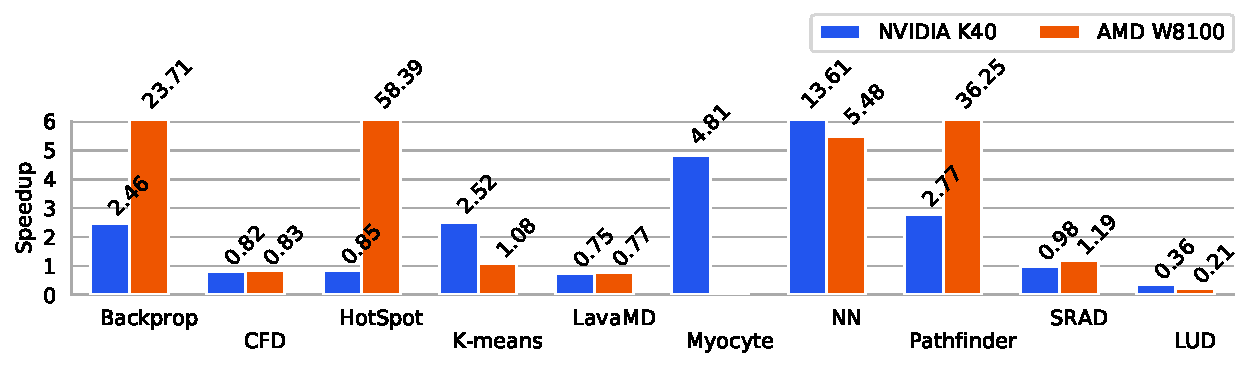
\includegraphics[scale=0.65]{experiments/rodinia.pdf}
  \caption{Relative speedup compared to reference implementations for
    Rodinia (the bar for NN is truncated for space reasons).}
  \label{fig:rodinia-speedup}
\end{figure*}

Rodinia is a popular benchmark suite that contains approximately $21$
benchmarks.  Of these, we have selected those $10$ benchmarks that
look the most friendly from a data-parallel perspective, and were
expressible in terms of a nested composition of \kw{map}, \kw{reduce},
\kw{scan}, \StreamRed{}, \StreamMap{}.

There is great variation in the performance of the Rodinia reference
implementations.  Some, such as Myocyte or NN, contain oversights that
negatively affect GPU performance.  Others, such as LUD or LavaMD, are
based on clever algorithms and carefully implemented.  Some Rodinia
implementations exhibit massive slowdown on the AMD GPU for reasons
that we cannot determine.  We conjecture that this is related to the
under-powered CPU on the machine hosting the AMD GPU, but this is only
a suspicion.  The speedups are shown on \cref{fig:rodinia-speedup}.

The speedup on Backprop seems related to a reduction that Rodinia has
left sequential.  Running time of the training phase is roughly equal
in Rodinia and Futhark ($\sim10~ms$).

Rodinia's implementation of HotSpot, a two-dimensional stencil code,
uses time tiling~\cite{HexaTiling}, which seems to pay off on the
NVIDIA GPU, but not on AMD.  On the NVIDIA GPU, the majority of
Futhark's slowdown is due to how memory management is done for the
arrays involved in the time series loop in the stencil.  At a high
level, the stencil is a sequential loop containing a nested \kw{map}
over the $m\times{}m$ iteration space:

\begin{lstlisting}
loop s = s0 for i < n do
  let s' = map (\i -> map (f s i) [0...m-1]) [0...m-1]
  in s'
\end{lstlisting}

Two distinct memory blocks are necessary, because several elements of
\lstinline{s} are combined to construct one element of \lstinline{s'}.
The reference implementation uses two pre-allocated buffers, and
switches between them by swapping the pointers.  This is a common
technique for implementing stencils.  Instead of swapping pointers,
The Futhark compiler copies the entire intermediate result instead,
and these copies account for $30\%$ of runtime.

Our speedup on $k$-means is due to Rodinia not parallelising
computation of the new cluster centres, which is semantically a
histogram, which can be implemented as a segmented reduction.

The default dataset for Myocyte dataset was expanded because its
degree of parallelism was one ($\texttt{workload}=1$).  We used
Rodinia's CUDA implementation rather than its OpenCL implementation,
as the latter is not fully parallelised.  We attribute our speedup to
automatic coalescing optimisations, which is tedious to do by hand on
such large programs.

Our speedup on NN is due to Rodinia leaving $100$ \kw{reduce}
operations for finding the nearest neighbours sequential on the CPU.
This is possibly because the reduce operator is atypical: it computes
both the minimal value and the corresponding index, much like the
example in \cref{sec:choice-of-parallel-combinators}.  Speedup is less
impressive on the AMD GPU, due to higher kernel launch overhead---this
benchmark is dominated by frequent launches of short kernels.

For Pathfinder, Rodinia uses time tiling, which, unlike HotSpot, does
not seem to pay off on the tested hardware.

The reference implementation of LUD uses a clever block-based
algorithm that makes efficient use of local memory on the GPU.  The
Futhark implementation is similar, but the Futhark compiler is not yet
able to map it as efficiently to the GPU hardware.  The LUD algorithm
uses block decomposition, and the block size (not to be confused with
the CUDA term ``thread block size'', which is something else) is a
programmer-given constant.  Both the reference and Futhark
implementation simply hard-code a constant that appears to give good
performance in practise: $32$ for Futhark, and $16$ for the reference
implementation.

\subsection{Four Benchmarks from Parboil}

\begin{figure*}
  \centering
  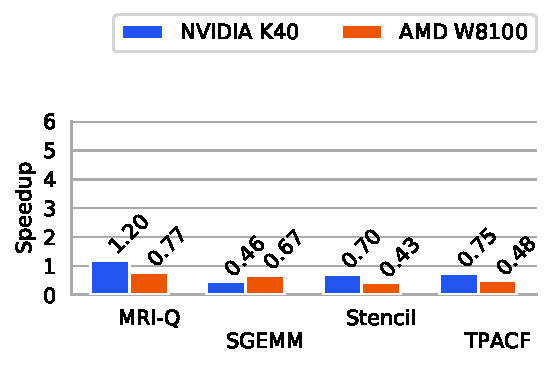
\includegraphics[scale=0.65]{experiments/parboil.pdf}
  \caption{Relative speedup compared to reference implementations for Parboil.}
  \label{fig:parboil-speedup}
\end{figure*}

The Parboil benchmark suite is smaller than Rodinia, containing $11$
benchmarks, but the implementations are generally of higher quality.
Furthermore, Parboil comes with excellent built-in support for
instrumentation and validation of results.  The Parboil benchmarks
tend to be more difficult than those found in Rodinia, so we have only
ported four of them to Futhark.  The speedups are shown on
\cref{fig:parboil-speedup}.

MRI-Q is semantically an outer \kw{map} surrounding an inner
\kw{map}-\kw{reduce} operation on an array that is invariant to the
outer \kw{map}.  The Parboil implementation is based on heavily
unrolling the inner loop, while the Futhark compiler performs
one-dimensional tiling in local memory
(\cref{sec:one-dimensional-tiling}).  This appears to be the superior
strategy on the NVIDIA GPU, but not the AMD GPU.

SGEMM is an implementation of a common matrix primitive that computes
\[
  C \leftarrow \alpha \times A \times B + \beta \times C
\]
where $A,B,C$ are matrices and $\alpha,\beta$ are scalars.  The
Futhark compiler performs two-dimensional tiling
(\cref{sec:two-dimensional-tiling}) in local memory, while the Parboil
implementation performs more sophisticated \textit{register tiling}.
SGEMM is a well-studied primitive, and it is hard for a compiler to
match a hand-tuned implementation.

Stencil is a straightforward stencil code.  The Futhark implementation
suffers due to poor memory management that induces extra copies, as
with Rodinia's HotSpot.

TPACF is semantically a histogram, which Parboil implements using
clever use of local memory.  In Futhark, we implement it using a
segmented reduction, which is not as efficient.

\subsection{Two Benchmarks from FinPar}
\label{sec:finpar}

\begin{figure*}
  \centering
  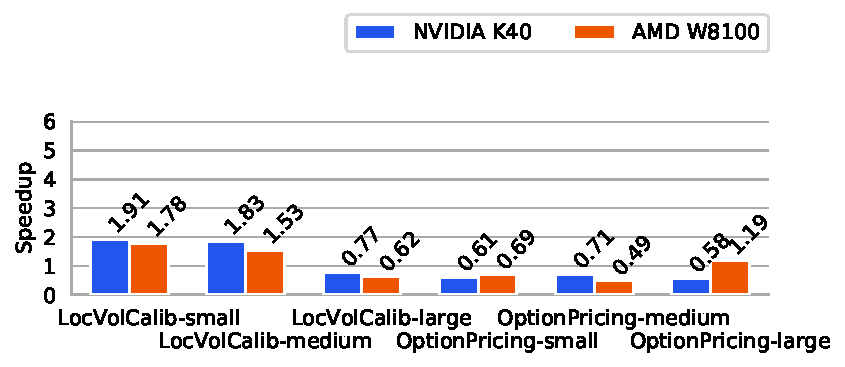
\includegraphics[scale=0.65]{experiments/finpar.pdf}
  \caption{Relative speedup compared to reference implementations for
    FinPar.  Each benchmark is applied to three different data sets.}
  \label{fig:finpar-speedup}
\end{figure*}

FinPar is a small benchmark suite translated from real-world financial
kernels.  The problems are sophisticated, with nontrivial use of
nested parallelism, and the reference implementations are well
implemented.  We have ported only two out of the three FinPar
benchmarks to Futhark, as the third one (InterestCalib) contains
(limited) irregular parallelism.  Due to the small size of FinPar, we
have evaluated each benchmark on all three available data sets.  The
speedups are shown on \cref{fig:finpar-speedup}.

OptionPricing is essentially a \kw{map}-\kw{reduce}-composition.  The
benchmark primarily measures how well the Futhark compiler
sequentialises excess parallelism inside the complex \kw{map}
function.  We see approximately equal relative performance for each of
the three data sets.

LocVolCalib from FinPar is an outer \kw{map} containing a sequential
\kw{for}-loop, which itself contains several more \kw{map}s.
Exploiting all parallelism requires the compiler to interchange the
outer \kw{map} and the sequential loop.  The slowdown on the AMD GPU
is due to transpositions, inserted to fix coalescing, being relatively
slower than on the NVIDIA GPU.

The \textit{small} and \textit{medium} datasets for LocVolCalib have
the interesting property that they do not provide enough parallelism
in the outer loops to fully saturate the GPU.  Note the absolute
runtime numbers on \cref{tab:benchmarks}, where the runtime for the
\textit{small} dataset is greater than that for the \textit{medium}
dataset, despite the latter actually requiring more work.  Two
distinct LocVolCalib implementations are provided by FinPar: one that
exploits only outer-level parallelism, and one that exploits
\textit{all} available parallelism.  The former is the right choice for
the \textit{large} dataset, and the one we compare against here, as it
is also roughly how the current Futhark compiler parallelises
LocVolCalib.  However, the FinPar implementation that fully exploits
all parallelism outperforms Futhark on the small and medium datasets.
Handling cases such as this transparently is the main motivation for
multi-versioned code (\cref{sec:multi-versioned-code}).

\subsection{Five Benchmarks from Accelerate}
\label{sec:accelerate}

\begin{figure*}
  \centering
  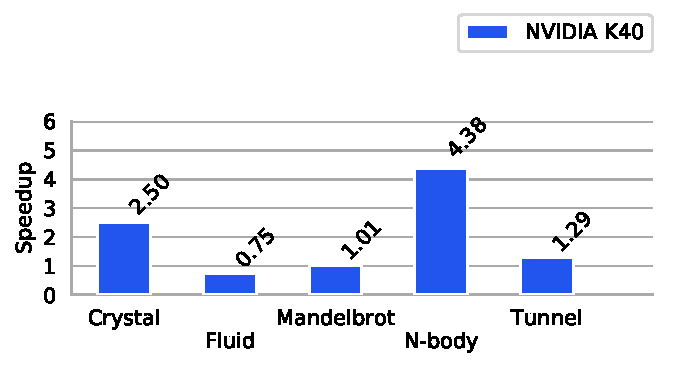
\includegraphics[scale=0.65]{experiments/accelerate.pdf}
  \caption{Relative speedup compared to reference implementations for
    Accelerate.}
  \label{fig:accelerate-speedup}
\end{figure*}

Accelerate is a mature Haskell-embedded language for data-parallel
array programming.  The benchmarks picked here are presented as
``examples'', and are not part of a benchmark suite as such.  While
they are written by the Accelerate authors themselves, and contain
built-in support for benchmarking, it is possible that performance has
been sacrificed in the interest of readability.  We use the recently
released \texttt{llvm-ptx} GPU backend, which performs significantly
better than the old \texttt{cuda} backend.  Unfortunately, this
backend is still NVIDIA-specific, so we were unable to execute
Accelerate on the AMD GPU.

The benchmarks were all straightforward to translate to Futhark, as
Accelerate does not support nested parallelism or low-level GPU
programming.  One major and interesting source of performance
differences is that Accelerate is a Just-In-Time (JIT) compiler for an
embedded language, while Futhark is a conventional Ahead-Of-Time (AOT)
compiler.  As a result, Accelerate has access to dynamic information
that can be used to perform code specialisation, but its embedded
nature limits the compilers ability to see the program as a whole.  On
the other hand, the Futhark compiler can perform more global
optimisations, but cannot inline dataset-specific constants for loop
iteration counts and similar.  The trade-offs between JIT and AOT
compilation are a fascinating and deep subject that we will not delve
further into here, but is certainly worthy of further study.  Speedups
are shown on \cref{fig:accelerate-speedup}.

Crystal is a straightforward \kw{map} containing an inner
\kw{map}-\kw{reduce} over a small array.  It is unclear why
Futhark outperforms Accelerate on this benchmark.

Fluid is a two-dimensional stencil code with complicated edge
conditions.  As with Rodinia's HotSpot, Futhark's approach to memory
management causes unnecessary copies for each of the outer sequential
loops, giving Accelerate the edge.

The Mandelbrot benchmark is a straightforward \kw{map} containing a
\kw{while} loop, with little opportunity for optimisation.

$N$-body is operationally a \kw{map} containing an inner
\kw{map}-\kw{reduce} over an array invariant to the outer array.  The
Futhark compiler performs one-dimensional tiling in local memory to
optimise access to this array.  Accelerate does not perform tiling,
which gives the edge to Futhark.

Tunnel is similar to Crystal, and contains a straightforward \kw{map}
containing an inner \kw{map}-\kw{reduce} over a small array.
Performance is similar between Futhark and Accelerate.

\subsection{Impact of Optimisations}
\label{sec:impact-of-optimisation}

Impact was measured by turning individual optimisations off and
re-running benchmarks on the NVIDIA GPU.  We report only where
the impact is non-negligible.

Fusion (\cref{chap:fusion}) has a significant impact on K-means
($\times1.42$), LavaMD ($\times4.55$), Myocyte ($\times1.66$), SRAD
($\times1.21$), Crystal ($\times10.1$), and LocVolCalib ($\times9.4$).
Without fusion, OptionPricing, N-body, MRI-Q, and SGEMM fail due to
increased storage requirements.

In the absence of in-place updates, we would have to implement K-means
as on Figure~\ref{fig:parallel-means}---the resulting program is
slower by $\times8.3$.  Likewise, LocVolCalib would have to implement
its central \lstinline{tridag} procedure via a less efficient
\lstinline{scan}-\lstinline{map} composition, causing a $\times1.7$
slowdown.  OptionPricing uses an inherently sequential Brownian Bridge
computation that is not expressible without in-place updates.

The coalescing-by-transposition transformation
(\cref{sec:automatic-coalescing}) has a significant impact on
$k$-means ($\times9.26$), Myocyte ($\times4.2$), OptionPricing
($\times 8.79$), and LocVolCalib ($\times 8.4$).
%
Loop tiling (\cref{sec:automatic-tiling}) has an impact on LavaMD
($\times 1.35$), MRI-Q ($\times1.33$), SGEMM ($\times2.3$), $N$-body
($\times 2.29$), and LUD ($\times 1.10$).

\section{Benchmarking an implementation of Breadth-First-Search}
\label{sec:bfs-benchmarking}

The Rodinia benchmark suite contains a benchmark, BFS, that
implements Breadth-First-Search.  This problem is highly irregular,
and its performance is very dataset-sensitive.  As a result, we have
excluded it from the presentation of the general benchmark results,
and instead dedicated this section to discuss the issues.  The
following serves as an example of benchmarks where measuring
performance is not quite straightforward, and incidentally as an
example of how to implement irregular problems in Futhark.

Figure~\ref{fig:bfs-imperative} shows an excerpt of Rodinia's
imperative-but-parallel implementation of the breadth-first search
algorithm, which traverses the graph and records in the
\lstinline{cost} array the breadth level of each graph node.
%
The code excerpt processes in parallel all the nodes, indexed by \lstinline{src_id},
on the current breadth level (i.e., the ones with the \lstinline{mask[src_id]} set).
%
For each such node, the breadth level of all its unvisited neighbours
(i.e., \lstinline{!visited[id]}) are updated to \lstinline{cost[src_id]+1} in the
sequential (inner) loop at line \ref{line:seqcostupd}.
%
The problem with this code is that the update of \lstinline{cost}
potentially introduces data races in the case when two nodes on the
same level are connected to a common (unvisited) node.  What makes it
still safe is the property that the output dependences are idempotent
(i.e., the updated value is the same across different outermost
iterations).

Figure~\ref{fig:bfs-fun-pad} shows a simple, albeit work-inefficient,
translation to Futhark of the discussed imperative code, which uses
padding to satisfy array regularity. First, the indices of the active
nodes (i.e., the ones on the current breadth level) are identified by
the \lstinline{filter} operation on line \ref{line:futfilter}.  This
contributes significantly to final performance.  Second, the maximal
number of edges of these nodes, denoted by \lstinline{e_max}, is
computed via a \lstinline{map-reduce} composition on lines
\ref{line:emaxstart}--\ref{line:emaxend}.  Third, the \lstinline{map}
nest computes two two-dimensional arrays of innermost size equal to
\lstinline{e_max}, in which the first one corresponds to the indices
of the unvisited neighbours, and the second one to their breadth level
(\lstinline{costs}).  The indices that are outside the edge degree of
a node are marked with out-of-bounds indices (\lstinline{-1}), and
similarly for the nodes that were already visited.
%
Fourth, the index-value arrays are flattened (at lines
\ref{line:futflatstart}-\ref{line:futflatend}) and the
\lstinline{scatter} bulk operator is used to update the
\lstinline{cost} and \lstinline{updating_mask} arrays at lines
\ref{line:futupdatestart}--\ref{line:futupdateend}.

Table~\ref{fig:bfs-speedup} shows the running time of Futhark and
Rodinia implementations on four datasets. The Rodinia implementation
exploits only the parallelism of the outer loop, and it wins on the
datasets in which the graph is large enough to fully utilise the
hardware, while Futhark exploits both levels of parallelism and wins
on smaller graphs with large edge degree.  Interestingly, this is not
simply a question of how much to parallelise, but a fundamental
algorithmic design decision.  The unsolved challenge is a
representation and technique that can fuse the Futhark code in
\cref{fig:bfs-fun-pad} into something resulting the one-level-parallel
C code in \cref{fig:bfs-imperative}, and furthermore generate both
versions of the code.

\begin{figure}[ht]
\begin{lstlisting}[xleftmargin=0pt,language=C,numbers=left,escapechar=|]
// n is the number of graph nodes
for (int src_id = 0; src_id < n; src_id++ ) { // parallel
    if (mask[src_id] == true) {
        mask[src_id] = false;
        for (int i = nodes[src_id].starting; // sequential
             i < (nodes[src_id].num_edges
                  +nodes[src_id].starting);
             i++) {
            int dst_id = edges_dest[i];
            if(!visited[dst_id]) {
                cost[dst_id] = cost[src_id] + 1; |\label{line:seqcostupd}|
                updating_mask[dst_id] = true;
            }
        }
   }
}
\end{lstlisting}
  \caption{Imperative code for breadth-first search.}
  \label{fig:bfs-imperative}
\end{figure}

\begin{figure}[ht]
\small
\begin{lstlisting}[xleftmargin=0pt,language=futhark,numbers=left,escapechar=|]
let step [n][e] (cost: [n]i32)
                (nodes_starting: [n]i32)
                (nodes_num_edges: [n]i32)
                (edges_dest: [e]i32)
                (visited: [n]bool)
                (mask: [n]bool)
    : ([n]i32, [n]bool, []i32) =
  let active_indices = filter (\i -> mask[i]) (iota n)|\label{line:futfilter}|
  let n_indices = length active_indices
  let e_max = |\label{line:emaxstart}|
    reduce i32.max 0
    (map (\i -> nodes_n_edges[i]) active_indices)|\label{line:emaxend}|
  let (node_ids_2d, costs_2d) =
    map (\src_id: ([e_max]i32, [e_max]i32)  ->
          let s_index = nodes_starting [src_id]
          let n_edges = nodes_num_edges[src_id]
          let edge_indices = map (+s_index) (iota e_max)
          let node_ids =
            map (\i ->
                  if i < s_index + n_edges
                  then let dst_id = edges_dest[i]
                       in  if !visited[dst_id]
                           then dst_id else -1
                  else -1)
                edge_indices
          let costs = replicate e_max (cost[src_id] + 1)
          in (node_ids, costs))
         active_indices
  let node_ids = reshape flat_len node_ids_2d |\label{line:futflatstart}|
  let costs = reshape flat_len costs_2d |\label{line:futflatend}|
  let flat_len = e_max * n_indices
  let mask' = |\label{line:futupdatestart}|
    scatter mask active_indices (replicate n_indices false)
  let cost' =
    scatter cost node_ids costs
  let updating_mask' =
    scatter updating_mask node_ids (replicate flat_len true) |\label{line:futupdateend}|
  in (mask', cost', updating_mask')
\end{lstlisting}
  \caption{Work-inefficient Futhark code for breadth-first search.}
  \label{fig:bfs-fun-pad}
\end{figure}

Finally, we remark that the presented Futhark code is work-inefficient
due to the ``padding'' of the edge-degree of a node, but the
\lstinline{scatter} construct also enables a work-efficient
implementation (not shown), which would correspond to applying
flattening by hand. In our tests, this is slower than the padded one
due to the overhead of multiple scans.
%

\begin{table*}
  \centering
  \begin{tabular}{llrr}
    \textbf{Dataset} & \textbf{Version} & \textbf{Runtime} & \textbf{Speedup} \\

    \multirow{2}{*}{2000 nodes, 1000 edges each} & Futhark & 4.0ms & \multirow{2}{*}{$\times1.9$} \\\cline{2-3}
                     & Rodinia & 7.6ms \\\hline

    \multirow{2}{*}{1000 nodes, 10--1000 edges each} & Futhark & 1.7ms & \multirow{2}{*}{$\times3.7$} \\\cline{2-3}
                     & Rodinia & 6.3ms \\\hline

    \multirow{2}{*}{100,000 nodes, 6 edges each} & Futhark & 6.7ms & \multirow{2}{*}{$\times0.25$} \\\cline{2-3}
                     & Rodinia & 1.7ms \\\hline

    \multirow{2}{*}{100,000 nodes, 10--500 edges each} & Futhark & 153.1ms & \multirow{2}{*}{$\times0.43$} \\\cline{2-3}
                     & Rodinia & 66.5ms \\\hline

  \end{tabular}
  \caption{Performance of Rodinia and Futhark breadth-first search
    implementations on various datasets. Executed on an NVIDIA GTX 780
    Ti with random graphs (uniform distribution).  Reported runtime is
    average over $10$ runs.}
  \label{fig:bfs-speedup}
\end{table*}

%%% Local Variables:
%%% mode: latex
%%% TeX-master: "thesis"
%%% End:


\chapter{Interoperability}

%%% Local Variables:
%%% mode: latex
%%% TeX-master: "thesis"
%%% End:


\clearpage

\part{Closing Credits}

% We want the bibliography in the ToC, but it shouldn't have a chapter
% number.
\phantomsection
\addcontentsline{toc}{chapter}{Bibliography}
\defbibheading{bibliography}{\chapter*{Bibliography}}
\printbibliography

\backmatter
\appendix
\input{appendix.tex}

\end{document}

%%% Local Variables:
%%% mode: latex
%%% TeX-master: t
%%% End:
